\documentclass[a4paper,12pt, DIV=14, BCOR=5mm, twoside, headsepline]{scrbook}

\usepackage{mathtools}
\usepackage{amsmath}
\usepackage{amsfonts}
\usepackage{amsthm}
\usepackage{verbatim}
\usepackage[cal=boondoxo]{mathalfa}
\usepackage{relsize}
\usepackage[boxruled, linesnumbered]{algorithm2e}
\usepackage{stmaryrd}


\usepackage{hyperref}
\hypersetup{
    colorlinks,
    citecolor=black,
    filecolor=black,
    linkcolor=black,
    urlcolor=black
}

\usepackage{tikz}

\usepackage[utf8]{inputenc}

\setcounter{MaxMatrixCols}{20}

\pagestyle{headings}

\renewcommand*{\dictumwidth}{0.65\textwidth}
\renewcommand*{\raggeddictum}{\centering}
\renewcommand*{\raggeddictumtext}{}
\setkomafont{dictumtext}{\normalfont\normalcolor\itshape\setlength{\parindent}{2em}\noindent}

\newcommand{\bigzero}{\mbox{\normalfont\Large\bfseries 0}}


\newtheorem{theorem}{Theorem}[section]
\newtheorem{corollary}{Corollary}[theorem]
\newtheorem{lemma}[theorem]{Lemma}
\newtheorem{definition}{definition}[section]
\newtheorem*{remark}{Remark}
\newtheorem{example}{Example}[chapter]


\usepackage[backend=biber, style=alphabetic, sorting=ynt]{biblatex}
\addbibresource{references.bib}

\AtEveryBibitem{%
  \ifentrytype{misc}{%
  }{%
    \clearfield{url}%
  }%
}

\usepackage{xkeyval}

%citation nasa ads macros

\def\apjl{\textit{ApJ}}                % Astrophysical Journal, Letters

\def\prd{\textit{Phys.~Rev.~D}}        % Physical Review D

\def\prl{\textit{Phys.~Rev.~Lett.}}    % Physical Review Letters


\title{Covariant Constructive Gravity}
\author{Tobias Reinhart }
\date{April 2019}

\begin{document}

\maketitle

\tableofcontents

\chapter{Introduction: The Aim of Constructive Gravity}

%in introduction: main idea of constructive gravity and reasons for the constructive approach. Maybe also current state of the field (+ lovelock, HKT, bootstrap).



Before we start with the main part we quickly illustrate particularities of the chosen \textit{\textbf{notation}}. Throughout this thesis even if not stated explicitly all objects are considered to be smooth, i.e. we work with smooth maps defined on smooth manifolds. 

Furthermore as the relevant construction presented in this work are entirely local we will denote maps between manifolds without being to rigorous with the description of the appropriate domain and codomain respectively. Hence we might for instance write $x^a : M
\rightarrow \mathbb{R}$ for a chart map on a manifold $M$ where we should more properly write $x^a : M \supset U : \rightarrow x(U) \subset \mathbb{R} $. 

Lower case latin indices $a,b,c,...$ are used as spacetime indices and hence run from 0 to 3, spatial indices between 1 and 3 are denoted by lower case greek letters $\alpha,\beta,\gamma,...$. In addition to that we will use further types of indices to describe coordinate functions on additional bundles that we are going to construct over the spacetime manifold $M$. Upper case latin letters from the middle of the alphabet $I_k,J_k,L_k,...$ will be used to describe derivative indices of order $k$ and hence run from $0$ to $\binom{b+k-1}{n-1}-1$ where $n$ is the dimension of the basespace w.r.t. which the derivatives are taken. As we will work extensively over some second order jet bundle we will sometimes drop the labels that specify the order of such indices and hence use $I,J,K,...$ to solely describe such second derivative order indices if this does not cause confusion.

There will also be situations with two different types if derivative indices appearing in the same equation, describing higher derivatives w.r.t. the coordinates of the spacetime manifold and w.r.t. coordinates of some additional bundle. We will then label the derivative coordinates of the latter kind by caligraphic letters $\mathcal{I}_k, \mathcal{J}_k,...$ to allow for distinction.

Upper case latin letters from the beginning of the alphabet $A,B,C,D,...$ are used to label fibre coordinate functions on the space of fields, whenever we are dealing with a second field that belongs to a different space we label the coordinates by $\tilde{A}, \tilde{B},...$ . The respective range obviously depends on the specific field at hand.\\

In this work we will deal with bundles of smooth manifolds to quite some extend. When we introduce a new bundle we will denote it as triple $(F,\pi_F,M)$ consisting of the total space $F$ the bundle projection $\pi_F$ and the base space $M$. Priorly introduced bundles might also be simply denoted by their total space. Morphisms between bundles $(F_1,\pi_1,M_1)$ and $(F_2,\pi_2,M_2)$ are denoted as pairs of maps $(f,h)$, with $f$ being the map between total spaces that covers $h$. Bundle morphisms that cover the identity or such morphisms that are constructed from a given map between base spaces will be referred simply by the map on the total space.

Given a vector space $V$, a linear map $\phi$, a vector bundle $(E,\pi,N)$ or any other object with a notion of duality, a superscripted $\ast$ on the relevant object will denote the corresponding dual object, i.e. the dual vector space $V^{\ast}$, dual linear map $\phi^{\ast}$, dual vector bundle $(E^{\ast}, \pi^{\ast},N)$. In particular given a smooth map between manifolds $f : M \rightarrow N$ we denote its pushforward by $f_{\ast} : Tm \rightarrow TN$ and its pullback by $f^{\ast} : T^{\ast}N \rightarrow T^{\ast}M$.

We denote tensor products by $\otimes$ and the corresponding space of $(m,n)$ tensors over $M$ by $T^m_nM$. The space of n-forms over $M$ is denoted by $\Lambda^nM$. Given a bundle $(F,\pi_{F},M)$ we write $G \in \Gamma(F) $ for a section of this bundle. We denote direct sums of vectorspaces or the whitney sum of vector bundles by $\oplus$ respectively. \\

The jet bundle of order q over a given bundle $(F,\pi_F,M)$ will be denoted by $J^qF$ and any associated jet prolongation map, either in the sense of prolonging sections of $F$ to sections of $J^qF$ or in the sense of prolonging vectorfields on $M$ to vectorfields on $J^qF$ will be referred to as $j^q$. 

In general we will label bundle maps that take values in the bundle of volume forms over some base manifold letters in calligraphic font $\mathcal{L}, \mathcal{H}$ and the corresponding representation in terms of the chart induced volume form by the corresponding standard font letter $\mathcal{L}=L \mathrm{d}^4x, \mathcal{H}= H \mathrm{d}^3x$.

As usual $\left[ \  ,   \  \right]$ denotes the commutator of vector fields and $\left \{  \  ,   \   \right \}$ the poisson bracket of phase space functions/functionals. 

\chapter{Diffeomorphism invariant field theory}

\dictum{
We provide the basic mathematical tools necessary for a precise formulation of classical Lagrangian field theory. Furthermore we study implications of the requirement that the Lagrangian be infinitesimally equivariant w.r.t. spacetime diffeomorphisms and derive from it an equivalent set of first order partial differential equations. Lastly we investigate consequences of the diffeomorphism invariance for the Hamiltonian formulation of classical field theory.
}

\section{Field bundles jet bundles and prolongations}
In order to develop a concise framework for classical Lagrangian field theory it is insightful to recall the situation in standard classical mechanics. There one encodes the possible configurations a given system might adopt at given time as finite dimensional manifold, the so called configuration space $Q$. The objects of interest are curves $\gamma : \mathbb{R} \rightarrow Q $ that represent the systems path in this configuration space, i.e. the particular system configuration dependent on some parameter time. Given such a curve, by adjoining its velocity $\dot{\gamma}$ at each parameter value one can lift the curve to the tangent bundle $TQ$. The dynamics of the system can then be described by a Lagrangian function $L : TQ \rightarrow \mathbb{R}$. Composing $L$ with a lifted curve one obtains a real valued function. As such one can compute its integral. This procedure defines a local functional on the space of curves:
\begin{align}
S[\gamma] = \int \mathrm{d}\lambda L(\gamma (\lambda), \dot{\gamma} (\lambda)).  
\end{align}
Fixing start and end configuration and velocity of the system for all curves in consideration, the physical curves are those that extremize this action functional, or equivalently those that solve the corresponding Euler-Lagrange-Equations. \\

%We conclude that in order to obtain a mathematical precise formulation of classical mechanics one needs a manifold that represents possible system configurations, %a notion of lifting curves in this configuration space by adjoining its velocities and a Lagrangian function that encodes the dynamics of the system.\\

Once the transition from standard particle mechanics to field theories is made the system is no longer described by curves in some finite dimensional configuration space representing the systems configuration at each parameter time, but by the values a given field attains at different spacetime points. Hence instead of curves one deals with sections of some bundle $(F,\pi_F,M)$ over the 4-dimensional spacetime manifold $M$. The notion of adjoining velocities to a curve is replaced by adjoining derivatives to a section. The appropriate setting for this procedure is the \textit{\textbf{jet bundle}} over $F$. Just as the tangent bundle $TQ$ is obtained from a coordinate independent description of derivatives of curves, the jet bundle over $F$ is constructed by a coordinate independent description of derivatives of sections of $F$. As before the Lagrangian is then simply a function on this jet bundle. 
In the following we outline how these ideas can be cast into precise mathematical language. \\

We follow \cite{1998physics...1019G} to some extend. Further information concerning the geometry of jet bundles can be found in \cite{saunders_1989} and \cite{seiler2009involution}. Many details regarding the involved standard differential geometry are collected in \cite{doi:10.1142/3867}. Let $M$ be an oriented 4-dimensional manifold that represents spacetime. We restrict our attention to tensor fields over $M$. Such fields are \textit{\textbf{sections}} of a bundle $(F,\pi_F,M)$, i.e. smooth maps $G : M \rightarrow F $ that satisfy $\pi_F \circ G = \mathrm{id}_M$. In the following we will refer to the bundle $F$ as $\textit{\textbf{field bundle}}$.  As we want to consider tensor fields the field bundle is required to be given by a vector sub bundle of some $T^m_n M$. We denote adapted coordinates\footnote{Recall that adapted coordinates $(x^m,v_A)$ on a fibre bundle $(F, \pi_F, M)$ are defined by the requirement that there exits a coordinate chart on $M$, $(y^m)$, s.t. $y^m = x^m \circ \pi_F$, and hence we denote the first $dim(M)$ coordinate functions of both charts with the same label. It should be clear from the context which coordinates are meant, those on $M$ or those on $F$.} on $F$ by $(x^m,v_A)$, where $A$ runs from $0$ to $n - 1$ with $n$ being the fibre dimension of $F$, i.e. $n := \pi_F^{-1}(p)$ for some $p \in M$. Note that as $F$ is assumed to be a vector bundle we can always chose adapted coordinates s.t. the $v_A$ are linear on the fibres. Details regarding this remark can be found in \cite{saunders_1989}. In the following we will only regard such adapted coordinates. The corresponding coordinate representation of sections is denoted by $G_A(x^m(p)) = v_A \circ G (p)$ where we will simply write $G_A$ most of the time. Hence writing $G_A$ we refer to the coordinate representation of a section, whereas $v_A$ simply denotes fibre coordinates on $F$. \\
%check coordinate expression 

Given a field bundle $(F, \pi_F, M)$ we can define the corresponding $\textit{\textbf{dual field bundle}}$ $(F^{\ast}, \pi_{F^{\ast}},M)$ as its vector bundle dual. We quickly recall the definition of the vector bundle dual and the dual of a linear map.
\begin{definition}[dual linear map] \label{dual}
Given vectorspaces $V$ and $W$ and a linear map, i.e. a morphism of vectorspaces $f : V \rightarrow W$, the dual linear map $f^{\ast} : W^{\ast} \rightarrow V^{\ast}$ is defined by the requirement: 
\begin{align}
    \forall v \in V, \forall \omega \in W^{\ast} : \omega (f(v)) = f^{\ast}(\omega) (v).
\end{align}
\end{definition}
Sometimes the dual of a linear map is also called its adjoint. With the definition of the vector space dual and the dual of a linear map we can now lift these notions to the case of vector bundles and vector bundle morphisms.
\begin{definition} [vector bundle dual]
Given a vector bundle $(F, \pi_F,M)$. Its vector bundle dual is the vector bundle $(F^{\ast}, \pi_{F^{\ast}},M)$ with fibres $\pi_{F^{\ast}}^{-1}(p) = (\pi_F^{-1}(p))^{\ast} $ for all $p$ in $M$ and the obvious projection.  
\end{definition}
In other words one obtains the dual to a given vector bundle by implementing the dual construction fibre by fibre.
Given adapted coordinates on the field bundle $(x^m, v_A)$ with the coordinate functions $v_A$ being linear on the fibres, we can obtain \textbf{\textit{dual coordinates}} on the dual field bundle by $(x^m, ((v_A)^{\ast})^{-1})$, i.e. by taking the inverse dual of the fibre coordinates $v_A$ (see \cite{saunders_1989}). Note that we do not simply take the dual of the $v_A$ but its inverse as the dual construction reverses the direction of linear maps\footnote{In the language of category theory: duality defines a contravariant functor.}. In the following we denote the fibre coordinates dual to $v_A$ by $v^A$. With these coordinates we get $ v_A(v^B) = \delta_A^B$. From now on given a chart on the field bundle we always work with the corresponding dual chart on the dual field bundle.\\
%check this last statement

Note that as the field bundle is required to be given by a vector sub bundle of some $T^m_n M$ one usually works directly on $T^m_n M$ and uses chart induced basis fields $\mathrm{d}x^{a_1}\otimes ... \otimes \mathrm{d}x^{a_m} \otimes \frac{\partial}{\partial x^{b_1}} \otimes ... \otimes \frac{\partial}{\partial x^{b_n}}$ to complete a chart on $M$ to one on $T ^m _ n M$. In the following we denote such coordinates on $T^m_n M$ as $(x^m, v^{a_1 ... a_m}_{b_1 ... b_n})$. The coordinate representation of sections is then given as $G^{a_1 ... a_m}_{b_1 ... b_n}$. Although this is the standard way of representing tensor fields in coordinates it has two significant disadvantages. Firstly the notation gets increasingly complicated once products and contractions of higher ranked fields are involved. Secondly if the field bundle is a true sub bundle of $T^m_nM$ and hence has fibres with dimension less than $4^{(m+n)}$ the chart induced fields simply are to many functions to provide a valid chart on this sub bundle. This is for instance the case considering the field bundle for a metric tensor. The total space of this particular bundle is the space of symmetric rank $(0,2)$ tensors $S^2(T^{\ast}M)$. The typical fibre of the field bundle has dimension $10$. Nevertheless one usually uses the $16$ chart induced basis fields $ \frac{\partial}{\partial x^a}  \otimes \frac{\partial}{\partial x^b}$ to obtain coordinate expressions $g_{ab} = g(\frac{\partial}{\partial x^a},\frac{\partial}{\partial x^b})$ for a section of this field bundle. These component functions then necessarily satisfy $g_{ab} = g_{ba}$ which reduces the fibre dimension from $16$ to $10$. \\

As we are going to deal with the bundle $(F, \pi_F, M)$ in a rather abstract setting we do not follow this practise but stick to true coordinates $(x^m,v_A)$ on $F$. 
In order to relate the thus obtained intrinsic description of $F$ to the one that is provided by considering $F$ as being an embedded sub bundle in $T^m_n M$ we construct vector bundle isomorphisms that allow us to identify the two perspectives. We quickly recall the definition of a \textit{\textbf{(vector-)bundle morphism}}:
\begin{definition}[bundle morphism]
Given two bundles $(F_1, \pi_{F_1}, M)$ and $(F_2, \pi_{F_2}, N)$, a bundle morphism covering $h : M \rightarrow N$ is a smooth map $f : F_1 \rightarrow F_2$ such that the following diagram commutes.
\begin{center}
\begin{tikzpicture}
\node (M) at (0,0) {$M$};
\node (N) at (4,0) {$N$};
\node (F1) at (0,3) {$F_1$};
\node (F2) at (4,3) {$F_2$};
\draw [->] (M) -- node[pos=0.5, below] {$h$} (N);
\draw [->] (F1) -- node[pos=0.5, above] {$f$} (F2);
\draw [->] (F1) -- node[pos=0.5, left] {$\pi_{F_1}$} (M);
\draw [->] (F2) -- node[pos=0.5, right] {$\pi_{F_2}$} (N);
\end{tikzpicture}
\end{center}
\end{definition}
\begin{comment}
\begin{remark}
We normally denote a bundle morphism $f$ that covers $h$ as pair $(f,h)$. For the special case $M=N$ and $h=\mathrm{id}_M$ we shorten the notation to simply $f$. Also we might refer to a bundle morphism by the total space function $f$ if $f$ and $h$ are related via some specified construction, i.e. if $f$ can be obtained uniquely once $h$ is given. 
\end{remark}
\end{comment}
We often consider the case where the bundles carry additional structure on their fibres, for instance in the case of $(F, \pi_F, M)$ being a vector bundle an additional vector space structure. Then one is in particularly interested in those bundle morphisms that preserve the given structure. As an example we define a vector bundle morphism between vector bundles $(F_1, \pi_{F_1}, M)$ and $(F_2, \pi_{F_2}, N)$ as a bundle morphism $(f,h)$ that restricts to a linear map on the fibres of $F_1$, i.e. $\forall p \in M$ the restriction $f \vert_{\pi_{F_1}^{-1}(p)}$ defines a linear map.
With these definitions at hand we can now specify the maps that allow for the transition between the description of the field bundle $F$ as abstract, independent vector bundle and the one obtained from considering it as being embedded in some tensor bundle over $M$.
%Clarification needed
\begin{definition}[Intertwiner]
Let $(F,\pi_F,M)$ be a vector bundle. We call a pair of vector bundle morphisms $(I,J)$ that cover $id_M$,
$I: F \rightarrow T^m_n M$ and $J: T^m_n M \rightarrow F $ that satisfy  $J \circ I = \mathrm{id}_F$ a pair of \textbf{\textit{intertwiners}} for the bundle $(F, \pi_F, M)$.
\end{definition}
Tthe last requirement, namely the existence of a leftinverse to $I$ ensures that $\tilde{I} : F \rightarrow I(F) \subset T^m_nM$ defines a vector bundle isomorphism, and thereby allows us to relate the two distinct points of view.
\begin{comment}
\begin{remark}
Note that the situation is similar to the soldering of a vector bundle to a manifold, where the necessary data is a vector bundle isomorphism between the vector bundle and the tangent bundle of the manifold. The soldering then allows one to identify the vector bundle with the tangent bundle of the manifold. By requiring the existence of $J$, a left inverse of $I$ in the definition presented here, we ensure that $I$ is injective and hence defines an isomorphism if $T^m_n M$ is restricted to the image of $I$. The image of $I$ is obviously a vector sub bundle of $T^m_n M$. In total given the two maps $I$ and $J$ we can identify the field bundle $F$, not considered as being embedded in $T^m_n M$ but as abstract bundle  and with independent coordinate charts $(x^m, v_A)$, with a sub bundle of $T^m_n M$, where we can choose the usual chart induced coordinates $(x^m,v^{a_1 ... a_m}_{b_1 ... b_n})$.
\end{remark}
\end{comment}
%rewrite the above !!!!!
%
%
%
%
%
As the two intertwiner maps are linear maps, they can be understood as $I \in F^{\ast} \otimes T^m_n M$ and $J \in (T^m_nM)^{\ast} \otimes F \cong T^n_m M \otimes F$, where $F^{\ast}$ denotes the total space of the vector bundle dual. 
Once we specify intertwiners $(I,J)$ for the field bundle $F$ we immediately obtain intertwiners for the dual field bundle by means of the standard dual construction. We first take the dual of the intertwiner $I$, $I^{\ast}$. As taking the dual reverse the direction one usually proceeds by inverting $I^{\ast}$. Here this can not be done as $I$ is not invertible but only admits a left inverse. Hence its dual is not invertible. It is however well known that the existence of a left inverse for $I$ implies the existence of a right inverse for $I^{\ast}$. 
%
%add citation here ??
%
In the following we denote this map simply by $(I^{\ast})^{-1}$ but keep in mind that it only provides a right inverse of $I^{\ast}$. Vice versa the existence of a right inverse of $J$ guarantees the existence of a left inverse $(J^{\ast})^{-1}$ of its dual. From the definition of the dual map we further find that $(J^{\ast})^{-1} \circ (I^{\ast})^{-1} = id_{F^{\ast}}$. In total given a pair of intertwiners for the field bundle $(I,J)$ we can obtain a pair of intertwiners for the dual fiedl bundle via this construction, i.e. by $((I^{\ast})^{-1}, (J^{\ast})^{-1})$. \\

We can now choose adapted coordinates $(x^m,v_A)$ on the field bundle and the corresponding dual coordinates $(x^m, v^A)$ on the dual field bundle and chart induced coordinates\footnote{We denote coordinate induced tangent vectors by $\frac{\partial}{\partial x^m}$, the coordinate representation of the action of tangent vectors on functions is denoted as $\partial_m f$. } $(x^m, v^{a_1 ... a_m}_{b_1 ... b_n})$ on $T^m_n M$ and the dual coordinates $(x^m, v^{b_1 ... b_n}_{a_1 ... a_m})$ on its dual $T^n_mM$. Using these charts the maps $I$ and $J$ are represented as follows:
\begin{align} \label{interAbs}
    \begin{aligned}
    &I = I^{A a_1 ... a_m}_{b_1 ... b_n} \cdot v_A \otimes  v^{b_1 ... b_n}_{a_1 ... a_m}\\
    &J = J^{b_1 ... b_n}_{A a_1 ... a_m} \cdot v^A \otimes  v^{a_1 ... a_m}_{b_1 ... b_n}.
    \end{aligned}
\end{align}
Computing similar coordinate expressions for the pair of intertwiners of the dual field bundle $((I^{\ast})^{-1}, (J^{\ast})^{-1})$ one finds that:
\begin{align} \label{dualInterAbs}
    \begin{aligned}
         &(I^{\ast})^{-1} = J^{b_1 ... b_n}_{A a_1 ... a_m} \cdot v^A \otimes  v^{a_1 ... a_m}_{b_1 ... b_n}.\\
         &(J^{\ast})^{-1} = I^{A a_1 ... a_m}_{b_1 ... b_n} \cdot v_A \otimes  v^{b_1 ... b_n}_{a_1 ... a_m}.
    \end{aligned}
\end{align} 
Hence although the constructed intertwiners for the dual field bundle define different maps, their components w.r.t. a given chart are already given by the intertwiners of the field bundle $(I,J)$ if one agrees on chosing the appropriate dual coordinates with a given choice of coordinates. Therefore in the following we will drop the distinction of intertwiners for the field bundle and its dual.  This should not cause confusion, as when working with dual coordinates on the dual field bundle already the index position of the fibre coordinates $v_A$ and $v^{A}$ respectively contains the information regarding which intertwiner relates the these coordinates to those one $T^m_n M$ and $T^n_mM$ respectively. In total we find the following relations connecting the two ways of coordinatising the field bundle and its dual:  
\begin{align} \label{interRel}
    \begin{aligned}
    v^{a_1 ... a_m}_{b_1 ... b_n} = I^{A a_1 ... a_m}_{b_1 ... b_n} \cdot v_{A} \ \ &, \ \  
    v_A = J^{b_1 ... b_n}_{A a_1 ... a_m} \cdot v^{a_1 ... a_m}_{b_1 ... b_n}, \\
    v^{b_1 ... b_n}_{a_1 ... a_m} = J^{b_1 ... b_n}_{A a_1 ... a_m} \cdot v^A \ \ &, \ \ 
    v^A = I^{A a_1 ... a_m}_{b_1 ... b_n} \cdot v^{b_1 ... b_n}_{a_1 ... a_m}, \\
    I^{A a_1 ... a_m}_{b_1 ... b_n} &\cdot J^{b_1 ... b_n}_{B a_1 ... a_m} = \delta^A _ B.
    \end{aligned}
\end{align}
In particular we find that intertwiners defined in this way keep contractions between elements of $F$ and $F^{\ast}$ and all possible higher tensor products that can be obtained from these invariant. In other words, it is equivalent if we compute expressions using the chart induced coordinates or, by means of the intertwiners $(I,J)$, using $(x^m, v_A)$ and the corresponding dual coordinates. \\

In practise one can specify the coordinate expressions $I^{A a_1 ... a_m}_{b_1 ... b_n}$ and $J^{b_1 ... b_n}_{A a_1 ... a_m}$ in order to define coordinates $v_A$ in terms of the chart induced coordinates $v^{a_1 ... a_m}_{b_1 ... b_n}$, i.e. one constructs a valid pair of intertwiners with the desired properties and then defines the fibre coordinates on $F$ by
\begin{align}
    \begin{aligned}
    v_A := J^{b_1 ... b_n}_{A a_1 ... a_m} \cdot v^{a_1 ... a_m}_{b_1 ... b_n}\\
    v^A := I^{A a_1 ... a_m}_{b_1 ... b_n} \cdot  v^{b_1 ... b_n}_{a_1 ... a_m} .
    \end{aligned}
\end{align}
This approach can for instance be used if the field bundle is defined in terms of symmetries the tensor field has to satisfy. These symmetries can be expressed as equalities for the coordinates $v^{a_1 ... a_m}_{b_1 ... b_n}$. For instance considering a total symmetric tensor of rank $(0,3)$ the corresponding equations would read $v_{abc} = v_{acb} = v_{cab} = v_{cba} = v_{bac} = v_{bca}$. Equality under the present symmetries defines an equivalence relation on the set of the $4^{m+n}$ coordinate functions on $T^m_n M$. One then sorts the set of equivalence classes according to some ordering. With each coordinate function $v^{a_1 ... a_m}_{b_1 ... b_n}$ we further associate its multiplicity $\sigma(v^{a_1 ... a_m}_{b_1 ... b_n})$ as the number of elements in its equivalence class. Regarding the previous example we would get: $\sigma(v_{111})=1, \sigma(v_{112})=3, \sigma(v_{123})=6$ and so on. 

Note that this works exactly the same for for antisymmetries, blocksymmetries or any other symmetry at hand.  Now one can define
\begin{align}\label{defI}
    I^{A a_1 ... a_m}_{b_1 ... b_n} \begin{cases} = 1 \ \ \text{if $v^{a_1 ... a_m}_{b_1 ... b_n}$ is an element of the $A^{\text{th}}$ equivalence class counting from 0} \\
                       = 0 \ \  \text{otherwise}.
                            \end{cases}
\end{align}
%By doing so one ends up with coordinates functions on the field bundle such that $v_A$ is identified with the chart induced function $v^{a_1 ... a_m}_{b_1 ... b_n}$ that was chosen as representative of the $A^{\text{th}}$ equivalence class .
$J^{b_1 ... b_n}_{A a_1 ... a_m}$ is then defined such that the pair of intertwiners satisfies the last condition in (\ref{interRel}), i.e. $J$ is chosen as left inverse of $I$. 
\begin{align}\label{defJ}
    J^{b_1 ... b_n}_{A a_1 ... a_m} \begin{cases} = \frac{1}{\sigma(v^{a_1 ... a_m}_{b_1 ... b_n})} \ \  \text{if $v^{a_1 ... a_m}_{b_1 ... b_n}$ is an element of the $A^{\text{th}}$ equivalence class counting from 0}\\
    =0  \ \ \text{otherwise}.
    \end{cases}
\end{align}
Considering again the metric tensor as an example, we have $v_{ab} = v_{ba}$ as only symmetry of the $16$ coordinate functions on $T^0_2M$. We sort the equivalence classes as 
\begin{align}
    \left[[v_{00}], [v_{01}], [v_{02}], [v_{03}], [v_{11}], [v_{12}], [v_{13}], [v_{22}], [v_{23}], [v_{33}]\right ].
\end{align}
Now we define the intertwiner $I$ in terms of the components of the following matrix: 
\begin{equation}\label{interIMet}
I^A_{ab} = \begin{bmatrix}
                1 & & & & & & & & & \\
                & 1 & & & & & & & & \\
                & & 1 & & & & & & & \\
                & & & 1 & & & & & & \\
                & 1 & & & & & & & & \\
                & & & & 1 & & & & & \\
                & & & & & 1 & & & & \\
                & & & & & & 1 & & & \\
                & & 1 & & & & & & & \\
                & & & & & 1 & & & & \\
                & & & & & & & 1 & & \\
                & & & & & & & & 1 & \\
                & & & 1 & & & & & & \\
                & & & & & & 1 & & & \\
                & & & & & & & & 1 & \\
                & & & & & & & & & 1 
            \end{bmatrix}.
\end{equation}
Here the rows run over $(a,b)={(0,0),(0,1),(0,2),...,(3,3)}$ and the columns run from $0$ to $9$. Only non vanishing components are displayed. The inverse intertwiner is then given as: 
\begin{equation}\label{interJMet}
J^{ab}_{A} = \begin{bmatrix} 
                1 & & & & & & & & & & & & & & & \\
                & \frac{1}{2} & & & \frac{1}{2} & & & & & & & & & & &  \\
                & & \frac{1}{2} & & & & & & \frac{1}{2} & & & & & & &  \\
                & & & \frac{1}{2} & & & & & & & & & \frac{1}{2} & & &  \\
                & & & & & 1 & & & & & & & & & &  \\
                & & & & & & \frac{1}{2} & & & \frac{1}{2} & & & & & &  \\
                & & & & & & & \frac{1}{2} & & & & & & \frac{1}{2} & &  \\
                & & & & & & & & & & 1 & & & & &  \\
                & & & & & & & & & & & \frac{1}{2} & & & \frac{1}{2} &  \\
                & & & & & & & & & & & & & & & 1  
            \end{bmatrix},
\end{equation}
now with columns running over $(ab)={(0,0),(0,1),(0,2),...,(3,3)}$ and rows running from $0$ to $9$. By this definition we now have for the metric tensor field $v_1 \cong v_{01}, v_2 \cong v_{0,2},...$.
\begin{remark}
It might be tempting to define the pair of intertwiners in a way such that the matrix representation of $I$ equals the matrix transpose of the matrix representing $J$. This can be achieved by not defining $I$ without fractions and introducing the factors that result from the multiplicities $\sigma$ in $J$, but by splitting them evenly and introducing factors of $\frac{1}{\sqrt{\sigma}}$ both in the definition of $I$ and $J$. Although this seems advantageous there is one particular problem with this definition. The usage of squareroot factors might introduce irrational numbers into the intertwiners. As we are going to rely heavily on computer algebra later and the appearance of irrational numbers severely obstructs the computational performance we stick to the squareroot free approach.  
\end{remark}
%
%reference to problem of constructive gravity in introduction
In the end we want to describe the gravitational field as sections of such a field bundle and construct for it a Lagrangian and the corresponding equations of motion. For that reason it is necessary to introduce a notion of \textit{\textbf{deriving}} such sections. 

It is important to keep in mind that one of the aims of the constructive gravity approach is allowing for a deviation from metric gravity theories. Hence we are not dealing with spacetimes where the usual metric structures are present. In particular there is a priori no distinguished connection on the frame bundle and therefore no covariant derivative that can be used to define derivatives of tensor fields in a coordinate independent fashion. Note however that already in standard general relativity those notions are strictly speaking not necessary. Although there, the fundamental object, the Riemann tensor might be interpreted as curvature 2-form associated to the metric compatible connection on the frame bundle, in coordinates it can be fully written down in terms of the metric tensor its inverse and up to second partial derivatives of the metric without ever mentioning any deeper structure that these expressions might define. The same holds true for the Einstein-Hilbert-Lagrangian. 

We therefore proceed as follows: We keep the involved structures at a minimum, aiming to construct a Lagrangian solely in terms of the gravitational field and partial derivatives of the gravitational field up to some finite order, just as it is the case for the Einstein-Hilbert-Action\footnote{In other words we are not trying to construct structural analogies to general relativity or some other known theory of gravity.}. In order to nevertheless be able to describe partial derivatives of the gravitational field in a well defined, i.e. coordinate independent fashion we construct the $\textit{\textbf{jet bundle}}$ over the field bundle.  \\

The jet bundle over a given bundle can be intrinsically defined in quite abstract fashion. Such an approach nicely reveals its intrinsic properties. This is however not the route we are going to take her as a coordinate based approach to jet bundles is intuitively often more accessible. Furthermore such an approach emphasizes similarities to the construction of the tangent bundle of a manifold. Details regarding the more abstract access to jet bundles can be found in particular in the first chapters of \cite{seiler2009involution}. 
%remark on mathematical precision in the introduction, neglect global properties, etc.
We start by defining the \textbf{\textit{1-jet}} of a \textbf{\textit{section}}.
\begin{definition}[1-jet] 
Given a bundle $(F, \pi_F, M)$, with adapted coordinates $(x^m, v_A)$ and sections $G,H \in \Gamma(F)$, we call $G$ and $H$ 1-equivalent at $p \in M$, if $G(p) = H(p)$ and $\partial_i G_A \vert_p = \partial_i H_A \vert_p$. The corresponding equivalence class of a section $G$ at $p$ is then called the 1-jet of $G$ at $p$ and denoted by $j^1_pG$.
\end{definition}
Here $G_A$ and $H_A$ denote as before the chart representations of the two sections w.r.t. the specified adapted coordinates. One can easily check that this indeed defines an equivalence relations and is independent of the chosen coordinate chart, i.e. well defined. Details can be found in \cite{saunders_1989}. From this definition one immediately sees the similarity to the construction of tangent vectors as equivalence classes of curves. Just as in the case of tangent vectors, where one collects all tangent vectors to obtain the tangent bundle, we can now collect all such 1-jets of sections of $F$ to obtain the first order jet bundle $J^1F$ over $F$. 
\begin{definition}[first jet bundle]
Let $(F, \pi_F, M)$ be a bundle, the first jet bundle over $F$, $(J^1F,\pi_1,M)$ is the bundle with total space $J^1F := \{j^1_pG \ \vert \  p \in M, G \in \Gamma(F)\}$ and bundle projection 
\begin{align*}
    \begin{aligned}
\pi_1 : &J^1F \longrightarrow M \\
&j^1_pG \longmapsto p.
    \end{aligned}
\end{align*}
\end{definition}
\begin{remark}
Note that by this definition $J^1F$ is a bundle over the base manifold $M$. We can also equip $J^1F$ with the projection 
\begin{align}
    \begin{aligned}
    \pi_{1,0} : &J^1F \longrightarrow F \\
    &j^1_pG \longmapsto G(p)
    \end{aligned}
\end{align}
By doing so we additionally provide $J^1F$ with the structure of a bundle over $F$, namely $(J^1F,\pi_{1,0},F)$. From the definition of the two projection we furthermore find that $\pi_1 = \pi_F \circ \pi_{1,0}$. 
\end{remark}
Given adapted coordinates $(x^m,v_A)$ on $F$ we get induced adapted coordinates $(x^m, v_A, v_{Ai})$ on $J^1F$ by defining as always $x^m(j^1_pG) := x^m(p)$, $v_A(j^1_pG) := v_A(G(p))$ and now specifying the new $4 \cdot n$ coordinate functions $v_{Ai}$ by $v_{Ai}(j^1_pG) := \partial_iG_A \vert_p$.
We could now define \textit{\textbf{higher order jet bundles}} in similar fashion, by calling two sections of $F$ \textit{\textbf{q-equivalent}} or equivalent in order $q$ at $p \in M$ if in any coordinate system covering $p$ they agree in their first $q$ partial derivatives evaluated at $p$. There are however arguments why we do not have to work with jet bundles higher than second order if we wish to define a physically meaningful Lagrangian field theory.

As we want to use the jet-bundle formalism to define a Lagrangian and then obtain equations of motion (in short EOM) for the gravitational field as the corresponding Euler-Lagrange Equations the order of the jet bundle is ultimately connected to the order of the highest derivative appearing in the EOM. In the following we want to restrict to cases where the EOM are of no higher than second derivative order. The reason for this restriction is the famous \textbf{\textit{Ostrogratsky}} construction \cite{Ostrogradsky:1850fid}. 
% review this statement 

Simply stated starting from Lagrangians that generate equations of motion with higher than second order time derivatives one obtains instabilities in the associated Hamiltonian formulation. From the perspective of covariant Lagrangian field theory there is no distinct time direction and hence the only way of preventing the theory from these kind of instabilities once we pass to the Hamiltonian formulation is by restricting the Lagrangian such that the generated EOM are of second derivative order altogether. For further information see \cite{2015arXiv150602210W}. 

The appropriate setting for such Lagrangians is the \textbf{\textit{second order jet bundle}}. Although completely analog to the definitions involved in the construction of the first order jet bundle we quickly define the necessary ingredients. 
\begin{definition}[2-jet]
Given a bundle $(F, \pi_F, M)$ with adapted coordinate chart $(x^m, v_A)$ and sections $G,H \in \Gamma(F)$, we call $G$ and $H$ 2-equivalent at $p \in M$, if $G(p) = H(p)$, $\partial_i G_A \vert_p = \partial_i H_A \vert_p$ and $\partial_i \partial_j G_A \vert_ p = \partial_i \partial_j H_A \vert_ p $. The corresponding equivalence class of a section $G$ at $p$ is then called the 2-jet of $G$ at $p$ and denoted by $j^2_pG$.
\end{definition}
Again one can show that this is well defined \cite{saunders_1989}. We collect all such 2-jets for all sections of $F$ and all points in $M$ to obtain the second order jet bundle over $F$.
\begin{definition}[second jet bundle]
Let $(F, \pi_F, M)$ be a bundle, the second jet bundle $(J^2F,\pi_2,M)$ is the bundle with total space $J^2F := \{j^2_pG \  \vert \  p \in M, G \in \Gamma(F)\}$ and bundle projection 
\begin{align*}
    \begin{aligned}
\pi_2 : J^2F \longrightarrow M \\
j^2_pG \longmapsto p.
    \end{aligned}
\end{align*}
\end{definition}
\begin{remark}
One can again show that this really defines a bundle over the base manifold $M$. In the case of the second order jet bundle we can obtain two further bundle projections 
\begin{align*}
    \begin{aligned}
    \pi_{2,1} : &J^2F \longrightarrow J^1F \\
    &j^2_pG \longmapsto j^1_pG ,\\
    \pi_{2,0} : &J^2F \longrightarrow F \\
    &j^2_pG \longmapsto G(p).
    \end{aligned}
\end{align*}
These bundle projections provide $J^2F$ with the additional structure of a bundle over $J^1F$ with projection $\pi_{2,1}$ or a bundle over $F$ with projection $\pi_{2,0}$. Note that from the various definitions we find $\pi_{2} = \pi_F \circ \pi_{2,0} = \pi_F \circ \pi_{1,0} \circ \pi_{2,1}$.
\end{remark}
As before we can obtain adapted coordinates $(x^m, v_A, v_{Ai},v_{Aij})$ of $J^2F$ from adapted coordinates $(x^m,v_A)$ on $F$ by defining $x^m(j^2_pG) := x^m(p)$, $v_A(j^2_pG):= v_A(G(p))$, $v_{Ai}(j^2_pG) := v_{Ai}(j^1_pG)$ and $v_{Aij}(j^2_pG) := \partial_i \partial_j G_A \vert _p$. 
At this point however we run into similar troubles as before, when we tried to use coordinate induced basis vectors to construct a chart on $F$. 

We have specified $4^2\cdot n$ new coordinate functions $v_{Aij}$ to construct adapted coordinates on $J^2F$. Due to the commutativity of the partial derivatives that are involved in the definition the $v_{Aij}$ actually only constitute $4\cdot (4+1)/2 \cdot n = 10\cdot n$ independent functions. To cope with such problems the standard approach is the introduction of multiindices for higher order jet bundles. We will follow a slightly different approach by making use of the same intertwiner technique that we developed before. By doing so it is easier for us to relate the derivative coordinates $v_{Aij}$ and possible higher jet coordinates with partial derivatives of sections in standard physics notation. 

We simply proceed along the same lines as before when we constructed a pair of intertwiners for the bundle of symmetric $(0,2)$ tensor fields, i.e. we provide a pair of intertwiners that relate any $10$ newly obtained indices that label second order derivative with the $16$ pairs of spacetime indices:
\begin{align}
    \begin{aligned}
    v_{Aij} = I^I_{ij} v_{AI}\\
    v_{AI} = J_I^{ij} v_{Aij}.
    \end{aligned}
\end{align}
We divide the $16$ coordinates that label symmetric second order derivatives $(ij)$ into the $10$ equivalence classes 
\begin{align}
    \left [[(00)],[(01)],[(02)],[(03)],[(11)],[(12)],[(13)],[(22)],[(23)],[(33)] \right ].
\end{align}
We then define the intertwiners as before by (\ref{defI}) and (\ref{defJ}). 
This choice is given by the intertwiners specified by the matrices displayed in (\ref{interIMet}) and (\ref{interJMet}) that were obtained as pair of intertwiners for a metric tensor field. The reason for this coincidence is clear as in both cases we are dealing with symmetric index pairs. \\

\begin{remark}
As stated above during this thesis we will in fact never perform explicit computations on a jet bundle that is of higher than second order. In order to nevertheless be able to provide some of the relevant definitions on jet bundles of arbitrary order we will in the following denote adapted coordinates on $J^qF$ by 
\begin{align}
(x^m,v_A,v_{Am},v_{AI},v_{AI_{3}},...,v_{AI_{q}}),
\end{align}
where we introduced new indices $I_k$ that range from $0$ to $\binom{4+k-1}{k}-1$ and label the independent combinations of partial derivatives of order $k$. In the follwoing when displaying formulae that include such indices $I_k$ we might write $v_{AI_0} \equiv v_m, v_{AI_1} \equiv v_A$ and $v_{AI_2} \equiv v_{AI}$, such that we can concisely write expressions that involve sums involving all such indices:
\begin{align}
    u^mv_m + u^Av_A + u^{AI}v_{AI} + ... + u^{AI_q}v_{AI_q} = \sum _{k = 0}^q u^{AI_k}v_{AI_k}.
\end{align}
Note that we use no summation convention over $k$.
As before we denote the corresponding intertwiners mapping between the representation of derivative in terms of such indices and the spacetime representation as
\begin{align}
    \begin{aligned}
    v_{Ai_1...i_k} = I^{I_k}_{i_1..i_k} v_{AI_k}\\
    v_{AI_k} = J_{I_k}^{i_1...i_k} v_{Ai_1...i_k},
    \end{aligned}
\end{align}
with the obvious intertwiners for $k=0,..2$.
They can in fact be obtain completely analog to the above example we will however never need their explicit expression. 
The projections that project from a given $q$-th order jet bundle to the $k$-th order jet bundle with $k< q$ are denoted as before by $\pi_{q,k}$ with $\pi_q = \pi_F \circ \pi_{q,0}$.
\end{remark}

%rethink notation
There are certain operation that naturally can be performed when working in the context of the jet-bundle formalism.
Given a section of the field bundle $G \in \Gamma(F)$ we can \textit{\textbf{prolong}} it to a section of $J^1F$, $J^2F$ or in fact any higher order jet bundle $J^qF$ by at each point $p \in M$ taking its 1-jet $j^1_pG$, 2-jet $j^2_pG$ or  q-jet $j^q_pG$ respectively. The section of the q-th order jet bundle $J^qF$ that is obtained this way is called the q-th \textbf{\textit{jet prolongation}} of $G$ and is denoted as $j^q(G)$. In adapted coordinates this is simply achieved by appending the appropriate derivatives of the section, for instance the coordinate representation of $j^2(G)$ is given by the map $x^m \mapsto (x^m, G_A, \partial_i G_A, \partial_I G_A)$, where $\partial_I := J_I^{ij} \partial_i \partial_j$.

Given a function $f \in C^{\infty}(F)$, with coordinate expression $f(x^m, v_A)$ we can compute its \textit{\textbf{total derivative}} as $D_if = \partial_i f + v_{Ai}\cdot \partial^A f$, which yields a function on $J^1F$. Here the expression $\partial^A f$ denotes the action of the coordinate induced vector fields $\frac{\partial}{\partial v_A}$ on the coordinate expression of $f$. Similarly if $h \in C^{\infty}(J^1F)$ its total derivative $D_i h = \partial_i h + v_{Ai} \partial^A h + v_{AI}I^I_{ij} \partial ^{Aj} h$ defines a function on $J^2F$. In the same way we can compute total derivatives for functions on any higher $q$-th order jet bundle $J^qF$ to obtain a function on $J^{q+1}F$:
\begin{align}\label{totDer}
    D_j g = \sum _{k = 0}^{q}  v_{AI_{k+1}}I^{I_{k+1}}_{ji_1...i_k}J_{I_k}^{i_1...i_k}\partial^{AI_k} g.
\end{align}
 

Lastly, with the definition of the total derivative at hand, given a function on some finite order jet bundle $f \in C^{\infty}(J^qF)$ with coordinate expression $f(x^m,v_A,v_{Am},v_{AI},v_{AI_{3}},...,v_{AI_{q}})$ we define its \textit{\textbf{variational derivative}} as 
\begin{align}\label{varDer}
\frac{\delta f}{\delta v_A} := \partial^{A}g + \sum _{k = 1}^q (-1)^k D_{I_k}(\partial^{AI_k}f),
\end{align}
where $D_I := J_I ^{ij} D_i D_j$ and similar $D_{I_k} := J_{I_k}^{i_1...i_k} D_{i_1} ... D_{i_k}$.
Note that in particular the variational derivative of a function on the $q$-th order jet-bundle in general yields a function on the $2q$-th order jet bundle.\\

Now we have finally developed the necessary structure to give a precise definition of a \textbf{\textit{Lagrangian}} for a field theory whose dynamical objects are sections of the field bundle $(F, \pi_F,M)$.
\begin{definition}[Lagrangian]
A second order Lagrangian on $(F,\pi_F,M)$ is a bundle map $\mathcal{L} : J^2F \rightarrow \Lambda^4M$ that covers $id_M$.
\end{definition}
Here $\Lambda^4 M$ denotes the volume bundle on $M$. Alternatively we could have required $\mathcal{L}$ to take values in the bundle of scalar densities of weight 1 over $M$. In coordinates we have 
\begin{align}
    \mathcal{L}(x^m,v_A,v_{Ai},v_{AI}) = L(x^m,v_A,v_{Ai},v_{AI}) \mathrm{d}x^0 \wedge \mathrm{d}x^1 \wedge \mathrm{d}x^2 \wedge \mathrm{d}x^3 = L \mathrm{d}^4x.
\end{align} 

As the Lagrangian is a volume form valued bundle map we can take any section $G \in \Gamma(F)$, prolong it to $j^2(G) \in \Gamma(J^2F)$ and compose the result with $\mathcal{L}$ to obtain section of the volume bundle over $M$, $\mathcal{L}(j^2(G)) \in \Gamma(\Lambda^4M)$ which thus can be integrated over spacetime regions. Given a Lagrangian this procedure defines a \textit{\textbf{local action functional}} on the space of fields $\Gamma(F)$:
\begin{align}
\begin{aligned}
    &\mathcal{S}_{\mathcal{L}} : \Gamma(F) \longrightarrow \mathcal{R} \\
    &G \longmapsto \mathcal{S}_{\mathcal{L}}[G] := \int \mathcal{L}(j^2(G)).
\end{aligned}
\end{align}
The total situation with the various maps that are involved in this construction is displayed in diagram (\ref{diagram1}). 
\begin{figure}[ht]
\centering
\begin{tikzpicture}
\node (M) at (0,0) {$M$};
\node (F) at (0,2) {$F$};
\node (J1) at (0,4) {$J^1F$};
\node (J2) at (0,6) {$J^2F$};
\node (Vol) at (6,6) {$\Lambda^4M$};
\draw [->] (F) -- node[pos=0.35, right] {$\pi_F$} (M);
\draw [->] (J1) -- node[pos=0.35, right] {$\pi_{1,0}$}  (F);
\draw [->] (J2) -- node[pos=0.35, right] {$\pi_{2,1}$}  (J1);
\draw [->] (Vol) -- node[pos=0.4, left] {$\pi_{\Lambda^4M}$}  (M);
\draw[->] (M) .. controls (-0.75,0.5) and (-0.75,1.5) .. node[pos=0.5, left] {$G$} (F);
\draw[->] (M) .. controls (-3,1) and (-3,5) .. node[pos=0.5, left] {$j^2(G)$} (J2);
\draw [->] (J2) -- node[pos=0.5, above] {$\mathcal{L}$}  (Vol);
\draw[->] (M) .. controls (3,0.5) and (6,3) .. node[pos=0.5, right] {$\mathcal{L}\circ j^2(G)$} (Vol);
\end{tikzpicture}
\caption{Commutative diagram for Lagrangian field theory on $J^2F$} \label{diagram1}
\end{figure}
Note that by giving a proper definition of the Lagrangian as a bundle map between $J^2F$ and $\Lambda^4M$ where are able to fully encode the properties of the corresponding action functional in terms of a smooth map between finite dimensional manifold. At no place we actually have to work over infinite dimensional spaces of sections and functionals defined on them. In particular when working with the Lagrangian $\mathcal{L}$ we can apply the standard techniques of differential geometry. 
\section{Lagrangian Equivariance Equations}
One of the key requirements that constructive gravity poses on the to-be-constructed dynamics for the gravitational field is their invariance under spacetime diffeomorphisms. In the following we show how this requirement can be incorporated in the previously developed framework of Lagrangian field theory. We start by computing the transformation behaviour of 2-jets $j_p^2G \in J^2F$ under spacetime diffeomorphisms.
%Comment on the necessarity of this requirement ?? 

The action of diffeomorphisms on $M$ naturally lifts to any tensor space over $M$ by the usual push-forward pull-back construction. To be more precise given $\phi \in \mathrm{Diff}(M)$ we can obtain vector bundle isomorphisms $\phi_{\ast} : TM \rightarrow TM $ and $\phi^{\ast} : T^{\ast}M \rightarrow T^{\ast}M$ that cover $\phi$ by taking its pushforward and pullback respectively. As the pull back is a contravariant functor, i.e. $(\phi \circ \psi)^{\ast}=\psi^{\ast}\circ \phi^{\ast}$ given $\phi \in \mathrm{Diff}(M)$ we simply take the pullback along $\phi^{-1}$. The action of diffeomorphisms on tensor spaces over $M$, $T^m_nM$ can then be obtained by tensoring m copies of the pushforward action and n copies of the inverse pull back action. In other words given $\phi \in \mathrm{Diff}(M)$ we get a vector bundle isomorphism on any $T^m_nM$ by:
\begin{align}
\begin{aligned}
    &\underbrace{\phi_{\ast} \otimes ... \otimes \phi_{\ast}}_{\substack{m \  times}} \otimes \underbrace{(\phi^{-1})^{\ast} \otimes ... \otimes (\phi^{-1})^{\ast} }_{\substack{n \  times}} : T^m_nM \longrightarrow T^m_nM \\
    u_1 \otimes ... \otimes u_m &\otimes \omega_1 \otimes ... \otimes \omega_n \longmapsto \phi_{\ast} (u_1) \otimes ... \otimes \phi_{\ast}(u_m) \otimes (\phi^{-1})^{\ast}(\omega_1) \otimes ... \otimes (\phi^{-1})^{\ast}(\omega_n).
\end{aligned}
\end{align}
The action is then defined on all other elements of $T^m_nM$, i.e. on general linear combinations of product elements, by extending it linearly.\\

Note that there is a slight duplication in our notation: Before a superscripted $\ast$ denoted the dual of a linear map, the dual of a vector-space/bundle, etc. Here the superscripted $\ast$ denotes the pull back of a given diffeomorphism. The connection between the to notions and henceforth the reason for the apparent duplication in the notation can be explained regarding the standard definition of the pullback: Let $\phi \in \mathrm{Diff}(M)$, $p \in M$, $u \in T_pM$, and  $\omega \in T^{\ast}_{\phi(p)}M$ then pushforward and pullback of $\phi$ restrict to linear maps $(\phi_{\ast}) _p :  T_pM \rightarrow T_{\phi(p)}M$ and $\phi^{\ast}_{\phi(p)} : T^{\ast}_{\phi(p)}M \rightarrow T^{\ast}_pM$, where the pullback is defined by the requirement $\phi^{\ast}_{\phi(p)}\omega (u) := \omega ((\phi_{\ast})_p u)$. Comparing this with definition \ref{dual} the dual of a linear map we see that the pull back really defines the fibre wise dual of the push forward. 

To shorten the notation we will refer to actions of $\mathrm{Diff}(M)$ on the various tensor spaces $T^m_nM$ that can be obtained by means of this pushforward pullback construction simply as pullback actions and denote the corresponding bundle morphisms that cover a given $\phi \in \mathrm{Diff}(M)$ collectively by $\phi_{\ast}$. Which precise tensorbundle is meant can normally be inferred from the context quite easily.\\

Given $\phi \in \mathrm{Diff}(M)$, by this construction we can obtain the corresponding action by bundle isomorphisms on any tensor bundle over $M$. As we have identified the field bundle $F$ with a subbundle of some $T^m_nM$ we can restrict the bundle isomorphisms to $F$ to get an action of $\mathrm{Diff}(M)$ on the field bundle in particular. 
In order to further lift the action of $\mathrm{Diff}(M)$ to the first jet bundle $J^1F$ and the second jet bundle $J^2F$ respectively we need to develop additional techniques, the main tool being the \textbf{\textit{prolongation of bundle morphisms}}. 
\begin{definition}[prolongation of morphisms]
Let $(F_1,\pi_{F_1},M)$ and $(F_2,\pi_{F_2},N)$ be bundles, $\phi : M \rightarrow N$ a diffeomorphism, $f : F_1 \rightarrow F_2$ a bundle morphism covering $\phi$ and $J^1F_1$, $J^1F_2$ the first order jet bundles over $F_1$ and $F_2$ respectively. The first jet bundle lift or prolongation of the bundle morphism $(f,\phi)$ is given by the unique map\footnote{Just as it is the case with bundle morphisms being denoted by pairs $(f,\phi)$ their prolongation should be denoted by triples $(j^1(f),f,\phi)$. However we will lighten their notation to simply $j^1(f)$ if the two remaining maps are clear from the given context.} $j^1(f)$ that lets the following diagram commute.
\begin{center}
\begin{tikzpicture}
\node (M) at (0,0) {$M$};
\node (N) at (5,0) {$N$};
\node (F1) at (0,3) {$F_1$};
\node (F2) at (5,3) {$F_2$};
\node (JF1) at (0,6) {$J^1F_1$};
\node (JF2) at (5,6) {$J^1F_2$};
\draw [->] (M.10) -- node[pos=0.5, above] {$\phi$} (N.170);
\draw [<-] (M.350) -- node[pos=0.5, below] {$\phi^{-1}$} (N.190);
\draw [->] (F1) -- node[pos=0.5, above] {$f$} (F2);
\draw [->] (F1) -- node[pos=0.5, left] {$\pi_{F_1}$} (M);
\draw [->] (F2) -- node[pos=0.5, right] {$\pi_{F_2}$} (N);
\draw [->] (JF1) -- node[pos=0.5, left] {$(\pi_1)_{1,0}$} (F1);
\draw [->] (JF2) -- node[pos=0.5, right] {$(\pi_2)_{1,0}$} (F2);
\draw [->] (JF1) -- node[pos=0.5, above] {$j^1(f)$} (JF2);
\end{tikzpicture}
\end{center}
\end{definition}
The explicit expression for the prolongation of $(f,\phi)$ is then given by
\begin{align}
    j^1(f)(j^1_pG) = j^1_{\phi(p)}(f\circ G).
\end{align}
We can now investigate how the prolongation $j^1(f)$ acts on the prolongation of sections of $F_1$.
Given a section $G \in \Gamma(F_1)$ we can define a section of $F_2$ by making use of the required invertibility of $\phi$: 
\begin{align}
\Gamma(F_2) \ni \widetilde{f}(G) := f \circ G \circ \phi^{-1}.
\end{align}
Aside from that we can also prolong the section to obtain a section $j^1(G) \in \Gamma(J^1F_1)$. Obviously we can now apply the same construction to the prolonged section to obtain 
\begin{align}
\Gamma(J^1F_2) \ni \widetilde{j^1(f)}(G) := j^1(f) \circ j^1(G) \circ \phi^{-1}.
\end{align}
From the definition of the prolongation of bundle morphisms we then obtain:
\begin{align}
    \widetilde{j^1(f)}(G) = j^1(\widetilde{f}(G)).
\end{align}
In other words the induced action of bundle morphisms on sections commutes with the operation of prolonging the involved section and bundle morphisms respectively. We can either first map a section of $F_1$ by using the bundle morphisms $(f,\phi)$ to a section of $F_2$ and then prolong it to a section of $J^1F_2$ or we prolong it first to a section of $J^1F_1$ and then map it with the prolonged bundle morphism $(j^1(f),f,\phi)$ to a section of $J^1F_2$, the result is the same.  \\

We can prolong bundle morphisms to any higher order jet bundle by an equivalent definition, i.e. by defining $j^k(f)$ s.t. the following diagram commutes:
\begin{center}
\begin{tikzpicture}
\node (M) at (0,0) {$M$};
\node (N) at (5,0) {$N$};
\node (F1) at (0,3) {$F_1$};
\node (F2) at (5,3) {$F_2$};
\node (JF1) at (0,6) {$J^kF_1$};
\node (JF2) at (5,6) {$J^kF_2$};
\draw [->] (M.10) -- node[pos=0.5, above] {$\phi$} (N.170);
\draw [<-] (M.350) -- node[pos=0.5, below] {$\phi^{-1}$} (N.190);
\draw [->] (F1) -- node[pos=0.5, above] {$f$} (F2);
\draw [->] (F1) -- node[pos=0.5, left] {$\pi_{F_1}$} (M);
\draw [->] (F2) -- node[pos=0.5, right] {$\pi_{F_2}$} (N);
\draw [->] (JF1) -- node[pos=0.5, left] {$(\pi_1)_{k,0}$} (F1);
\draw [->] (JF2) -- node[pos=0.5, right] {$(\pi_2)_{k,0}$} (F2);
\draw [->] (JF1) -- node[pos=0.5, above] {$j^k(f)$} (JF2);
\end{tikzpicture}
\end{center}
One can in particular show that the jet prolongations of bundle morphisms behaves functorial w.r.t. their composition: $j^k(f\circ g) = j^k(f) \circ j^k (g)$. Details regarding the prolongation of bundle morphisms can be found in \cite{saunders_1989}.\\

Now we are in a position where we can formulate what we mean by requiring the gravitational theory to be invariant under spacetime diffeomorphisms in precise manner. We start by recalling the definition of an \textit{\textbf{equivariant}} map. Further information regarding this can be found in \cite{doi:10.1142/3867}.
\begin{definition}[equivariance]
Let $M$ and $N$ be some spaces that both carry an action of a group $\mathcal{G}$, $\rho : \mathcal{G} \rightarrow \mathrm{Aut}(M)$ and $\sigma : \mathcal{G} \rightarrow \mathrm{N}$. We call a function $f : M \rightarrow N$ equivariant w.r.t. $\rho$ and $\sigma$ if it holds for all $g \in \mathcal{G}$ that: $f \circ \rho(g) = \sigma(g) \circ f(m)$, i.e. if the following diagram commutes for all $g \in \mathcal{G}$:
\begin{center}
\begin{tikzpicture}
\node (M) at (0,0) {$M$};
\node (N) at (4,0) {$N$};
\node (M2) at (0,3) {$M$};
\node (N2) at (4,3) {$N$};
\draw [->] (M) -- node[pos=0.5, below] {$f$} (N);
\draw [->] (M2) -- node[pos=0.5, above] {$f$} (N2);
\draw [<-] (M) -- node[pos=0.5, left] {$\rho(g)$} (M2);
\draw [<-] (N) -- node[pos=0.5, right] {$\sigma(g)$} (N2);
\end{tikzpicture}
\end{center}
\end{definition}
Finally we provide a definition for a \textit{\textbf{diffeomorphism invariant Lagrangian field theory}}.
\begin{definition}
A Lagrangian field theory described by a second order Lagrangian $\mathcal{L} : J^2F \rightarrow \Lambda^4 M$ is called diffeomorphism invariant if $\mathcal{L}$ is equivariant w.r.t. the action of $\mathrm{Diff}(M)$ that is obtained by prolonging diffeomorphisms to bundle isomorphisms of $J^2F$ and the pullback action of diffeomorphisms on $\Lambda^4M$, i.e. if it holds for all $\phi \in \mathrm{Diff}(M)$ that: 
\begin{align}
     \mathcal{L}\circ j^2(\phi_{\ast}) = \phi_{\ast} \circ \mathcal{L}.
\end{align}
\end{definition}

\textit{\textbf{Infinitesimally}}, on the \textbf{\textit{Lie algebra}} level, diffeomorphisms are described by vector fields $\xi \in \Gamma(M)$ with Lie bracket being provided by the commutator of vector fields. 
%comment on suttleties of diff(M)?? -> sign difference ??
As usual given a Lie group action of some Lie group $\mathcal{G}$ on some manifold $M$, i.e. $\rho : \mathcal{G} \rightarrow \mathrm{Aut}(M)$, one defines for all $p \in M$ the the orbit map:
\begin{align}
    \begin{aligned}
    \rho_p : &\mathcal{G} \longrightarrow M \\
    &g \longmapsto \rho(g)(p).
    \end{aligned}
\end{align}
This map is differentiable. Its push forward at the identity of $\mathcal{G}$ yields for each element of the Lie algebra of $\mathcal{G}$ a tangent vector at $p$ . Repeating this process for each $p \in M$ one obtains a vector field on $M$. It can then be shown that mapping each $\xi \in \mathrm{Lie}(\mathcal{G})$ to the negative of this vector field defines a morphism of Lie algebras $\mathrm{Lie}(\mathcal{G}) \rightarrow \Gamma(TM)$. Given $\xi \in \mathrm{Lie}(\mathcal{G})$ the image under this map is called the fundamental vector field corresponding to $\xi$. For details see for instance \cite{boothby1989} and \cite{doi:10.1142/3867}.\\

Hence also for the special case of the pullback action of diffeomorphism on tensor bundles $T^m_nM$ over $M$ we can construct a \textit{\textbf{Lie algebra morphism}} $\Gamma(TM) \rightarrow \Gamma(T(T^m_nM))$ as described above. Given a $\xi \in \Gamma(TM)$ the induced action of the corresponding vector field on $T^m_nM$ obtained via the outlined construction on sections $G \in \Gamma(T^m_nM)$ is usually called the \textit{\textbf{Lie derivative}} and denoted by $G \mapsto \mathcal{L}_{\xi}G$. \\
%Check this section !!!!!!!!!!!!!!

Applying this construction to the pullback actions of diffeomorphisms on the field bundle in coordinates $x^m$ on $M$, adapted coordinates $(x^m, v_A)$ on $F$ and the corresponding induced coordinates on $TM$ and $TF$ respectively, this Lie algebra morphism takes the following form:
\begin{align}\label{LieF}
\begin{aligned}
    \mathcal{f} : \Gamma(TM) &\longrightarrow \Gamma(TF)\\
    \xi &\longmapsto \xi_F .
\end{aligned}
\end{align}
And in adapted coordinates we obtain the following general expression for $\xi_F$:
\begin{align}
   \xi_F = \xi^m \frac{\partial}{\partial x^m} + \xi^A \frac{\partial}{\partial v_A} = \xi^m \frac{\partial}{\partial x^m} + C_{An}^{Bm} v_B \partial_m \xi ^n \frac{\partial}{\partial v_A}. 
\end{align}
%additionaly state how the tensors can be calculated ???
Here the constant tensor $C_{An}^{Bm}$ depend on the specific nature, i.e. rank and symmetries of the tensor fields in consideration.
It can most easily be computed by making use of the standard rules of computing Lie derivatives in coordinates and further using:
\begin{align}
    \mathcal{L}_{\xi} G_A = \partial_m G_A \xi^m + C_{An}^{Bm} G_B \partial_m \xi ^n.
\end{align}
The only feature that all various $C_{An}^{Bm}$ have in common, irrespective of the specific field bundle at hand is that they will always be given in a way that ensures that $\mathcal{f}$ defines a Lie algebra morphism, i.e 
\begin{align}
\mathcal{f}\left ( \left [\xi, \tilde{\xi} \right ]_{\Gamma(TM)}\right ) = \left [ \mathcal{f}\left (\xi\right ), \mathcal{f}\left (\tilde{\xi}\right ) \right]_{\Gamma(TF)}
\end{align}
Similarly we can now computed the Lie algebra action that corresponds to the prolonged actions on $J^1F$ and $J^2F$. By doing this we obtain \textbf{\textit{prolonged}} vector fields that describe the infinitesimal diffeomorphism action on the jet bundle. In coordinates $(x^m,v_A,v_{Ai})$ on $J^1F$ we obtain:
\begin{align}
    \begin{aligned}
    j^1(\mathcal{f}) : \Gamma(TM) &\longrightarrow \Gamma(TJ^1F)\\
    \xi & \longmapsto \xi_{J^1F}.
    \end{aligned}
\end{align}
Where we can compute the thus prolonged vector field $j^1(\xi)$ to be given by 
\begin{multline}\label{LieJ1}
    \xi_{J^1F} = \xi^m \frac{\partial}{\partial x^m} + C_{An}^{Bm} v_B \partial_m \xi ^n \frac{\partial}{\partial v_A}\\
    + C_{An}^{Bm} \partial_m \xi^n v_{Bi} \frac{\partial}{\partial v_{Ai}} - v_{An} \partial_m \xi ^n \frac{\partial}{\partial v_{Am}} + C_{An}^{Bm} v_B \partial_m \partial_p \xi^n \frac{\partial}{\partial v_{Ap}}.
\end{multline}
In exactly the same way one can now construct prolongations of vectorfield to higher order jet bundles as for instance to the second order jet bundle as it is relevant for our treatment of Lagrangian field theory.
\begin{align}
    \begin{aligned}
    j^2(\mathcal{f}) : \Gamma(TM) &\longrightarrow \Gamma(TJ^2F)\\
    \xi & \longmapsto \xi_{J^2F}.
    \end{aligned}
\end{align}
Performing a similar computation as before in adapted coordinates $(x^m,v_A,v_{Ai}, v_{AI})$ on $J^2F$ we find:
\begin{multline}\label{LieJ2}
    \xi_{J^2F} = \xi^m \frac{\partial}{\partial x^m} + C_{An}^{Bm} v_B \partial_m \xi ^n \frac{\partial}{\partial v_A}
    + C_{An}^{Bm} \partial_m \xi^n v_{Bi} \frac{\partial}{\partial v_{Ai}}\\
    - v_{An} \partial_m \xi ^n \frac{\partial}{\partial v_{Am}} + C_{An}^{Bm} v_B \partial_m \partial_p \xi^n \frac{\partial}{\partial v_{Ap}} 
    + C_{An}^{Bm} v_{BI} \partial_m \xi ^n \frac{\partial}{\partial v_{AI}}\\
    - 2 v_{BJ} I^J_{an}J^{am}_I \partial_m \xi^n \frac{\partial}{\partial v_{AI}} + 2 C_{An}^{Bm} v_{Ba}J^{ap}_I \partial_m \partial_p \xi^n \frac{\partial}{\partial v_{AI}}\\
    - v_{An} J^{pm}_I \partial_m \partial_p \xi^n\frac{\partial}{\partial v_{AI}} + C_{An}^{Bm} v_B J^{pq}_I \partial_m \partial_p \partial_q \xi^n \frac{\partial}{\partial v_{AI}}.
\end{multline}
These two expression describe the infinitesimal action of a diffeomorphism that is induced by a vector field $\xi$ on the first and second jet bundle over the field bundle respectively. 
As the involved maps $j^1(\mathcal{f})$ and $j^2(\mathcal{f})$ or in fact any prolongation to any higher jet bundle $j^q(\mathcal{f})$ define Lie algebra morphisms and hence one in particular finds that they preserve the commutator:
\begin{align}
j^q (\mathcal{f})\left ( \left [\xi, \tilde{\xi} \right ]_{\Gamma(TM)}\right) = \left [ j^q(\mathcal{f})(\xi), j^q(\mathcal{f})(\tilde{\xi}) \right ]_{\Gamma(TJ^qF)}
\end{align}
Using the prolongation of vector fields to the jet bundle we can now state one of the main results regarding the implications of the diffeomorphism equivariance of bundle maps on the jet bundle. Namely we present a first order PDE system that the Lagrangian of any diffeomorphism invariant field theory necessarily has to solve. 
\begin{theorem}[equivariance equations]
Let $(F,\pi_f,M)$ be the field bundle and $J^2F$ denote the second order jet bundle over $F$ as before. Furthermore let $(E, \pi_E, M)$ be a second bundle over $M$ with adapted coordinates $(x^m, u_{\tilde{A}})$ that carries an action of $\mathrm{Diff}(M)$ which is infinitesimally described by a Lie alegbra morphism $\mathcal{e}: \Gamma(TM) \rightarrow \Gamma(TE)$ with coordinate expression $\mathcal{e}(\xi) = \xi^m \frac{\partial}{\partial x^m} + K_{\tilde{A}n}^{\tilde{B}m} u_{\tilde{B}} \partial_m \xi^n \frac{\partial}{\partial u_{\tilde{A}}}$. Assume that we are given a bundle morphism $f : J^2F \rightarrow E$ covering $id_M$ that is equivariant w.r.t. the lifted action of $\mathrm{Diff}(M)$ on $J^2F$ and the action $\mathcal{e}$ on $E$ then in coordinates $f^{\tilde{A}}$ satisfies the following set of linear first order partial differential equations:
\begin{align}
\begin{aligned}
    0 &= f^{\tilde{C}:m} \\
    0 &= f^{\tilde{C}:A} C_{An}^{Bm} v_B + f^{\tilde{C}:Ap} \bigl[ C_{An}^{Bm} \delta_p^q - \delta_A^B \delta_m^n \bigr] v_{Bq} + f^{\tilde{C}:AI} \bigl[ C_{An}^{Bm} \delta_I^J - 2 \delta_A^B J_I^{pm} I^J_{pn}  \bigr] v_{BJ} - f^{\tilde{A}}K_{\tilde{A}n}^{\tilde{C}m}\\
    0 &= f^{\tilde{C}:A(p\vert}C_{An}^{B \vert m)} v_B + f^{\tilde{C}: AI} \bigl[ C_{An}^{B(m\vert} 2 J_I^{\vert p) q} - \delta^B_A J_I ^{pm} \delta_n^q \bigr] v_{Bq} \\
    0 &= f^{\tilde{C}:AI} C_{An}^{B(m\vert} v_B J_I^{\vert p q )}.
\end{aligned}
\end{align}
\end{theorem}
Here we introduced the notation $h^{:A} := \partial^A h$. The four equations describe a system of first order partial differential equations (PDEs) for the coordinate representation of $f$. 
\begin{proof}
The statement follows immediately from the definition of equivariance. Evaluating this definition infinitesimaly, i.e. on the level of Lie algebra actions for some vector field $\xi$ we obtain an equality with left hand side being given by the application of the prolonged vector field $\xi_{J^2F}$ and right hand side $f^{\tilde{A}}K_{\tilde{A}n}^{\tilde{C}m} \partial_m \xi^n$. As this equation has to hold for aritrary vector fields $\xi$ can in particular chose vector fields that allow us to specify the different derivatives of $\xi$ arbitrarily. Hence we can equate the coefficients of different derivatives of $\xi$ to zero independently which then yields the desired PDE system and therefore proves the statement.  
\end{proof}
The PDE system deduced from the equivariance of $f$ can obviously be projected to a PDE system encoding equivariance for functions on $J^1F$. This is simply done by discharging all terms that contain derivatives w.r.t. second order jet coordinates $v_{AI}$.  
Note that from the last theorem we can conclude in particular that the Lagrangian of diffeomorphisms invariant field theories, in local coordinates given by $\mathcal{L} = L \mathrm{d}^4x$ on $J^2F$ satisfies the following linear first order PDE system:
\begin{align}\label{DiffeoEqn}
\begin{aligned}
    0 &= L^{:m} \\
    0 &= L^{:A} C_{An}^{Bm} v_B + L^{:Ap} \bigl[ C_{An}^{Bm} \delta_p^q - \delta_A^B \delta_m^n \bigr] v_{Bq} + L^{:AI} \bigl[ C_{An}^{Bm} \delta_I^J - 2 \delta_A^B J_I^{pm} I^J_{pn}  \bigr] v_{BJ} + L \delta^m_n \\
    0 &= L^{:A(p\vert}C_{An}^{B \vert m)} v_B + L^{: AI} \bigl[ C_{An}^{B(m\vert} 2 J_I^{\vert p) q} - \delta^B_A J_I ^{pm} \delta_n^q \bigr] v_{Bq} \\
    0 &= L^{:AI} C_{An}^{B(m\vert} v_B J_I^{\vert p q )}.
    \end{aligned}
\end{align}
Note that the only ingredient that explicitly depends on the particular nature of the field is the constant tensor $C^{Bm}_{An}$.
The remaining objects in (\ref{DiffeoEqn}) take exactly this form no matter what concrete field theory we wish to consider.

Considering field theories on $J^1F$ this was already presented in \cite{Gotay1992StressEnergyMomentumTA}, where the authors used a similar PDE system for the Lagrangian to construct a universal energy momentum tensor that is conserved for any diffeomorphism invariant field theory.

In the context of constructive gravity it is worth to mention that as we required diffeomorphism invariance of the gravitational theory any Lagrangian that might describe it neccessarly needs to solve the PDE system (\ref{DiffeoEqn}). To put it differently by finding the general solution to the Lagrangian equivariance PDE for a given gravitational field bundle we would obtain the largest possible set of candidates for the Lagrangian of this theory of gravity. Without further requirements of the gravitatinal theory finding Lagrangians that describe the diffeomorphism invariant gravitational dynamics of a given gravitational field therefore boils down to solving the above PDE system (\ref{DiffeoEqn}). 

In particular from the diffeomorphism equivariance equations we easily see that in order to simplify the task of solving the System we might proceed as follows:
We first solve the corresponding \textit{\textbf{invariance equation}}, the system (\ref{DiffeoEqn}) with the second equation being replaced by the corresponding homogeneous equation
\begin{align}
    0 &= L_{scal}^{:A} C_{An}^{Bm} v_B + L_{scal}^{:Ap} \bigl[ C_{An}^{Bm} \delta_p^q - \delta_A^B \delta_m^n \bigr] v_{Bq} + L_{scal}^{:AI} \bigl[ C_{An}^{Bm} \delta_I^J - 2 \delta_A^B J_I^{pm} I^J_{pn}  \bigr] v_{BJ}.
\end{align}
A solution to this system describes a map $L_{scal}: J^2F \rightarrow \mathbb{R}$ that is invariant under diffeomorphisms, i.e. for all $\phi \in \mathrm{Diff}(M)$ it holds that:
\begin{align}
    L_{scal} \circ j^2(\phi) = L_{scal}.
\end{align}
Once we obtain the general solution to these difeomorphism invariance equations $L_{scal}$ multiplying by any particular solution of (\ref{DiffeoEqn}) yields a solution of the diffeomorphism equivariance equations. We might for instance take this particular solution to only depend on the coordinates of $F$ and not on the derivative coordinates. Such solutions can normaly be found more easily as then all terms in (\ref{DiffeoEqn}) that contain derivatives w.r.t. the derivative coordinates on $J^2F$ drop out. Conversely given any two solution to the equivariance equations taking their quotient yields a solution to the invariance equations. These arguments show that there really is a one to one correspondence between solutions of the equivariance and invariance equations. If solving the invariance equation really gives advantages over solving the PDE (\ref{DiffeoEqn}) can only be decided with concrete examples at hand. Details regarding these considerations can be found in theorem (\ref{GeneralSol}) and the corresponding proof. \\

Note that the first equation in the PDE system (\ref{DiffeoEqn}) simply requires the Lagrangian to be independent of the coordinates of the spacetime manifold. This is of course a requirement posed on the Lagrangian as a bundle map on $J^2F$ not on the corresponding composition with a given section of $J^2F$ as all such compositions are necessary $x^m$-dependent. The first equation can hence be trivially solved and we might use its implications in the following. For instance we can now write $L(v_A.v_{Ai},v_{AI})$ for the coordinate expression of the Lagrangian, discharging the explicit $x^m$-dependency.\\

Before proceeding with the next section we quickly deduce the implications for the EOM that are generated by diffeomorphism invariant Lagrangians. The EOM of a given Lagrangian $\mathcal{L}$ can be obtained by taking its variational derivative, in coordinates $E^A := \frac{\delta \mathcal{L}}{\delta v_A}$, composing it with the prolongation of a section of the field bundle and then equating to zero. In the following we will also refer to $E^A$ as equations of motion. If the Lagrangian is given as a funcntion on the second jet bundle then the EOM are generally functions on the fourth jet bundle $J^4F$. As mentioned before we are however particularly interested in the case where the Lagrangian is degenerated in the sense that also the EOM are functions on $J^2F$ and hence a meaningful Hamiltonian formulatione exists.
\begin{theorem}[diffeomorphism equivariant EOM]
Given a Lagrangian on $J^2F$ that describes a diffeomorphism invariant field theory with second order EOM, in the usual coordinates: $E^A := \frac{\delta \mathcal{L}}{\delta v_A}$, then the equations of motion satisfy the following linear first order PDE system:
\begin{align}\label{EOM}
    \begin{aligned}
    0 &= E^{C:m} \\
    0 &= E^{C:A} C_{An}^{Bm} v_B + E^{C:Ap} \bigl[ C_{An}^{Bm} \delta_p^q - \delta_A^B \delta_m^n \bigr] v_{Bq} + E^{C:AI} \bigl[ C_{An}^{Bm} \delta_I^J - 2 \delta_A^B J_I^{pm} I^J_{pn}  \bigr] v_{BJ}\\
    &+ E^C \delta^m_n + E^A C_{An}^{Cm}  \\
    0 &= E^{C:A(p\vert}C_{An}^{B \vert m)} v_B + E^{C: AI} \bigl[ C_{An}^{B(m\vert} 2 J_I^{\vert p) q} - \delta^B_A J_I ^{pm} \delta_n^q \bigr] v_{Bq} \\
    0 &= E^{C:AI} C_{An}^{B(m\vert} v_B J_I^{\vert p q )}.
    \end{aligned}
\end{align}
\end{theorem}
\begin{proof}
Again we start with Lie algebra version of the equivariance condition for $\mathcal{L}$ and an arbitrary vector field $\xi$. This time the statement can be proven by first computing the variational derivative, i.e. acting with $\frac{\delta}{\delta v_A}$ on the whole equation and then equating the components in front of different derivatives of $\xi$ individually to zero. 
\end{proof}
Similar equation where obtained in the context variational calculus and gauge symmetries of a given Lagrangian in \cite{article}. In the context of GR, although not in the form of a PDE system, Lovelock used akin implications deduced from the required diffeomorphism invariance to prove that the Einstein-Hilbert-Lagrangian is unique in the sense that it is the only Lagrangian producing second derivative order EOM that solves these implications \cite{Lovelock1969}, \cite{doi:10.1063/1.1666069} and \cite{doi:10.1063/1.1665613}. 

If we loosen our requirements of the gravitational theory to the point where we are only interested in the EOM and not the Lagrangian we could also work with the PDE system (\ref{EOM}). By solving this system we obviously directly obtain EOM. Such an approach is described in \cite{TobiR}.\\

Summing up we have derived linear first order PDE systems for the Lagrangian or the equations of motion respectively that encode the required diffeomorphism invariance of a given field theory. Any theory that is invariant under spacetime diffeomorphisms has to solve the two PDEs. Conversely we might construct difeomorphism invariant theories as solutions to either the system (\ref{DiffeoEqn}) on the level of the Lagrangian or the system (\ref{EOM}) on the level of the EOM. This is a huge improvement as now the notoriously difficult requirement of diffeomorphism invariance that we have posed on the gravitational theory that we wish to construct is translated into the rather simply quest of solving a linear first order PDE system. 



\section{Canonical kinematics and hypersurface deformations}
In the following two sections we are going to investigate implication of the required diffeomorphism invariance for the \textit{\textbf{canonical formulation}} of a given field theory. For that purpose we mainly concern field theories that are described by a \textit{\textbf{first order}} Lagrangian, i.e. a function on $J^1F$. Working on $J^2F$ as before we would necessary have to consider the case where the Lagrangian is degenerate such that the EOM are nevertheless of second order and the Hamiltonian formulation is free of Ostrogratsky instabilities. The degeneracy of the Lagrangian would then however impede the canonical formulation of the theory\footnote{We remark that although posing further technical difficulties we expect a generalisation of the following derivations to the case of degenerate Lagrangians on $J^2F$ to be straight forward.}.

The main idea that is used when transferring from a given Lagrangian field theory to the associated Hamiltonian formulation is that of decomposing the spacetime manifold $M$ into a disjoint set of 3-dimensional manifolds that are smoothly parametrized by a time parameter. As a consequence one can then accordingly decompose any structure that is prescribed on $M$. In order to achieve this we follow \cite{2004math.ph..11032G} and introduce the notion of a \textit{\textbf{slicing}}, sometimes also called a \textit{\textbf{3+1-split}}, of the spacetime manifold $M$.
\begin{definition}[slicing]
A slicing of the spacetime manifold $M$ is a diffeomorphism $\phi : \Sigma \times \mathbb{R} \rightarrow M$.
\end{definition}
By this definition for each $\lambda \in \mathbb{R}$ we obtain an embedding of the 3-dimensional manifold $\Sigma$:
\begin{align}
\begin{aligned}
\phi_{\lambda}: &\Sigma \longrightarrow M \\
&s \longmapsto \phi_{\lambda}(s) := \phi(s,\lambda).
\end{aligned}
\end{align}
We define the images of this one-parameter family of embeddings as $\Sigma_{\lambda} := \phi_{\lambda}(\Sigma)$. Hence we can think of the 3-dimensional manifolds $\Sigma_{\lambda}$ as modelling space at given parameter time $\lambda$.

Note that it is a priori not clear whether or not such a slicing exists for a given spacetime $M$. For the situation in constructive gravity there are however certain results that guaranty its existence. If we require the given matter theory on $M$ to be predictive in the sense that the corresponding EOM are of hyperbolic type\footnote{We will provide a rigorous version of this statement in the second chapter. }, then one can show that there necessarily exists a slicing of spacetime with the embedded spaces $\Sigma_{\lambda}$ being initial data hypersurfaces for the hyperbolic EOM. In the context of GR see for instance \cite{2003CMaPh.243..461B}. \\
%Refererrence !!!!!!!
%
%
%
%
%
%clarify matter theory statement

In addition to the smoothly parameterized family of embeddings $\phi_{\lambda}$ a slicing on $M$ immediately induces a \textit{\textbf{time vector field}} and a \textit{\textbf{time differential}} one form on $M$. The one form can be obtained as differential $\mathrm{d}t$ of the function $t:=\pi_{\mathbb{R}} \circ \phi^{-1}$, where $\pi_{\mathbb{R}}$ denotes the canonical project of $\Sigma \times \mathbb{R}$ onto the second factor: 
\begin{center}
\begin{tikzpicture}
\node (S) at (0,0) {$\Sigma \times \mathbb{R}$};
\node (M) at (4,0) {$M$};
\node (R) at (0,-4) {$\mathbb{R}$};
\draw [<-] (S) -- node[pos=0.5, above] {$\phi^{-1}$} (M);
\draw [->] (S) -- node[pos=0.5, left] {$\pi_{\mathbb{R}}$} (R);
\draw [->] (M) -- node[pos=0.5, right] {$t$} (R);
\end{tikzpicture} .
\end{center}
The time vector field can be constructed by first defining for all $s \in \Sigma$ the following map 
\begin{align}
\begin{aligned}
    \phi_s : &\mathbb{R} \longrightarrow M \\
    &\lambda \longmapsto \phi(s,\lambda).
\end{aligned}
\end{align}
These maps define curves on $M$ and hence each provide us with tangential vectors along the curves. Using this we can define a vector field on $M$ by defining the value at $p \in M$ to be given by
\begin{align}
\frac{\partial}{\partial t}\bigg \vert_p = \phi^{\prime}_{\pi_{\Sigma}\circ \phi^{-1}(p)} \left (\pi_{\mathbb{R}}\circ \phi^{-1}(p)\right ).
\end{align}
One readily finds that $\frac{\partial}{\partial t}$ and $\mathrm{d}t$ are dual objects, i.e. $\mathrm{d}t(\frac{\partial}{\partial t}) = 1$ and hence the notation. In the following we call $t$ time function, $\mathrm{d}t$ time differential and $\frac{\partial}{\partial t}$ time vector field.

Given the fact that $\mathrm{d}t$ and $\frac{\partial}{\partial t}$ were obtained from the given slicing this immediately raises the question how the time differential and vector field and in fact all further objects that will subsequently be defined in terms of these change under a change of slicing. If $\phi : \Sigma \times \mathbb{R} \rightarrow M $ and $\psi : \Sigma \times \mathbb{R} \rightarrow M$ are two slicings then we obtain a diffeomorphism on $M$ by taking $\psi \circ \phi^{-1}$. Conversely given a slicing $\phi$ any diffeomorphism $\rho \in \mathrm{Diff}(M)$ defines a second slicing by $\rho \circ \phi $. Hence changing the given slicing is in one to one correspondence with diffeomorphisms on $M$. \\

In addition to the time differential and time vector field on $M$ a slicing also induces a \textbf{\textit{direct sum split}} of the tangent bundle over $M$. Given a slicing $\phi : \Sigma \times \mathbb{R} \rightarrow M$ we can compute its push forward to obtain a vector bundle isomorphism
\begin{align}
\phi_{\ast}: T(\Sigma \times \mathbb{R}) \longrightarrow TM.
\end{align}
One can now show that $T(\Sigma \times \mathbb{R}) \cong \pi_{\Sigma}^{\ast}T\Sigma \oplus \pi_{\mathbb{R}}^{\ast} T\mathbb{R}$. And hence in total we have: $TM \cong \pi_{\Sigma}^{\ast}T\Sigma \oplus \pi_{\mathbb{R}}^{\ast} T\mathbb{R}$.
Here $F\oplus E$ denotes the direct sum or whitney sum (for details see the first chapter of \cite{nla.cat-vn705150}) of the vector bundles over the common base space $M$, i.e. the vector bundle with fibre at $p \in M$ given by the direct sum of vectorspaces $\pi_F^{-1}(p) \oplus \pi_E^{-1}(p)$. $\pi_{\Sigma}^{\ast}T\Sigma$ and $\pi_{\mathbb{R}}^{\ast}T\mathbb{R}$ denotes the pullback\footnote{Given a bundle $(F,\pi_F,M)$ and a map $h: N \rightarrow M$, the pullback of the bundle $F$ along $h$ is the bundle over $N$ with total space $h^{\ast}F := \{ (n,f) \in N \times F \ \vert \  h(n) = \pi_F(f)\}$, and bundle projection $\pi_{h^{\ast}F}(n,f) = n$ (see \cite{doi:10.1142/3867}). Note that this construction makes the map $\tilde{h}: f^{\ast}F \rightarrow F$ defined by $\tilde{h}(n,f) = f$ a bundle morphism covering $h$, i.e the following diagram commutes. 
\begin{center}
\begin{tikzpicture}
\node (M) at (0,0) {$N$};
\node (N) at (4,0) {$M$};
\node (M2) at (0,2) {$f^{\ast}F$};
\node (N2) at (4,2) {$F$};
\draw [->] (M) -- node[pos=0.5, below] {$h$} (N);
\draw [->] (M2) -- node[pos=0.5, above] {$\tilde{h}$} (N2);
\draw [<-] (M) -- node[pos=0.5, left] {$\pi_{h^{\ast}F}$} (M2);
\draw [<-] (N) -- node[pos=0.5, right] {$\pi_F$} (N2);
\end{tikzpicture}
\end{center}} of vector bundles $T\Sigma$ and $T\mathbb{R}$ over $\Sigma$ and $\mathbb{R}$ to the common basespace $\Sigma \times \mathbb{R}$ by making use of the two canonical projections. In the following we write
\begin{align}
    TM = \mathcal{T}\Sigma \oplus \mathcal{V}\Sigma
\end{align} 
for this direct sum decomposition of the tangent bundle and call the summands \textit{\textbf{tangential}} and \textit{\textbf{vertical subbundle}} respectively.  

In particular vector fields on $M$ can uniquely be \textit{\textbf{decomposed}} w.r.t. this split. Given a vector field $\xi \in \Gamma(TM)$ we write $\xi = \xi_{\parallel} + \xi_{\perp} $ for this decomposition, with $\xi_{\parallel} \in \Gamma(\mathcal{T}\Sigma)$ and $\xi_{\perp} \in \Gamma(\mathcal{V}\Sigma)$ called tangential and vertical part of $\xi$.
%is the following really true, probably only up to canonical isomorphisms
%Conversely, from the construction of the split we see that any tangential vector field $\xi_{\parallel} \in \Gamma(\mathcal{T}\Sigma)$ can be obtained as pushforward of a vector field in $\Gamma(\pi_{\Sigma}^{\ast}T\Sigma)$ along $\phi$. Any vertical vector field $\xi_{\perp} \in \Gamma(\mathcal{V}\Sigma)$ is the pushforward of a vector field in $\Gamma(\pi_{\mathbb{R}}^{\ast}T\mathbb{R})$.
The vectors in $\mathcal{T}\Sigma$ satisfy: $\mathrm{d}t(\xi_{\parallel})=0$, the vectors in $\mathcal{V}\Sigma$ are parallel to $\frac{\partial}{\partial t}$  . Note that the direct sum split of $TM$ naturally induces a direct some split of the Lie algebra actions on $F$ and $J^1F$ (and also $J^2F$ if we would work on the second order jet bundle) as the previously constructed Lie algebra morphisms (\ref{LieF}) and (\ref{LieJ1}) are in particular linear maps on the fibres of $TM$ and hence respect the direct sum structure.\\

We call a coordinate system $(x^m)$ on $M$ \textit{\textbf{adapted}} to the slicing $\phi$ if there exists an adapted coordinate system $(y^{\alpha},z)$ on $\Sigma \times \mathbb{R}$ s.t. $x^0 = z \circ \phi^{-1}$ and $x^{\alpha} = y^{\alpha} \circ \phi^{-1}$. Therefore in adapted coordinates the embedded hypersurfaces are characterized by $x^0 = const$ and the chart induced vector fields satisfy $\frac{\partial}{\partial t} = \lambda \cdot \frac{\partial}{\partial x^0}$ for some $\lambda$ that only depends on $x^0$ and $\mathrm{d}t\left(\frac{\partial}{\partial x^{\alpha}}\right) = 0$.
Note that in adapted coordinates we thus have in particular that the induced spatial coordinate fields $\frac{\partial}{\partial x^{\alpha}}$ are sections of the tangential subbundle $\mathcal{T}\Sigma$ whereas $\frac{\partial}{\partial x^0}$ defines a section of the vertical subbundle $\mathcal{V}\Sigma$. Hence in such coordinates we can express the decomposition of vector fields as 
\begin{align}
    \xi = \xi_{\perp} + \xi_{\parallel} = N  \frac{\partial }{\partial t} + N^{\alpha} \frac{\partial}{\partial x^{\alpha}} = N \cdot \lambda \frac{\partial}{\partial x^0} + N^{\alpha} \frac{\partial}{\partial x^{\alpha}},
\end{align}

%denote the following differently ???
In the following we work mainly over one embedded hypersurface. Given a slicing $\phi$ take some $t_0 \in \mathbb{R}$ and consider the corresponding embedded hypersurface $\Sigma_{t_0}$ with embedding $\phi_{t_0}$. To this end we restrict all functions, fields, etc. on $M$ to $\Sigma_{t_0}$. These restrictions are in the following called \textbf{\textit{hypersurface quantities}}. In order to keep the notation concise we might not explicitly denote the restriction every time. 
%Note that on this hypersurface we have $t \vert _{\Sigma_{t_0}} = t_0$.

Furthermore we find that the restriction of the direct sum split of the tangent bundle to $\Sigma_{t_0}$\footnote{It is important to observe the difference between the restricted tangent bundle $TM\vert_{\Sigma_{t_0}}$ and the tangent bundle of the embedded hypersurface $T\Sigma_{t_0}$. While the former contains a 4-dimensional vector space at each hypersurface point the latter only has 3-dimensional fibres. The difference lies precisely in the vertical bundle over the hypersuface $\mathcal{V}\Sigma_{t_0}$.} is given by $TM \vert _{\Sigma_{t_0}} = T\Sigma _{t_0} \oplus \mathcal{V}\Sigma _{t_0}$. Note that the restriction of the tangential bundle $\mathcal{T}\Sigma_{t_0}$ is precisely given by the tangent bundle over the embedded hypersurface $T\Sigma_{t_0}$.

We are then in particular interested in the question how hypersurface quantities change under a change of slicing $\phi$ and hence an induced change  of the embedding $\phi_{t_0}$. By previous arguments changing the slicing corresponds to the action of a diffeomorphism. Infinitesimaly this is described by the Lie algebra action of a vector field $\xi$. Note that whether we can take the standard action of diffeomorphism and vector fields on $M$ or have to take the previously computed lifted actions (\ref{LieF}) on $F$, (\ref{LieJ1}) on $J^1F$, etc. depends on the kind of the objects that we act on.  Given $\xi$ we decompose it into its tangential and vertical part $\xi_{\parallel}$ and $\xi_{\perp}$ to obtain derivative operators that describe the infinitesimal tangential and vertical change of hypersurface quantities.  In adapted coordinates we obtain such tangential and vertical vector fields by specifying component functions
 $N^a : M \rightarrow \mathbb{R}$ and $N^a : M \rightarrow \mathbb{R}$. We define: 
\begin{align}
    \begin{aligned}
    \mathcal{D}(N^{\alpha}) &:= N^{\alpha} \frac{\partial}{\partial x^{\alpha}} \\
    \mathcal{H}(N) &:= N \frac{\partial}{\partial t} = N \cdot \lambda \frac{\partial}{\partial x^0}.
    \end{aligned}
\end{align} 
Note that we can interpret $\mathcal{D}(N^\alpha)$ and $\mathcal{H}(N)$ as \textit{\textbf{tangential}} and \textit{\textbf{vertical deformation operators}} that when acting on functions compute their infinitesimal change under a tangential respectively vertical deformation by an amount specified by the component functions $N^{\alpha}$ and $N$.
We are now going to compute the commutator algebra that such tangential and vertical vector fields satisfy. Doing this we obtain:
\begin{align}
    \begin{aligned}
    \left [ \mathcal{D}(N^{\alpha}), \mathcal{D}(M^{\alpha}) \right] &= \mathcal{D}(N^\alpha \partial_{\alpha}M^{\beta} - M^{\alpha} \partial_{\alpha} N^{\beta}) \\
    \left[ \mathcal{D}(N^{\alpha}), \mathcal{H}(M) \right] &= \mathcal{H}(N^{\alpha} \partial_{\alpha} M) - \mathcal{D}(M \lambda \partial_0 N^{\alpha})\\
    \left[ \mathcal{H}(N), \mathcal{H}(M) \right ] &= \mathcal{H}(N \lambda \partial_0 M - M \lambda \partial_0N)
    \end{aligned}
\end{align}
We now want to describe the change in tangential and vertical direction that is computed by the operators $\mathcal{D}(N^{\alpha})$ and $\mathcal{H}(N)$ intrinsically, in terms of quantities that only depend on the coordinates of $\Sigma_{t_0}$.
Hence we restrict the involved component functions $N^{\alpha}$ and $N$ and the deformation operators defined in terms of them such that they locally only depend on the coordinates $x^{\mu}$ and not on $x^0$.
\begin{comment}
The corresponding tangential and vertical vector fields given by $\mathcal{D}(N^{\alpha})$ and $\mathcal{H}(N)$ can then be interpreted as tangential and vertical deformation operators defined on $\Sigma_{t_0}$. Acting on hypersurface quantities they compute the infinitesimal change in tangential and vertical direction. Note that the action of vector fields on hypersurface quantities describes their infinitesimal change under diffeomorphisms. Hence by the arguments provided before the action of vector fields on hypersurface quantities describes their infinitesimal change under a change of slicing. The deformation operators $\mathcal{D}(N^{\alpha})$ and $\mathcal{H}(N)$ defined on $\Sigma_{t_0}$ encode contributions to this change in tangential and vertical direction.
\end{comment}
As a consequence contributions from $\partial_0$ derivatives of $N^{\alpha}$ and $N$ now drop out.
We thus obtain the following commutator algebra: 
\begin{align}\label{Alg}
    \begin{aligned}
    \left[ \mathcal{D}(N^{\alpha}), \mathcal{D}(M^{\alpha}) \right] &= \mathcal{D}(\mathcal{L}_{\vec{N}}M^{\beta}) \\
    \left[ \mathcal{D}(N^{\alpha}), \mathcal{H}(M) \right] &= \mathcal{H}(\mathcal{L}_{\vec{N}}M)\\
    \left[ \mathcal{H}(N), \mathcal{H}(M) \right] &= 0,
    \end{aligned}
\end{align}
where we denoted $\mathcal{L}_{\Vec{N}}M^{\beta} = N^\alpha \partial_{\alpha}M^{\beta} - M^{\alpha} \partial_{\alpha} N^{\beta}$ and $\mathcal{L}_{\Vec{N}}M = N^{\alpha} \partial_{\alpha} M$ as Lie derivative along the tangential hypersurface vector field $\vec{N} = N^{\alpha} \frac{\partial}{\partial x^{\alpha}}$ to display the commutator algebra in concise form.
We observe that the commutator of two tangential vector fields again yields a tangential vector field. The tangential vector fields hence constitute a Lie sub algebra. 
The commutator of a tangential and a vertical vector field yields a vertical vector field.
Finally any two vertical vector fields commute. This commutator algebra encodes the change of hypersurface quantities on $\Sigma_{t_0}$ under a change of the slicing of spacetime. It is therefore often called the \textit{\textbf{hypersurface deformation algebra}}.\\

\begin{remark}
Note that in traditional terms the hypersurface deformation algebra is mostly obtained by computing commutators of vectorfields on the infinite dimensional manifold of embeddings of a given $\Sigma$ in $M$ (see \cite{HOJMAN197688} and \cite{doi:10.1063/1.522976}). We deliberately decided for an alternative approach here, as already in the formulation of Lagrangian field theory we saw how working with rigorously defined objects constructed over the spacetime manifold instead of a heuristical treatment involving infinite dimensional function spaces led to a much clearer description that essentially involved the same information. In other words if working on infinte dimensional spaces can be avoided we simply avoid it. We will encunter this guideline again later on when we construct poisson brackets to encorporate dynamics in terms of the Hamiltonian formulation of field theory.
\end{remark}

One often encounters the situation where the direct sum split of the tangent bundle is not obtained from the time vector field $\frac{\partial}{\partial t}$ that is induced by the given slicing but by means of some physically motivated notion that at each point of the embedded hypersurface $\Sigma_{t_0}$ distinguishes a vertical vector. For instance this can be achieved by making use of a given \textit{\textbf{observer definition}} for the field theory at hand. For the embedded hypersurface $\Sigma_{t_0}$ one constructs the direct sum split by defining the vertical subbundle as span of the "time" vector field seen as time direction by observers that travel through $p \in \Sigma_{t_0}$ and have a spatial frame lying in the tangent plane $T_p\Sigma_{t_0}$.

Taking the canonical formulation of General Relativity\footnote{For further information regarding some of the provided examples from General Relativity we kindly refer to the standard text books as for instance \cite{Misner1973}. For observer definitions in more general spacetime geometries see \cite{2011PhRvD..83d4047R}.} as an example, given $\Sigma_{t_0}$ and frame fields $e_{\alpha}$ that locally at each point $p \in \Sigma_{t_0}$ in consideration form a basis of $T_p\Sigma_{t_0}$ and satisfy $g(e_{\alpha},e_{\beta}) = \eta_{\alpha \beta}$, to complete the three frame fields to a viable observer frame\footnote{Recall that an observer in GR is defined as a curve $\gamma : \mathbb{R} \rightarrow M$ together with curves $e_{\alpha} : \mathbb{R} \rightarrow TM$, s.t. $ e_a(\lambda) :=(\dot{\gamma}(\lambda),e_{\alpha}(\lambda))$ forms a basis of $T_{\gamma(\lambda)}M$ and $g(e_a(\lambda),e_b(\lambda)) = \eta_{ab}$, , for each $\lambda$.} one needs to choose $e_0$ s.t. 
\begin{align}
    g(e_0,e_0) = 1 \ \text{and} \ g(e_0,e_{\alpha}) = 0.
\end{align}
These two conditions are then often referred to as frame conditions. One can then split the tangent space $T_pM$ at each $p \in \Sigma_{t_0}$ into the vertical part spanned by $e_0(p)$,  $\mathcal{V}_p\Sigma_{t_0} = \langle  e_0(p) \rangle$ and tangential part $T_p\Sigma_{t_0}$ . In particular one sees that now by the two frame conditions, the vertical time direction and thereby the vertical sub bundle and the split itself depend on the metric. Along the same lines given any other field theory with a notion for an observer one can then use the observer definition to construct the vertical sub bundle of $TM$ in similar fashion. \\

One way of defining observers from any matter theory that uses the given gravitational field as geometric background can be found in \cite{2018PhRvD..97h4036D} and \cite{2011PhRvD..83d4047R} and also \cite{Rivera}. There the authors construct an observer notion that suits a general gravitational field theory from the \textbf{\textit{principal polynomial}}\footnote{Loosly speaking the principal polynomial encodes the causal structure of the matter EOM. In the following chapter we will encounter this object in more detail.} $\mathcal{P}_{mat}(v_A)$ of the corresponding matter EOM. Note that the principal polynomial in particular depends on the coordinates of the field bundle, i.e. is field dependent. The vertical vector field is then obtained in similar fashion compared with the standard GR case. The principal polynomial allows one to define a map that can be used to normalize the conormal and map the result to a corresponding normal vector.

All these constructions have one thing in common: the vertical sub bundle of the direct sum split of $TM$ is now field dependent. As consequence, if one wants to deduce the hypersurface deformation algebra corresponding to a field dependent direct sum split it no longer suffices to consider the commutators of tangential and vertical vector fields over $\Sigma_{t_0}$. To account for the additional field dependence one now has to work with the induced vector fields on the field bundle\footnote{In the following we assume that the direct sum split only depends on the fields and not on their derivatives. Otherwise we would need to work on the jet bundle $J^qF$ of appropriate order.} $F$. To obtain the corresponding hypersurface deformation algebra one then computes commutators between the lifts of tangential and vertical vector fields according to the Lie algebra morphism (\ref{LieF}).

We again choose coordinates that are adapted to the given slicing. In contrast to the situation before now the vertical vector field $e_0$ that we use for the direct sum split additionally depends on the fibre coordinates of the field bundle $v_A$. The decomposition of vector fields then reads:
\begin{align}
    \xi = \xi_{\perp} + \xi_{\parallel} = N e_0 + N^{\alpha} \frac{\partial }{\partial x^{\alpha}} = N  e_0^a \frac{\partial}{\partial x^a} + N^{\alpha} \frac{\partial }{\partial x^{\alpha}}.
\end{align}
Here we expressed the field dependent vector field $e_0$ in terms of the holonomic basis fields and denoted the component functions by $e_0^a$.
The corresponding split of the induced vector field on the field bundle $\xi_F$ can now be computed to be given by:
\begin{align}
    \begin{aligned}
    \xi_{F,\parallel} &= \mathcal{f} \left ( \xi_{\perp} \right ) = N^{\alpha} \frac{\partial}{\partial x^{\alpha}} + C_{A \nu}^{B m} v_B \partial_{m} N^{\nu} \frac{\partial}{\partial v_A} \\
    \xi_{F, \perp} &= \mathcal{f} \left ( \xi_{\parallel} \right )=  N e_0^a \frac{\partial}{\partial x^a} + C_{A n}^{B m} v_B \partial_{m} (N \cdot e_0^n) \frac{\partial}{\partial v_A},
    \end{aligned}
\end{align}
where $\mathcal{f}$ is the Lie algebra morphism defined in (\ref{LieF}).
Again we define tangential and vertical deformation operators for arbitrary $N^a : M \rightarrow \mathbb{R}$ and $N : M \rightarrow \mathbb{R}$:
\begin{align}
    \begin{aligned}
    \mathcal{D}_F(N^{\alpha})&:= N^{\alpha} \frac{\partial}{\partial x^{\alpha}} + C_{A \beta}^{B m} v_B \partial_{m} N^{\beta} \frac{\partial}{\partial v_A} \\
    \mathcal{H}_F(N) &:=  N e_0^a \frac{\partial}{\partial x^a} + C_{A n}^{B m} v_B \partial_{m} (N \cdot e_0^n) \frac{\partial}{\partial v_A}
    \end{aligned}
\end{align}
and restrict to the case where the component functions $N^{\alpha}$, $N$ and $e^n$ do not depend on the coordinates $x^0$.

When computing commutators of $\mathcal{D}_F$ and $\mathcal{H}_F$ we can use the fact that the map $\mathcal{f}: \Gamma(TM) \rightarrow \Gamma(TF)$ that was defined in (\ref{LieF}) defines a Lie algebra morphism and hence preserves the commutator.
Comparing to the previous case (\ref{Alg}) we get however additional contributions whenever $\frac{\partial}{\partial v_A}$ acts on $e_0^n$. These contributions precisely account for the change of $e_0$ that is induced by a change of the fields in $F$ under the action of vectorfields. The only commutator that does not involve such contributions is the one between two parallel vector fields. Therefore for this commutator we simply get:
\begin{align}\label{FDD}
    \left [ \mathcal{D}_F(N^{\alpha}), \mathcal{D}_F(M^{\alpha})\right ] &= \mathcal{D}_F(\mathcal{L}_{\vec{N}}M^{\beta}).
\end{align}
The two remaining commutators in general contain additional contributions. As these additional contributions obviously depend on the explicit form of the field dependency of $e_0$ we illustrate their appearance for the case of canonical GR. With slight modifications in the computations this will then of course also cover the case where for a given field theory the observer definition and thereby the vertical vector field $e_0$ is construction in analogy to the standard GR case, but with an effective metric that is constructed from the field instead of the fundamental metric field in GR, as it is for instance the case for the observer definition in \cite{2018PhRvD..97h4036D}, \cite{2011PhRvD..83d4047R} and \cite{Rivera}.\\

Following the usual way of obtaining the vertical vector field once the embedded hypersurface $\Sigma_{t_0}$ is specified one starts by taking a conormal vectorfield to $\Sigma_{t_0}$, i.e. a 1-form $\tilde{n} \in \Gamma(\Lambda^1M)$ that restricts to zero on each tangent plane of the hypersurface, $\tilde{n} \vert_{T\Sigma_{t_0}} = 0$. Then one uses the inverse metric to normalize the conormal 1-form, in other words one defines a unit conormal by $n := \frac{1}{\sqrt{ \vert g^{-1}(\tilde{n},\tilde{n}) \vert }} \cdot \tilde{n}$. The vertical vector field is then given by $e_0 := g^{-1}(n, - )$. 

Working in adapted coordinates $\mathrm{d}x^0$ defines such a conormal 1-form. Hence we get the the vertical vector field by $e_0 := \frac{1}{\sqrt{\vert g^{00} \vert }} g^{a0} \frac{\partial}{\partial x^a}$.
In particular as one can readily check with this vertical vector field we have $g(e_0,e_0) = 1$ and $g(e_0,\frac{\partial}{\partial x^{\alpha}}) = 0$. If we chose any additional spatial observer vector fields $e_{\alpha}$ in the tangential sub bundle of $\Sigma_{t_0}$, as the coordinate fields $\frac{\partial}{\partial x^{\alpha}}$ at each point of the embedded hypersurface constitute a basis of the tangential subspace, they are necessarily of the form $e_{\alpha} = e_{\alpha}^{\beta} \frac{\partial}{\partial x^{\beta}}$. Hence $e_0$ completes them to a valid GR observer frame.
The deformation operators can then be obtained as
\begin{align}
    \begin{aligned}
    \mathcal{D}_F(N^{\alpha}) &= N^{\alpha} \frac{\partial}{\partial x^{\alpha}} + 2 g^{\mu (p\vert} \delta^{\vert q)}_{\nu} \partial_{\mu} N^{\nu} \frac{\partial}{\partial g ^{pq}} \\
    \mathcal{H}_F(N) &= N \frac{1}{\sqrt{\vert g^{00} \vert }} g^{a0} \frac{\partial}{\partial x^a} +2 g^{\mu (p\vert} \delta^{\vert q)}_{n} \partial_{\mu} \left (N \frac{1}{\sqrt{\vert g^{00} \vert }} g^{n0} \right )  \frac{\partial}{\partial g ^{pq}},
    \end{aligned}
\end{align}
where we inserted the expression for $C^{Am}_{Bn} \equiv C^{abm}_{cdn} = +2g^{m(a\vert}\delta^{\vert b)}_n$ for the case of the field being given by the inverse metric and further simplified the occuring expressions by aking use of the fact that $N^{\alpha},M$ and $e_0^a$ only depend on the hypersurface coordinates $x^\alpha$.

For this example we do not work in the coordinates on the field bundle that are constructed by means of the intertwiners in order to put the focus on similarities to the standard formulation of canonical GR. We start with the commutator between a  tangential and a vertical vector field.
%
%rename tangential horizontal ?????
%
%
We get 
\begin{multline}\label{1stCom}
    \left[ \mathcal{D}_F(N^{\alpha}) , \mathcal{H}_F(M) \right] = \mathcal{H}_F(\mathcal{L}_{\vec{N}}M) - M \frac{1}{\sqrt{\vert g^{00} \vert }} g^{\mu0} \partial_{\mu} N^{\alpha} \frac{\partial}{\partial x^{\alpha}} \\
    +2M g^{\mu (p\vert} \delta^{\vert q)}_{\nu} \partial_{\mu} N^{\nu} \frac{\partial}{\partial g ^{pq}} \left(\frac{1}{\sqrt{\vert g^{00} \vert }} g^{a0} \right) \frac{\partial}{\partial x^a} + C^{pq} \frac{\partial}{\partial g^{pq}}.
\end{multline}
For the upcoming calculations we want to restrict attention to the two extra terms that are proportional to $\frac{\partial}{\partial x^a}$ and $\frac{\partial}{\partial x^{\alpha}}$ respectively as their treatment nicely illustrates the spirit of the calculations without them getting too involved. In the equation above all additional extra terms that appear, i.e. those that are proportional to $\frac{\partial}{\partial g^{pq}}$ are collectively displayed by $C^{pq}$. We start by computing the derivative $\frac{\partial}{\partial g^{pq}}$ in the second extra term to obtain:
\begin{align}\label{metDer}
    \frac{\partial}{\partial g ^{pq}} \left (\frac{1}{\sqrt{\vert g^{00} \vert }} g^{a0} \right) = -\frac{1}{2} \frac{1}{\vert g^{00} \vert^{\frac{3}{2}}} g^{a0} \delta^0_p \delta^0_q +  \frac{1}{\sqrt{\vert g^{00} \vert }} \delta^a_{(p \vert} \delta^0 _{\vert q)}. 
\end{align}
Up on contraction with $g^{\mu ( p \vert} \delta ^{\vert q)}_{\nu}$ the first term of (\ref{metDer}) vanishes completely due to the appearance of $\delta^0_{\nu}$, the second term yields only one contribution which exactly cancels the first extra term in (\ref{1stCom}). Along similar lines one then proceeds to show that the remaining extra contributions denoted by $C^{pq}$ vanish. In total we find that:
\begin{align}\label{FDH}
    \bigl[ \mathcal{D}_F(N^{\alpha}) , \mathcal{H}_F(M) \bigr] = \mathcal{H}_F(\mathcal{L}_{\vec{N}}M).
\end{align}
We observe that the commutator between a tangential and a vertical vector fields is the same as in the previous case (\ref{Alg}).
Note that this commutation relation is not a general feature of direct sum decomposition with field dependent vertical vector fields but depends on the precise observer definition. 

We proceed with the commutator of two vertical vector fields:
\begin{multline}
    \left[ \mathcal{H}_F(N), \mathcal{H}_F(M) \right] = \left( N\partial_{\mu} M - M \partial_{\mu}N  \right) \cdot \biggl[ \frac{1}{g^{00}} g^{\mu 0} g^{a0} \frac{\partial}{\partial x^a}  \\
    -2 g^{\mu (p\vert} \delta^{\vert q)}_{n} \frac{1}{\sqrt{\vert g^{00} \vert }} g^{n0}  \frac{\partial}{\partial g ^{pq}} \left( \frac{1}{\sqrt{\vert g^{00} \vert }} g^{a0} \right) \frac{\partial}{\partial x^a} \biggr] + \tilde{C}^{pq} \frac{\partial}{\partial g^{pq}}.
\end{multline}
Again we focus on the extra terms proportional to $\frac{\partial}{\partial x^a}$. Using the previously computed result for the derivatives w.r.t. the metric components one finds that the two terms of that kind collaps to 
\begin{align}
    \left[ \mathcal{H}_F(N), \mathcal{H}_F(M) \right] = \left( g^{\mu \alpha} - \frac{1}{g^{00}} g^{0\alpha} g^{0 \mu} \right) \left( N\partial_{\mu} M - M \partial_{\mu}N  \right) \frac{\partial}{\partial x^{\alpha}} + \tilde{C}^{pq} \frac{\partial}{\partial g^{pq}}.
\end{align}
Note that the expression appearing in the first bracket is exactly the inverse of the 3-metric on the embedded hypersurface that is defined in terms of the 4-metric by the component functions $g_3 = g_{\alpha \beta} \mathrm{d}x^{\alpha} \mathrm{d}x^{\beta}$ as it can be easily checked from $(g_3)_{\beta \mu } \cdot ( g^{\mu \alpha} - \frac{1}{g^{00}} g^{0\alpha} g^{0 \mu} ) = \delta_{\beta}^{\alpha}$. Proceeding along the same lines for the remaining contributions $\tilde{C}^{pq}$ we find that
\begin{align}\label{FHH}
    \bigl[ \mathcal{H}_F(N), \mathcal{H}_F(M) \bigr] =  \mathcal{D}_F\bigl( (g_3)^{\mu \alpha}( N\partial_{\mu} M - M \partial_{\mu}N  ) \bigr).
\end{align}
Hence the commutator between two vertical vector fields yields a tangential vector field with components depending on the metric.
In particular we observe that this last commutation relation is now field dependent. This field dependence can be traced back to the definition of the vertical vector field that is used for the direct sum split and involves the field. 
In particular it is not contributed by some instrinsic property of the theory at hand but solely depends on the chosen observer definition and the thus defined vertical vector field.\\

The commutator algebra that is generated by the three commutation relations (\ref{FDD}), (\ref{FDH}) and (\ref{FHH}) is the form of the hypersurface deformation algebra that is usually presented in the literature\footnote{In most cases the algebra is presented with minus signs on the right hand side of each of the three commutation relations. The sign discrepancy results from different ways of defining the Lie bracket structure for vector fields. If one wants to work with the usual definition of the Lie algebra as left invariant vectorfields on a given Lie group then the Lie bracket of two vector fields is actually the negative of their commutator. Details can be found in \cite{1985AnPhy.164..288I}.}, most famously in \cite{HOJMAN197688}. In this context the appearance of the field components in the last commutation relation is usually referred to by stating that the commutator of two vertical vector fields involves structure functions instead of structure constants. Much work regarding this aspect of the hypersurface deformation algebra was contributed in \cite{1985AnPhy.164..288I} and \cite{1985AnPhy.164..316I}. Note that already there the authors remark that the appearance of the metric in the last commutator results from the metric dependent definition of the vertical vector field. 

With the observer definition presented in \cite{2018PhRvD..97h4036D}, \cite{2011PhRvD..83d4047R} and \cite{Rivera} the authors derive a hypersurface deformation algebra similar to the one obtained in the standard case but with the appearance of different field dependent quantities in the commutator of two vertical vector fields. With the direct sum split of this observer definition the first two commutators remain the same whereas the commutator of two vertical vector fields now reads
\begin{align}
    \left[\mathcal{H}(N), \mathcal{H}(M) \right] = \left(\mathrm{deg}(\mathcal{P}_{mat}(v_A)) -1\right ) \cdot  \mathcal{D}_F\left(\mathcal{P}_{mat}(v_A)^{\mu \alpha}( N\partial_{\mu} M - M \partial_{\mu}N  ) \right),
\end{align}
where $\mathcal{P}_{mat}(v_A)^{\mu \alpha}$ is a quantity that is obtained from the \textit{\textbf{principal polynomial}} $\mathcal{P}_{mat}(v_A)$ of the underlying matter theory used as starting point and $\mathrm{deg}(\mathcal{P}_{mat}(v_A))$ denotes its polynomial degree. Also here the appearance of these field dependent quantities in the commutation relation results from the field dependent definition of the vertical vector field in terms of the observer notion that is used for the direct sum split.
\section{Constraint Hamiltonian dynamics}
In the previous section we have developed the necessary kinematical tools for the canonical treatment of field theories, mainly the notion  of a slicing of the spacetime manifold and the associated split of the tangent bundle. With these tools at hand we will now proceed with our analysis of diffeomorphism invariant field theories by constructing \textbf{\textit{Hamiltonian dynamics}} from a given Lagrangian.

The diffeomorphism invariance of a given field theory will make its appearance in the Hamiltonian formulation by the form of \textit{\textbf{constraints}} on the conjugate momenta that will then force us to treat the system by means of the techniques developed by Dirac to ensure consistency of Constraint Hamiltonian dynamics.

In particular we will find that the Hamiltonian corresponding to a diffeomorphism invariant Lagrangian field theory is in fact fully constrained, i.e. vanishes on the constraint surface. Analyzing the \textit{\textbf{Poisson algebra}} that is generated by these constraints we will finally nicely recover the underlying diffeomorphism invariance of the theory.\\

As before we want to focus on field theories that are described by a first order Lagrangian $\mathcal{L} : J^1F \rightarrow \Lambda^4M$. Given a slicing of the spacetime manifold we again restrict all fields in consideration to the embedded hypersurface $\Sigma_{t_0}$. Given a section of the field bundle $G \in \Gamma(F)$ we write $G_{t_0} := G \vert _{\Sigma_{t_0}}$ for this restriction. As the slicing provides us with a time vector field $\frac{\partial}{\partial t}$ we can now consider the infinitesimal change of such sections in time direction. More precisely we define the \textbf{\textit{time derivative}} of such sections as Lie derivative along $\frac{\partial}{\partial t}$: 
\begin{align}
    \dot{G}_A := \mathcal{L}_{\frac{\partial}{\partial t}}G_A = \lambda \partial_0 G_A + C^{B0}_{A0} \partial_0 \lambda G_B,
\end{align}
where we used the priorly derived coordinate expression in charts adapted to the slicing for the last equality. Similarly we define the time derivative for the restrictions of section to the hypersurface as $\dot{G}_{t_0}:= \dot{G} \vert_{\Sigma_{t_0}}$, i.e. the time derivative of restrictions is the restriction of the corresponding time derivative.

The first step in our development of a Hamiltonian formulation of the given Lagrangian field theory consists of reexpressing the Lagrangian $\mathcal{L}(v_A,v_{Ap})$ not in terms of spacetime 1-jets of a given field but in terms of spatial jets, i.e. 3-dimensional 1-jets over $\Sigma_{t_0}$ of the field and its time derivative. To this end we follow \cite{2004math.ph..11032G} and define the following map:
\begin{align}
    \begin{aligned}
    \beta_{t_0} : (J^1F)_{t_0} \longrightarrow J^1(F_{t_0}) \times (\mathcal{V}F)_{t_0} \\
    \beta_{t_0}((j^1_pG)_{t_0}) \longmapsto (j^1_pG_{t_0}, \dot{G}_{t_0}).
    \end{aligned}
\end{align}
Here a subscripted $t_0$ denotes the restriction of the involved maps, bundles, etc. to $\Sigma_{t_0}$. Hence $(J^1F)_{t_0}$ is the restriction of the previously constructed jet bundle over $F$ to $\Sigma_{t_0}$, with elements being spacetime 1-jets restricted to the hypersurface, i.e. for $p \in \Sigma_{t_0}$ these elements have adapted coordinate expressions: 
\begin{align}
(j^1_pG)_{t_0} = (x^{\mu},G_A,\partial_m G_A),
\end{align}
where we used that on $\Sigma_{t_0}$ in adapted coordinates $x^0=const$. 

The bundle $J^1(F_{t_0})$ is the first order jet bundle that is constructed over  the restricted field bundle $F_{t_0}$. In particular as the restricted field bundle is a bundle with base space $\Sigma_{t_0}$ this is now a bundle over the embedded hypersurface as well. The elements in $J^1(F_{t_0})$ are spatial 1-jets of sections of this bundle, they are obtained by adjoining spatial derivatives along $\Sigma_{t_0}$ to such a section. In adapted coordinates we have: 
\begin{align}
(j^1_pG_{t_0}) = (x^{\mu},G_A,\partial_{\mu} G_A).
\end{align}
Furthermore $(\mathcal{V}F)_{t_0}$ denotes the restriction of the vertical sub bundle $\mathcal{V}F$ of $TF$. The vertical sub bundle is the sub bundle of $TF$, and hence in particular a bundle over $F$, that is obtained from $TF$ as fibre wise kernel of the vector bundle morphism $(\pi_F)_{\ast} : TF \rightarrow
TM$. Details can be found in \cite{1998physics...1019G}. 

Note that only the vertical subbundle of $TF$ can be be obtained naturally from a given bundle $F$. Furthermore $\mathcal{V}F$ can also be given the structure of a bundle over $M$ with projection $\pi_{\mathcal{V}}:=\pi_{TM} \circ (\pi_F)_{\ast}$. We can think of the restriction of the vertical bundle to the embedded hypersurface as encoding the derivative contributions to a spacetime 1-jet $j^1_pG$ that are vertical to the embedded hypersurface.

In particular the map $\beta_{t_0}$ allows us now to decompose a spacetime 1-jet over $\Sigma_{t_0}$ into a spatial 1-jet and a time derivative
\begin{align}
    \beta_{t_0}(x^{\mu},(G_{t_0})_A, \partial_m(G_{t_0})_A) = (x^{\mu},(G_{t_0})_A, \partial_{\mu}(G_{t_0})_A, (\dot{G}_{t_0})_A).
\end{align}
We denote adapted coordinates on $J^1(F_{t_0}) \times (\mathcal{V}F)_{t_0}$ by $(x^{\mu}, v_A, v_{A{\mu}}, \dot{v}_A)$. It can now be shown that the map $\beta_{t_0}$ provides a bundle isomorphism (see \cite{2004math.ph..11032G}). Hence we can either work with spacetime 1-jets of sections over the embedded hypersurface or we work with spatial 1-jets of a section and its time derivative, $\beta_{t_0}$ and its inverse provide the identification of the two approaches.

In the following we use the decomposition map $\beta_{t_0}$ to construct an equivalent version of the Lagrangian that is defined in terms of such spatial 1-jets and time derivatives. 
\begin{definition}[time dependend Lagrangian]
Given a Lagrangian $\mathcal{L} : J^1F \rightarrow \Lambda^4M$ and a slicing $\phi : \Sigma \times \mathbb{R} \rightarrow M$ with $\phi_{t_0}(\Sigma) = \Sigma_{t_0}$ we define the \textbf{\textit{time dependent Lagrangian}} at $t_0$ w.r.t. the slicing $\phi$ as:
\begin{align}
\begin{aligned}
    &\mathcal{L}_{t_0} : J^1(F_{t_0}) \times (\mathcal{V}F)_{t_0} \longrightarrow \Lambda^3\Sigma_{t_0}\\
    \mathcal{L}_{t_0}(j^1pG_{t_0}, \dot{G}_{t_0}) &:= i_{\Sigma_{t_0}}^{\ast} \bigl( \mathcal{L}\circ \beta_{t_0}^{-1}(j^1pG_{t_0}, \dot{G}_{t_0})(\frac{\partial}{\partial t},-)\bigr). 
\end{aligned}
\end{align}
\end{definition}
%
%
%where do we need subscripted p's and where not ???
%
%
In other words we obtain the time dependent Lagrangian on $\Sigma_{t_0}$ by using the inverse of the decomposition map $\beta_{t_0}$ to glue the data consisting of a spatial jet and a time derivative together to a spacetime jet. This spacetime jet is then plugged into the given Lagrangian which yields a volume form, i.e. a 4-form over $M$. We let this 4-form act upon the time vector field to obtain a 3-form which we then pull back along the canonical embedding $i_{\Sigma_{t_0}}$ of $\Sigma_{t_0}$ in $M$, to construct a spatial volume form, i.e. a 3-form on the embedded hypersurface $\Sigma_{t_0}$. 

In adapted coordinates, expressing the Lagrangian as $\mathcal{L} = L \mathrm{d}^4x$, with $\frac{\partial}{\partial t} = \lambda \frac{\partial}{\partial x^0}$ we can easily compute the pullback to obtain the corresponding expression for the time dependent Lagrangian on $\Sigma_{t_0}$:
\begin{align}
    \mathcal{L}_{t_0}(x^{\mu}, v_A, v_{A{\mu}}, \dot{v}_A) = L_{t_0}(x^{\mu}, v_A, v_{\mu}, \dot{v}_A)\lambda \mathrm{d}^3x= L(x^0,x^{\mu}, v_A, v_{\mu}, \dot{v}_A)\lambda \mathrm{d}^3x,
\end{align}
where we defined the coordinate expression of the time dependent Lagrangian $L_{t_0}$ and as before $x^0$ denotes the constant value of the zeroth coordinate function on the embedded hypersurface. As always $\mathrm{d}^3x = \mathrm{d}x^1 \wedge \mathrm{d}x^2 \wedge \mathrm{d}x^3$ is the coordinate volume form on $\Sigma_{t_0}$.\\
%
%
%
%
%
%
%is the following really possible ??????
%
%??????????????????????????????????????

Note that by definition the fibres of the vertical bundle $(\mathcal{V}F)_{t_0}$ carry the structure of a vector space. 
Hence one can construct its dual by standard means and we can thus define the bundle\footnote{Note that the notation $(\mathcal{V}F)_{t_0}^{\dagger}$ is used to distinguish this bundle from the standard dual $(\mathcal{V}F)_{t_0}^{\ast}$ and in particular is not meant to provide any association to the usual use of the $\dagger$ symbol in functional analysis. } $(\mathcal{V}F)_{t_0}^{\dagger} := \mathcal{V}_{t_0}^{\ast} \otimes \Lambda^3\Sigma_{t_0}$. Sections of this bundle provide at each $p \in \Sigma_{t_0}$ a $\Lambda^3_pM$-valued linear map on the fibre of $(\mathcal{V}F)_{t_0}$ over $p$.

We are now going to use the given Lagrangian at time $t_0$, $\mathcal{L}_{t_0}$ to construct a bundle isomorphism between $J^1(F_{t_0}) \times (\mathcal{V}F)_{t_0}$ and $J^1(F_{t_0}) \times (\mathcal{V}F)_{t_0}^{\dagger}$ by means of the \textit{\textbf{fibre derivative}}. Details can be found in \cite{abraham2008foundations} for the standard case in particle mechanics and \cite{2000RpMP...45...67G} and \cite{AIF_1973__23_1_203_0} for a more sophisticated treatment.
As the two bundles at use are in particular products of manifolds they both define trivial bundles with basespace $J^1(F_{t_0})$ and projection being the canonical projection onto the second factor that is provided by the product structure. We now define the fibre derivative w.r.t $\mathcal{L}_{t_0} = L_{t_0}\mathrm{d}^3x$ as bundle map:
\begin{align}
\begin{aligned}
    \mathcal{D}\mathcal{L}_{t_0} : &J^1(F_{t_0}) \times (\mathcal{V}F)_{t_0} \longrightarrow J^1(F_{t_0}) \times (\mathcal{V}F)_{t_0}^{\dagger}\\
    &(j^1_pG_{t_0},\dot{G}_{t_0}) \longmapsto (j^1_pG_{t_0},\pi_{G_{t_0}}), \\
    & \hspace{1cm} \text{where}  \ \pi_{G_{t_0}} := \frac{\partial L_{t_0}}{\dot{G}_{t_0}}\mathrm{d}^3x.
\end{aligned}
\end{align}
We denote adapted coordinates on  $J^1(F_{t_0}) \times (\mathcal{V}F)_{t_0}^{\dagger}$ that are obtained from adapted coordinates on $J^1(F_{t_0}) \times (\mathcal{V}F)_{t_0}$ by $(x^\mu,v_A,v_{A\mu},\pi^A)$ where $\pi^A = \frac{\partial L_{t_0}}{v_A}$. In the following we call the thus introduced coordinates $\pi^A$ \textit{\textbf{canonical momenta}}.
Using this we obtain the \textit{\textbf{time dependent Hamiltonian}} as always by.
\begin{align}\label{Ham}
\begin{aligned}
&\mathcal{H}_{t_0} : J^1(F_{t_0}) \times (\mathcal{V}F)_{t_0}^{\dagger} \longrightarrow \Lambda^3\Sigma_{t_0} \\
    &\mathcal{H}_{t_0}(j^1_pG_{t_0},\pi_{G_{t_0}}) = \pi_{G_{t_0}}(G_{t_0}) - \mathcal{L}_{t_0}(j^1_pG_{t_0},\dot{G}_{t_0}). 
\end{aligned}
\end{align}
Note that just as the the time dependent Lagrangian the time dependent Hamiltonian takes values in $\Lambda^3\Sigma_{t_0}$ and thus can be integrated once it is evaluated on a section of  $J^1(F_{t_0}) \times (\mathcal{V}F)_{t_0}^{\dagger}$.
In adapted coordinates we obtain the following expression fot the time dependent Hamiltonian:
\begin{align}
    \mathcal{H}_{t_0}(x^\mu, v_A, v_{A\mu},\pi^A) = \pi^A v_A \mathrm{d}^3x - L_{t_0}(x^\mu,v_A,v_{A\mu},\dot{v}_A) \mathrm{d}^3x.
\end{align}

At this point we would like to remark that the autors in \cite{2004math.ph..11032G} follow a slightly different route to nevertheless arrive at a similar expression for the Hamiltonian. They first integrate the Lagrangian evaluated for a given section of $J^1(F_{t_0}) \times (\mathcal{V}F)_{t_0}$ over $\Sigma_{t_0}$ to define a functional on the space of such sections. Then the fibre derivative is taken with respect to this functional to obtain the corresponding integrated version of the Hamiltonian as Legendre transform. 
Hence compared with the approach here they start working on the usual canonical phase space\footnote{One usually defines the canonical phase space at a given time $t_0$ as the space of all local sections of the canonical configuration bundle.} and therefore dealing with functionals earlier. 

Although this is the standard approach
we decided to take an alternative route. The reason for this decision lies in our goal of deducing implications of the diffeomorphism invariance of a given Lagrangian on the corresponding Hamiltonian formulation. To be more precise we are interested in consequences of the PDE system (\ref{DiffeoEqn}) that such a Lagrangian then necessarily has to solve, on the constructed Hamiltonian. In particular we would like to make use of these PDEs for the Lagrangian when computing the time evolution a given Hamiltonian provides by means of a yet to define poisson structure. Just as it was the case for the Lagrangian picture, where we were able to avoid working on infinite dimensional spaces of  sections we would then like to achieve something similar, i.e. avoid working on the canonical phase space and hence with functionals.

Furthermore it is worth mentioning that here in our approach the Legendre transform of the time dependent Lagrangian is only taken w.r.t. the time derivative coordinates $\dot{v}_A$, in contrast to the multimomentum approach where one defines conjugate momenta for all derivative coordinates of the field as it is for instance discussed in \cite{1998physics...1019G}. \\

To proceed further note that $F_{t_0}$ just as $(\mathcal{V}F)_{t_0}^{\dagger}$ define bundles over $\Sigma_{t_0}$. Hence we can construct their jet bundles of some given finite order $q$, $J^q(F_{t_0})$ and $J^q((\mathcal{V}F)_{t_0}^{\dagger})$. 
We define for all $q>0$
\begin{align} 
\mathcal{K}^q_{t_0} := J^q(F_{t_0})\times J^q((\mathcal{V}F)_{t_0}^{\dagger}),
\end{align}
and set $\mathcal{K}^0_{t_0} := F_{t_0}\times (\mathcal{V}F)_{t_0}^{\dagger}$
In the following we will call $\mathcal{K}^q_{t_0}$ the \textit{\textbf{canonical configuration bundle}} at time parameter $t_0$. 

\begin{remark}
For the following considerations the appropriate setting would be the infinite jet bundle $\mathcal{K}^{\infty}_{t_0} := J^{\infty}(F_{t_0})\times j^{\infty}((\mathcal{V}F)_{t_0}^{\dagger})$ construction which can be obtained as limit of finite jet bundles $\mathcal{K}^q_{t_0}F$ (see for instance \cite{saunders_1989}). The reason for this is that certain operations such as taking \textit{\textbf{total}} and \textit{\textbf{variational derivatives}} increase the differential order of functions that are defined on $\mathcal{K}^{q}_{t_0}$.

This does however not pose a problem for us as any function $f_q$ on $\mathcal{K}^q_{t_0}$ can be equivalently considered as a function that is defined on some higher order jet bundle $\mathcal{K}^r_{t_0}$ with $r\geq q$ by using the canonical jet bundle projections $\pi_{r,q}$. In other words given such a function $f_q$ we might define an essentially equivalent function on $\mathcal{K}^r_{t_0}$ by $f_r:=f_q \circ \pi_{r,q}$. If $r$ is chosen high enough we are then guaranteed that taking derivatives of $f_r$ does not leave the r-th order jet bundle. Hence we will simply assume that the order $q$ of the canonical configuration bundle $\mathcal{K}^q_{t_0}$ is chosen large enough s.t. all functions in use and all their total and variational derivatives, etc. can by this identification be considered as being defined on $\mathcal{K}^q_{t_0}$.  
\end{remark}

Our  next step lies in the construction of \textit{\textbf{Poisson bracket}} to encode dynamical information in the Hamiltonian formulation. 
We follow \cite{1997hep.th....9164B} to some extend. Consider the space of sections  $\Gamma(\mathcal{K}^0_{t_0})$ that is traditionally referred to as \textit{\textbf{canonical phase space}}\footnote{One often restricts to sections that have compact support over $\Sigma_{t_0}$} at time $t_0$. 

Just as the Lagrangian might by evaluated on the prolongation $j^2\phi$ of sections $\phi \in \Gamma(F)$ and then be integrated to define a functional on the space of sections we obtain a functional on $\Gamma(\mathcal{K}^0_{t_0})$ by specifying a bundle map on the canonical configuration bundle\footnote{As mentioned in the introduction we try to stick to the convention of denoting density valued maps by calligraphic letters $\mathcal{L}, \mathcal{f},..$ and the corresponding coordinate expressions in terms of the coordinate volume form by the respective letters in standard font $L,f,...$.} $\mathcal{f}: \mathcal{K}^q_{t_0} \rightarrow \Lambda^3\Sigma_{t_0}$. Given a section of $\Gamma(\mathcal{K}^0_{t_0})$ we compose it with this bundle map and then integrate the resulting 3-form over $\Sigma_{t_0}$. We call phase space functionals that are obtained in this way \textit{\textbf{local functionals}}. 
\begin{definition}[local functional]
Let $\mathcal{f}: \mathcal{K}^q_{t_0} \rightarrow \Lambda^3\Sigma_{t_0} $ be a bundle map covering $id_{\Sigma_{t_0}}$, in local coordinates \footnote{For simplicity of the notation in the following we will not denote the arguments of such coordinate expressions explicitly.} $\mathcal{f} = f(x^{\mu},v_A,v_{A\mu},v_{AI}, ... v_{AI_k},\pi^A,\pi^{A \mu}, \pi^{AI} ... \pi^{AI_k})\mathrm{d}^3x$. We define the induced phase space functional as
\begin{align}
\begin{aligned}
    \mathcal{S}_{\mathcal{f}} : &\Gamma(\mathcal{K}^0_{t_0}) \longrightarrow \mathbb{R}\\
    &\phi \longmapsto \mathcal{S}_{\mathcal{f}}[\phi] := \int_{\Sigma_{t_0}} \mathrm{d}^3x f \circ j^q(\phi),
\end{aligned}
\end{align}
where $j^q\phi$ denotes the prolongation of sections of $\mathcal{K}^0_{t_0}$ to sections of $\mathcal{K}^q_{t_0}$. Such phase space functionals are called local functionals.
\end{definition}
In the following we will only work with local functionals. 
Given this definition we can now define a poisson structure on the canonical phase space 
\begin{definition}[poisson bracket]
Let $\mathcal{f},\mathcal{g} : \mathcal{K}^q_{t_0} \rightarrow \Lambda^3\Sigma_{t_0} $ with coordinate expressions $\mathcal{f} = f\mathrm{d}^3x$ and $\mathcal{g} = g\mathrm{d}^3x$. Denote the corresponding local functionals as $\mathcal{S}_{\mathcal{f}}, \mathcal{S}_{\mathcal{g}}$. We define their poisson bracket as the phase space functional given by:
\begin{align}
\left \{ \mathcal{S}_{\mathcal{f}}, \mathcal{S}_{\mathcal{g}} \right \}[\phi] := \int _{\Sigma_{t_0}} \mathrm{d}^3x \left ( \frac{\delta f}{\delta v_A} \frac{\delta g}{\delta \pi^A} - \frac{\delta g}{\delta v_A} \frac{\delta f}{\delta \pi^A}     \right ) \circ j^q(\phi)  .
\end{align}
\end{definition}
Here $\frac{\delta}{\delta v_A}$ and $\frac{\delta}{\delta \pi^A}$ denote the variational derivatives as they are defined in (\ref{varDer}) in terms of the total derivative (for the definition see (\ref{totDer})) on $\mathcal{K}^q_{t_0}$.
%check this definition !!!!!
%
%
%
\begin{align}
    \begin{aligned}
    \frac{\delta f}{\delta v_A} &= \frac{\partial f}{\partial v_A} - D_{\mu}(\frac{\partial f}{\partial V_{A\mu}}) + D_{\mu}D_{\nu} (\frac{\partial f}{\partial v_{A\mu\nu}}) - ... \\
    \frac{\delta f}{\delta \pi^A} &= \frac{\partial f}{\partial \pi^A} - D_{\mu}(\frac{\partial f}{\partial \pi^{A}_{\mu}}) + D_{\mu}D_{\nu} (\frac{\partial f}{\partial \pi^{A}_{\mu\nu}}) - ... \\
    D_\mu f &= \partial _\mu f + \frac{\partial f}{\partial v_A} v_{A\mu} + \frac{\partial f}{\partial \pi^A } \pi ^{A}_{ \mu} + \frac{\partial f}{\partial v_{A\nu}} v_{A\mu \nu} + \frac{\partial f}{\partial \pi^{A}_ {\nu}}\pi^{A}_{ \nu \mu} ... \ \ .
    \end{aligned}
\end{align}

Given this definition we see that the poisson bracket of two local phase space functionals actually only depends on the \textit{\textbf{variational derivatives}} of the corresponding functions. This suggests that we might equivalently define a \textit{\textbf{bracket structure}} directly on the canonical configuration bundle $\mathcal{K}^q_{t_0}$.
\begin{definition}
Let $\mathcal{f},\mathcal{g} : \mathcal{K}^q_{t_0} \rightarrow \Lambda^3\Sigma_{t_0} $ with the usual coordinate expressions in terms of $f$ and $g$. We define their bracket as 
\begin{align}
    \left \{ f \mathrm{d}^3x,g\mathrm{d}^3x\right \} := \left ( \frac{\delta f}{\delta v_A} \frac{\delta g}{\delta \pi^A} - \frac{\delta g}{\delta v_A} \frac{\delta f}{\delta \pi^A} \right ) \mathrm{d}x^3  .
\end{align}
\end{definition}
\begin{remark}
When it does not cause confusion we will also write $\left \{ f ,g\right \}$ for this expression and also might drop the volume factor of the coordinate expressions $\mathrm{d}^3x$ in concrete computations to lighten the notation. 
\end{remark}
The idea to avoid working with functionals and instead directly work over the space of local functions was first developed by Gel'fand, Dickey and Dorfman. For a review see \cite{doi:10.1142/5108}.
Details regarding a construction along the lines that we follow here can be found in \cite{1997hep.th....9164B} and \cite{Barnich1998}. 

Note that this bracket structure is now in particular completely specified in terms of functions on $\mathcal{K}^q_{t_0}$ and nevertheless fully encodes the standard Poisson bracket on local phase space functionals. Two distinct bundle maps $\mathcal{f},\mathcal{g} : \mathcal{K}^q_{t_0} \rightarrow \Lambda^3\Sigma_{t_0}$ might still define the same local functional, namely simply if they only differ by a total divergence of a function $\mathcal{h}: \mathcal{K}^q_{t_0} \rightarrow \Lambda^2\Sigma_{t_0}$, i.e. if it holds that 
\begin{align}
\mathcal{f} = \mathcal{g} +\mathrm{d}x^{\alpha}(D_{\alpha} \mathcal{h}).
\end{align}
We can equivalently express the 2-form valued bundle map $\mathcal{h}$ in coordinates as $\mathcal{h} = h^{\mu} \epsilon_{\mu \nu \alpha} \mathrm{d}x^{\nu} \otimes \mathrm{d}x^{\alpha}$. The total divergence is then expressed as $\mathrm{d}x^{\alpha}(D_{\alpha} \mathcal{h}) = D_{\alpha} h^{\alpha}$. \\

In the bracket structure that we defined on $\mathcal{K}^q_{t_0}$ this is reflected by the fact that the variational derivative annihilates total divergences, in other words we have $\frac{\delta}{\delta v_A}D_{\alpha} h^{\alpha} = 0$ and $\frac{\delta}{\delta \pi^A}D_{\alpha} h^{\alpha}=0$. Hence we are free to add arbitrary total divergences to the given functions \footnote{More rigorously one can also work with equivalence classes and the corresponding quotient, by defining two functions to be equivalent if they define the same functional in the above sense. this is for instance done in \cite{1997hep.th....9164B} and \cite{Barnich1998}.} once we compute the bracket of two functions on $\mathcal{K}^q_{t_0}$. In the standard functional derivative formulation of the Poisson bracket on the canonical phase space this corresponds to integrating by parts. 

With this definition of a bracket on $\mathcal{K}^q_{t_0}$ one obviously recovers the standard properties of Poisson brackets in field theory.
%add properties of poisson bracket ??
One in particular fiends that the bracket satisfies the Leipniz rule and hence defines a \textit{\textbf{derivation}} of functions $\mathcal{f},\mathcal{g},\mathcal{h} : \mathcal{K}^q_{t_0} \rightarrow \Lambda^3\Sigma_{t_0}$ 
\begin{align}
\left \{\mathcal{f}, \mathcal{g}\cdot \mathcal{h} \right \} = \mathcal{g} \cdot \left \{ \mathcal{f}, \mathcal{h} \right \} + \left \{ \mathcal{f} , \mathcal{g}\right \} \cdot \mathcal{h},
\end{align}
where the product of $\Lambda^3\Sigma_{t_0}$-valued maps is defined by $f \mathrm{d}^3x \cdot g\mathrm{d}^3x = (fg)\mathrm{d}^3x$ (for details see \cite{1997hep.th....9164B} and \cite{Barnich1998}). Furthermore one readily computes 
\begin{align}
\left \{ v_A, \pi^B\right \} = \delta_A^B.
\end{align}

Our main goal in the following section will be to translate the PDE system (\ref{DiffeoEqn}) that is obtained from the diffeomorphism equivariance of the Lagrangian into a language that allows us to use the resulting equations in the formulation of Hamiltonian dynamics. To this end we chose adapted coordinates on $J^1F$ that additionally satisfy $x^0 = t$ and hence we find $\frac{\partial}{\partial t} = \frac{\partial}{\partial x^0}$ and $\dot{v}_A = v_{A0}$. 

From the expression (\ref{LieJ1}) of the Lie algebra morphism $j^1(\mathcal{f})$ that lifts vectorfields $\xi \in \Gamma(TM)$ to vector fields on $J^1F$ we then find that using the decomposition map $\beta_{t_0}$ the lift of vectorfields to $J^1(F_{t_0}) \times (\mathcal{V}F)_{t_0}$ reads:
\begin{multline}\label{LieJ1Dec}
    \xi \longmapsto \xi_{J^1(F_{t_0}) \times (\mathcal{V}F)_{t_0}} = \xi^m \frac{\partial}{\partial x^m} + C_{An}^{Bm} v_B \partial_{m} \xi ^n \frac{\partial}{\partial v_A}
    + C_{An}^{Bm} \partial_{m} \xi^n v_{B\nu} \frac{\partial}{\partial v_{A\nu}}\\
    + C_{An}^{Bm} \partial_{m} \xi^n \dot{v}_{B} \frac{\partial}{\partial \dot{v}_A} - v_{A\nu} \partial_{\mu} \xi^{\nu} \frac{\partial}{\partial v_{A\mu}} 
     - v_{A\nu} \partial_{0} \xi^{\nu} \frac{\partial}{\partial \dot{v}_{A}} 
    - \dot{v}_{A} \partial_{\mu} \xi^{0} \frac{\partial}{\partial v_{A\mu}}
     - \dot{v}_{A} \partial_{0} \xi^{0} \frac{\partial}{\partial \dot{v}_{A}}\\
    + C_{An}^{B\mu} v_B \partial_{\mu} \partial_{\nu} \xi^n \frac{\partial}{\partial v_{A\nu}}
    + C_{An}^{B0} v_B \partial_{0} \partial_{\nu} \xi^n \frac{\partial}{\partial v_{A\nu}}
    + C_{An}^{B\mu} v_B \partial_{\mu} \partial_{0} \xi^n \frac{\partial}{\partial \dot{v}_{A}}
    + C_{An}^{B0} v_B \partial_{0} \partial_{0} \xi^n \frac{\partial}{\partial \dot{v}_{A}}.
\end{multline}
%use x^0 or t ???
If a given Lagrangian on $J^1F$ is now diffeomorphism invariant from this action of vectorfields on the space of functions on $J^1(F_{t_0}) \times (\mathcal{V}F)_{t_0}$ we obtain the following system of PDEs for the corresponding time dependent Lagrangian with coordinate expression $\mathcal{L}_{t_0} = L_{t_0}\mathrm{d}^3x$:
\begin{align}\label{diffeoHam}
    \begin{aligned}
    0 = &\partial_m L_{t_0} \\
    0 = &L_{t_0}^{:A} C_{An}^{Bm} v_B + L_{t_0}^{:A\nu} C_{An}^{B m} v_{B\nu} + \pi^A C_{An}^{B m}\dot{v}_B - L_{t_0}^{:A \mu} v_{A\nu} \delta^{\nu}_n \delta^m_{\mu}
    - \pi^A v_{A\nu} \delta^{\nu}_n \delta^m_{0} \\
    &- L_{t_0}^{:A \mu} \dot{v}_A \delta^0_n \delta^m_{\mu}
    - \pi^A \dot{v}_A \delta^0_n \delta^m_0 + L_{t_0} \delta_n^m \\
    0 = &L_{t_0}^{:A (\nu \vert } C_{An}^{B \vert \mu)} v_B \delta_{\nu}^{p} \delta_{\mu}^{q}
    +\pi^A C_{An}^{B  \mu} v_B \delta_{0}^{p} \delta_{\mu}^{q}
    +L_{t_0}^{:A \nu } C_{An}^{B 0} v_B \delta_{\nu}^{p} \delta_{0}^{q}
    +\pi^A C_{An}^{B  0} v_B \delta_{0}^{p} \delta_{0}^{q},
    \end{aligned}
\end{align}
where we used that in the chosen coordinates $\lambda = 1$ together with the definition of the canonical momenta $\pi^A = \frac{\partial L_{t_0}}{\partial \dot{v}_A}$. 
From this PDE system we deduce the first consequence of the underlying diffeomorphism invariance on the hamiltonian formulation. If we evaluate the last equation in (\ref{diffeoHam}) for $p=0=q$ we get 
\begin{align}\label{ConstrPi}
    0=\pi^A C_{An}^{B0}v_B.
\end{align}
There exist 4 independent linear combinations of the canonical momenta that vanish. This poses a problem for the Hamiltonian formulation as the fibre derivative that allowed us to obtain canonical momenta from the given Lagrangian and hence define the Hamiltonian is then no longer injective. To put it simple the number of independent fibre coordinates on the field bundle $F$ is given by its fibre dimension. On the other hand due to the 4 vanishing linear combinations of canonical momenta the image of the fibre derivative has dimension 4 less.\\

This is something that we could have already seen from the PDE system that encodes diffeomorphism invariance on the level of the EOM (\ref{EOM}). For theories that are describe by a Lagrangian on $J^1F$ evaluating the last equation for $m=p=q=0$ we get 
\begin{align}\label{Constr1}
    0 = \frac{\partial^2 L}{\partial \dot{v}_A \partial \dot{v}_C } C_{An}^{B0} v_B.
\end{align}
Hence we see that the Jacobian of the transformation $\dot{v}_A \rightarrow \pi^B$ is non invertible but has a non vanishing kernel that contains $C_{An}^{B0}v_B$. In particular this shows that the transformation that maps the time derivatives $\dot{v}_A$ to canonical momenta defined by $L$ is locally non invertible. \\

If one now takes a closer look at the equations of motion that are obtained from a diffeomorphism invariant first order Lagrangian we get
\begin{align}
    0 = E^A = \frac{\delta L}{\delta v_A} = L^{:A} - L^{:Am:B} v_{Bm} - L^{:Am:Bp}v_{Bpm}.
\end{align}
Only the last term in this expression contains second derivatives.
Contracting the EOM with $C_{An}^{C0}v_C$ we get:
\begin{multline}
    E^A C_{An}^{C0}v_C = L^{:A0:B0}v_{B00}C_{An}^{C0}v_C + 2L^{:A\mu : B 0} v_{B\mu 0}C_{An}^{C0}v_C + L^{:A\mu : B \nu} v_{B\mu \nu}C_{An}^{C0}v_C\\
    + \text{lower derivative order}.
\end{multline}
Note that only the first term contains second time derivatives. Precisely this term however vanishes due to the last equation in (\ref{EOM}) evaluated for the case of $L$ being a first order Lagrangian. Hence contracting the EOM with $C_{An}^{C0}v_C$ yields for independent linear combinations that are of first derivative order in the time-derivatives.

In the case of second derivative order PDE systems that describe the time evolution of some field\footnote{More precisely we consider such PDE systems that are hyperbolic in the sense that the cauchy problem is well posed for appropriate cauchy surfaces and initial conditions. We will provide a more detailed formulation regarding this in the next chapter.} over $M$ the values of the field together with its first derivatives must be specified on suitable hypersurface of $M$ as \textbf{\textbf{initial values}} in order to uniquely determine solutions away from the hypersurface. 


Any individual equation appearing in the system that is of lower than second derivative order in the time derivatives then does not contribute dynamical information to the evolution process described by the system but  rather poses a restriction on the possible choices of the initial values on the hypersurface . In other words the previously obtained 4 linear combinations that were only of first time derivative order are no evolution equations but  constrain the possible initial data one may specify. These PDEs are then called \textbf{\textit{constraints}}.
Similarly one also calls the conditions on the canonical momenta in the Hamiltonian formulation (\ref{ConstrPi}) constraints.\\

The treatment of Hamiltonian systems with constraints requires specific care as one needs to ensure that once initial data in terms of values for the field and the canonical momenta $(v_A,\pi^B)$ at given time is chosen, the time evolution generated by the Hamiltonian is such that also for later times the thus obtained values of the field and momenta satisfy the constraints. One often states that \textbf{\textit{consistency}} of the Hamiltonian formulation requires that the time evolution does not leave the constraint surface, i.e. the surface that is describe as vanishing set of the constraints.

Much of the treatment of such constraint Hamiltonian systems was developed by Dirac \cite{dirac_1950} and cast into the well know \textit{\textbf{Dirac-Bergmann algorithm}} (\cite{PhysRev.83.1018}, \cite{doi:10.1063/1.523597}). An introduction that mainly deals with constraint Hamiltonian systems in the context of GR can be found in \cite{bojowald_2010}. The necessary computations are included in more details in \cite{thiemann_2007}. \\

Given the previously constructed Hamiltonian (\ref{Ham}) and the Poisson structure on $\mathcal{K}^q_{t_0}$ we now follow along the lines of the Dirac-Bergmann algorithm to render the Hamiltonian in consistent form. We start with the constraints 
\begin{align}
C_n := \pi^A C_{An}^{B0}v_B
\end{align}
that according to the terminology of Dirac are referred to as \textbf{\textit{primary constraints}}. The system is then described by the constraint Hamiltonian which takes the form 
\begin{align}
\mathcal{H}_1 := \pi^A v_A \mathrm{d}^3x -L_{t_0}\mathrm{d}^3x + \lambda^n C_n\mathrm{d}^3x.
\end{align}
The 4 functions $\lambda^n = \lambda^n(x^{\alpha})$ are up to now arbitrary functions that take the role of Lagrange multipliers. Such functions that do not depend on the phase space coordinates $(v_A, \pi^B)$ obey a trivial time evolution w.r.t. any Hamiltonian $\dot{\lambda}^n = \left \{H, \lambda^n \right \} = 0$. The reason for adding them to the previously obtained Hamiltonian is that one can show the unconstrained Hamilton equations of motion obtained in the standard way from $\mathcal{H}_1$ to be equivalent to the constrained Hamilton equations of motion computed from $\mathcal{H}_{t_0}$ (see for instance \cite{bojowald_2010}).

We proceed by computing the time evolution of the primary constraints $\left \{ H_{t_0}, C_n \right \}$. Note that the bracket between two primary constraints can be computed to be 
\begin{align}
    \left \{C_n, C_m \right \} = \frac{\delta C_n}{\delta v_A}\frac{\delta C_m}{\delta \pi^A} - m \leftrightarrow n = \pi^B C_{Bn}^{A0}C_{Am}^{C0} v_C - m \leftrightarrow n .
\end{align}
We now take the second equation in (\ref{diffeoHam}) evaluate it for $m=0$ and act with $\frac{\partial}{\partial \dot{v}_B}C_{Bm}^{D0}v_D$ upon it to obtain: 
\begin{align}\label{CC1}
    0 = L_{t_0}^{:A:B0}C_{An}^{C0}v_CC_{Bm}^{D0}v_D + L_{t_0}^{:A0}C_{An}^{B0}C_{Bm}^{D0}v_D,
\end{align}
where any additional terms vanish as they are prolongations of (\ref{ConstrPi}) once we reinsert the definition of the momenta in terms of $L_{t_0}$. We now take equation (\ref{ConstrPi}) reexpress $\pi^A = L_{t_0}^{:A0}$, act with $\frac{\partial}{\partial v_A}C_{Am}^{v_D}$ and interchange the free indices $m$ and $n$ to get:
\begin{align}\label{CC2}
    0 = L_{t_0}^{:A:B0}C_{An}^{C0}v_CC_{Bm}^{D0}v_D + L_{t_0}^{:A0}C_{Am}^{B0}C_{Bn}^{D0}v_D.
\end{align}
Subtracting (\ref{CC1}) and (\ref{CC2}) yields now $0=\pi^B C_{Bn}^{A0}C_{Am}^{C0} v_C - m \leftrightarrow n$ and we find
\begin{align}
    \left \{C_n, C_m \right \} \approx 0.
\end{align}
Here and in the following $\approx$ denotes \textit{\textbf{weak equality}}, i.e. equality on the constraint surface, the vanishing set of the constraints. Hence $\left \{C_n, C_m \right \} \approx 0$ states that the bracket of two constraints vanishes not identically for all possible canonical coordinates $(v_A,\pi^A)$ but only if one uses the constraints (\ref{ConstrPi}) as we did in the previous derivation. We move on by computing the remaining part of the time evolution of the primary constraints
\begin{align}
    \left \{H_{t_0}, C_m \right \} = -\frac{\delta L_{t_0}}{\delta v_A}C_{Am}^{B0}v_B - \pi^A C_{Am}^{B0}\dot{v}_B = (D_{\mu}(L_{t_0}^{:A\mu}) - L_{t_0}^{:A}) C_{Am}^{B0}v_B - \pi^A C_{Am}^{B0}\dot{v}_B.
\end{align}
We now use that the bracket is only defined up to a total divergence and subtract $D_{\mu}(L_{t_0}^{:A\mu} C_{Am}^{B0}v_B)$ from this result. Doing this we obtain
\begin{align}
    \left \{H_{t_0}, C_m \right \} = -L_{t_0}^{:A} C_{Am}^{B0} v_B - L_{t_0}^{:A\mu} C_{Am}^{B0}v_{B \mu} - \pi^A C_{Am}^{B0} \dot{v}_B.
\end{align}
Reexpressing this result with the use of the second equation in (\ref{diffeoHam}) we find 
\begin{align}
    \left \{H_{t_0}, C_m \right \} = -\pi^A v_{A\mu} \delta^{\mu}_m - \pi^A \dot{v}_A \delta^0_m + L_{t_0}\delta^0_m.
\end{align}
Seperating this equation for the cases $m=0$ and $m = \mu$ we find in particular
\begin{align}
\begin{aligned}
    \left \{C_0 , H_{t_0}\right \} = H_{t_0} =: \mathbf{H} \\
    \left \{C_{\mu} , H_{t_0}\right \} = \pi^A v_{A\mu} =: \mathbf{D}_{\mu}.
\end{aligned}
\end{align}
Continuing the Dirac procedure we have to add also these in Diracs terminology \textit{\textbf{secondary constraints}} with multiplier functions $N=N(x^{\alpha})$ and $N^{\mu}= N^{\mu}(x^{\alpha})$ to the Hamiltonian. We get
\begin{align}
H_{2} = N \cdot \mathbf{H} + N^{\mu} \cdot \mathbf{D}_{\mu} + \lambda^0 C_0 + \lambda^{\mu}C_{\mu}.
\end{align}
We call the thus computed time evolution of the primary constraints the \textit{\textbf{Hamiltonian constraint}} $\mathbf{H}$ and the \textit{\textbf{diffeomorphism constraint}} $\mathbf{D}_{\mu}$.
We find that the new Hamiltonian $H_{2}$ is given by a linear combination of the 4 primary and 4 secondary constraints and hence vanishes on the constraint surface. This observation is summarized in the following theorem
\begin{theorem}
The Hamiltonian $H$ corresponding to any given diffeomorphism invariant Lagrangian field theory on $J^1F$ is a linear combination of constraints, i.e. \textbf{\textit{fully constraint}} and hence vanishes weakly
\begin{align}
   H \approx 0.
\end{align}
\end{theorem}
\begin{proof}
Follows immediately from the above considerations.
\end{proof}
\begin{remark}
Although this consequence of diffeomorphism invariance for the Hamiltonian picture seems to be widely known and accepted it is surprisingly hard to find concrete proofs of it in the literature. Furthermore in most cases the authors assume without deeper investigation that certain results and techniques from the case of classical Hamiltonian dynamics can be generalized to the case of a Hamiltonian treatment of field theories without running into further trouble. As we do not want to follow this practice we provided the precise proof with its full derivation in the above.
\end{remark}
%Citation from Witte ???
Moving on with the Dirac-Bergmann algorithm we now have to compute the time evolution of the secondary constraints and require it to vanish weakly. We have already shown that the bracket between $H_{t_0}$ and the primary constraints $C_n$ yields exactly the secondary constraints and hence $\left \{\mathbf{H}, C_n \right \} \approx 0$  . One also readily finds that the bracket between the diffeomorphism constraint $\mathbf{D}_{\mu}$ and the primary constraints $C_n$ yields the total derivative of the primary constraints and hence vanishes weakly:
\begin{align}
    \left \{\mathbf{D}_{\mu}, C_n \right \} = D_{\mu} (\pi^A C_{An}^{B0}v_B) \approx 0.
\end{align}
Given this the only contributions to the time evolution of the secondary constraints that do not immediately vanish weakly come from brackets between $\mathbf{D}_{\mu}$ and $\mathbf{H}$. 

We are now going to calculate the three possible brackets between the secondary constraints times multiplier. In order to not only compute their time evolution but also deduce the evolution they generate themselves we are not going to use any consequence of the constraints, i.e. we do not immediately drop terms that vanish on the constraint surface but keep them until the end of the calculation. This approach will turn out to be practical when we are going to interpret the result that we will now compute. We start with the bracket between two diffeomorphism constraints and find:
\begin{align}
    \left \{ N^{\mu}\mathbf{D}_{\mu}, M^{\nu} \mathbf{D}_\nu \right \} =
    -M^{\nu}v_{A\nu}D_{\mu}(\pi^AN^{\mu}) + M \leftrightarrow N  
\end{align}
We now add the two total divergences $D_{\mu}(M^{\nu}v_{A\nu} \pi^A N^{\mu})$ and the same expression with $M \leftrightarrow N$ to obtain
\begin{align}
    \left \{ N^{\mu}\mathbf{D}_{\mu}, M^{\nu} \mathbf{D}_\nu \right \} = (N^\mu \partial_\mu M^\nu - M^\mu \partial_\mu N^\nu) \mathbf{D}_\nu,
\end{align}
Where we used that the total derivative acts on the multipliers by $D_\mu N^{\nu} = \partial_\mu N^\nu$ and the terms proportional to $D_\mu v_{A\nu} = v_{A\mu \nu}$ drop out as then $v_{A\mu \nu}$ which is symmetric under the exchange of $\mu$ and $\nu$ is contracted against $N^\mu M^\nu - M^\mu N^\nu$ which obviously is anti-symmetric. \\

We continue with the bracket between diffeomorphism constraint and Hamiltonian constraint. The computation can be simplified significantly by using the linearity to split the bracket w.r.t. the two contributions from $\mathbf{H}$: 
\begin{multline}
    \left \{ N^{\mu}\mathbf{D}_{\mu}, M \mathbf{H} \right \} = \left \{ N^\mu \mathbf{D}_\mu , M \pi^A \dot{v}_A   \right \} - \left \{ N^\mu \mathbf{D}_\mu , M L_{t_0}  \right \} = \\
    - D_\mu (N^\mu \pi^A) M \dot{v}_A - N^\mu v_{A\mu} (M L^{:A} - D_\nu (M L^{:A \nu}))  .
\end{multline}
After adding the total divergence $D_{\mu}(N^\mu \pi^A M \dot{v}_A)$ the first term can readily computed to equal $N^\mu \partial_\mu M \pi^A \dot{v}_A$. Similarly one finds adding a total divergence to the second term yields an expression containing the total derivative of $L$. Adding one further total divergence this expression equals $-N^\mu \partial _\mu M L$. Hence in total we find that the only non vanishing contribution is given by:
\begin{align}
    \left \{ N^{\mu}\mathbf{D}_{\mu}, M \mathbf{H} \right \} = N^\mu \partial_\mu M \mathbf{H}.
\end{align}
We finally compute the bracket between two Hamiltonian constraints. The computation can be simplified to a large extend by making the Leipniz rule satisfied by the bracket. Doing so one trivially finds 
\begin{align}
    \left \{N \mathbf{H}, M \mathbf{H} \right \} = N M \left \{ \mathbf{H}, \mathbf{H}\right \} = 0.
\end{align}
Summing up we have found that the secondary constraints obey the following relations of brackets between them
\begin{align}
    \begin{aligned}
    \left \{N^\mu \mathbf{D}_\mu, M^\nu \mathbf{D}_\nu \right \} &= (N^\mu \partial_\mu M^\nu - M^\mu \partial _\mu N^\nu)\mathbf{D}_{\nu}\\
    \left \{ N^\mu \mathbf{D}_\mu , M \mathbf{H}\right \} &= (N^\mu \partial_\mu M) \mathbf{H}\\
    \left \{N \mathbf{H , M \mathbf{H}} \right \} &= 0.
    \end{aligned}
\end{align}
In particular we find that all these bracket relations are weakly zero and hence we do not need to add any further constraints to the Hamiltonian $H_2$. $H_2$ is consistent and the Dirac-Bergmann algorithm thus terminates. 

Besides of that we observe that the evolution generated by the secondary constraints satisfies the same algebra as the deformation of Hypersurface quantities displayed in (\ref{Alg}). This is something that we could have expected as in the context of Diracs treatment of constraint Hamiltonians the secondary constraints are said to generate gauge transformations which obviously in the case of diffeomorphism invariant field theory precisely correspond to diffeomorphisms. 

When we deviated from the covariant picture by means of slicing spacetime into spatial 3-manifolds the underlying action of the diffeomorphism was translated into the hypersurface deformation algebra (\ref{Alg}).
Hence if the associated Hamiltonian formulation reflects the diffeomorphism invariance of the Lagrangian field theory in the context of constraint hamiltonian dynamics we would expect the secondary constraints to generate diffeomorphisms and thereby their algebra to resemble the hypersurface deformation algebra. this is exactly what happened here.\\
%further comments ??

Note in particular that the previous considerations about possible changes in the algebra relations if one uses a differently constructed vertical vectorfield to obtain the direct sum decomposition of the tangent bundle, for instance by a field dependent observer construction also would affect the constraint algebra computed above. Such a different vertical vector field would for instance influence the decomposition of the spacetime 4-jet of fields by means of changing the definition of $\dot{v}_A$. In the end this would probably yield a different split of the 4 secondary constraints into diffeomorphism constraint, which from the comparison to the deformation algebra can be thought of as generating spatial diffeomorphisms and hamiltonian constraint which we might interprete in a similar way as the generator of diffeomorphism in the chosen time direction. 

Nevertheless even when choosing a different split by the above reasoning we still expect the correspondence between constraint algebra and hypersurface deformation algebra to be valid. Taking again GR as an example there the constraint algebra in the canonical formulation (see for instance \cite{thiemann_2007} for a rigorous derivation) features precisely the same metric dependent contribution in the bracket of two Hamiltonian constraints that we already observed in the commutator of two vertical vector fields. \\

Before we proceed with any further developements we quickly summarize the results of this section in particular with their meaning towards constractive gravity in mind. 

Foremost we have developed a rigorous framework for Lagrangian field theories in terms of the jet bundle formalism.  Giving this framework we provided a precise definition of diffeomorphism invariance of a Lagrangian field theory, which at least infinitesimally turned out out be equivallent to the requirement that the Lagrangian solves a certain first order linear PDE system.  This in particular constitutes a huge achievement from the point of view of constructive gravity as the requirement of finding diffeomorphism invariant dynamics for a given gravitational field theory is now translated into a merely mathematical problem, namely obtaining solutions to the corresponding PDE system. Furthermore solving PDEs is a widely occuring probleme and henceforth the underlying theory is quite extensively developed\footnote{In particular we will see in the following sections how we can always solve such equations at least perturbatively.}.

In the second part we investigated implications of the required diffeomorphism invariance on the associated Hamiltonian formulation. Above all we have proven that the Hamiltonian of any diffeomorphism invariant field theory is fully constraint and hence vanishes weakly. Additionally we revealed the underlying diffeomorphism group in form of the hypersurface deformation algebra in the Poisson algebra satisfied by the secondary constraints of the Hamiltonian. Although this treatment of field theories in the Hamiltonian formulation will play a minor role the the future elaborations yet to come in this thesis it nevertheless is essential for the conceptual understanding of constructive gravity. \\ 

The precise meaning of this last statement can be understood best by taking a closer look at the three different ways the dynamics underlying GR, i.e. the Einstein Field Equations or equivalently the Einstein-Hilbert-Lagrangian or any other equivalent formulation, were reconstructed from first principles that we already mentioned in the introduction. There we have Lovelock who constructed GR from the direct requirement of diffeomorphism invariant dynamics (see \cite{Lovelock1969}, \cite{doi:10.1063/1.1665613} and \cite{doi:10.1063/1.1666069}). 
We have Hojman, Kuchař and Teitelboim who derived the GR dynamics from the requirement that the canonical dynamics represent the hypersurface deformation algebra. And last but not least we have contributions mainly due to Deser (\cite{1970GReGr...1....9D}) nicely reviewed in \cite{2008IJMPD..17..367P} that recover Einsteinian dynamics starting from a linearized version of metric gravity by the requirement that the self-coupling of the gravitational field be consistent in the sense that the total energy momentum is conserved.

With the formerly developed deeper understanding at hand all these methods can be understood as incorporating the principle of diffeomorphism invariance on different levels. Lovelock obviously directly required diffeomorphism invariant dynamics. Hojman, Kuchař and Teitelboim used the hypersurface deformation algebra as guiding principle and required to obtain a representation thereof in the canonical formulation of dynamics. As we have seen in the above this is however a necessary consequence fulfilled by the Hamiltonian dynamics of any diffeomorphism invariant field theory. Finally Deser's self-coupling approach uses energy momentum conversation as driving force. The energy momentum tensor obtained from diffeomorphism invariance via the usual Noether construction presented in \cite{Gotay1992StressEnergyMomentumTA}, that furthermore in the case of GR boils down to the known formula, is always conserved. Hence also here the central requirement can be understood as a consequence of diffeomorphism invariance. \\

Finally we wish to comment on more recent work \cite{2018PhRvD..97h4036D}, \cite{2012PhRvD..85j4042G} and also \cite{2017arXiv170803870S}, where the authors use a similar approach as the one used by Hojman, Kuchař and Teitelboim, however comprehensively generalised to not only recover Einsteinian dynamics but provide a framework that essentially allows one to compute dynamical equations to any given geometry at wish. Also here the fundamental requirement is the representation of the hypersurface deformation algebra in terms of the constraint algebra of the canonical formulation of dynamics. There the observer used there depends on the causal structure of given matter dynamics that use the gravitational field as background geometry, more precisely the principal polynomial of the matter EOM. This quantity also appears in one commutation relations of the hypersurface deformation algebra. Requiring the constraint algebra to form a representation of this the authors conclude that the guiding principle of their framework is the \textit{\textbf{causal compatibility}} between matter gravitational dynamics.

Although the ideas underlying the causal compatibility between matter and gravitational dynamics presented in the referenced work is unarguably of fundamental importance\footnote{We will in fact return to precisely these requirements in the following section.} the interpretation that this constitutes the main ingredient of their framework solely from the appearance of the principal polynomial --- already here the authors of \cite{2018PhRvD..97h4036D} remark that this appearance can in fact be traced back to the used observer frame --- in one of the commutation relations of the hypersurface defomation algebra seems a bit ad hoc.
With our developements in mind we would argue that also in their framework the one and only guiding principal is the requirement of the to-be-constructed dynamics to be invariant under spacetime diffeomorphisms.
\chapter{PDE Theoretic Approach to Constructive Gravity}
\dictum{
We gather main results and techniques from the formal approach to PDE theory with the focus lying in particular on the construction of formal power series solutions to a given PDE. These techniques allow us to formulate a second requirement that is posed on the gravitational dynamics and thus provides the yet missing link between matter and gravitational dynamics, namely their causal compatibility. Furthermore we develop a concise framework for the perturbative treatment of the problem posed by constructive gravity.
}
\section{Formal Theory, Symbols and Involutivity}
Given the achievement of translating the first requirement we wish to pose on any gravitational dynamics --- the invariance under spacetime diffeomorphisms --- into an equivalent linear, first order PDE system that we presented in the previous chapter any further considerations the we provide in this chapter aim to answer one of the following questions:
\begin{itemize}
    \item Given a concrete matter theory, once we solve the stated PDE system to obtain a gravitational Lagrangian describing a theory of gravity that is sourced by this matter, how can we make sure the two theories are in fact compatible in the sense that the given EOM can actually be solved together?
    \item How can we actually construct solutions to the PDE system ?
\end{itemize}
In order to answer either of the above questions we have to make use of some additional tools that can be obtained from the \textit{\textbf{formal theory}} of partial differential equations.\\

The formal theory of partial differential equations is phrased in terms of differential geometry. A PDE is defined as a submanifold of a certain jet bundle that is constructed over the bundle with base space coordinates being provided by the \textit{\textbf{independent variables}} and fibre coordinates given by the \textit{\textbf{dependent variables}} of the given problem. The advantage of such a description of partial differential equations does not only lie in the fact that one works now with coordinate independent geometric objects, the jet bundle approach also enables one to treat the derivatives of a given function as algebraically independent new variables. Thus many problems that arise in the context of PDEs can be stated and solved in terms of basic \textit{\textbf{linear algebra}}. This in particular yields the additional convenience that many of those arising problems can be solved using \textbf{\textit{computer algebra}}.

An Introduction to the formal theory of partial differential equations can be found in \cite{saunders_1989}. A comprehensive treatment is provided in \cite{seiler2009involution} were also deeper results regarding the algebraic and homological aspects of the formal PDE theory are included. We will especially follow along the lines of \cite{seiler1994analysis} as there the relevant notions are concisely described with just the right level of rigour that is necessary for our subsequent developments. We start by stating the needed definitions most of which can be found in \cite{seiler1994analysis}.
\begin{definition}[PDE]
Let $(F,\pi_F,M)$ be a bundle and $J^qF$ the q-th order jet bundle over $F$. A q-th order PDE $R_q$ on $F$ is a  submanifold of $J^qF$. A solution to given PDE is a section $G \in \Gamma(F)$ s.t. the jet prolongation $j^q(G)$ lies entirely in $R_q$.  
\end{definition}
Sometimes one additionally requires $R_q$ to be fibred. Thereby one ensures that the PDE poses no restrictions on the independent variables, i.e. the base space coordinates on $M$ (this version is for instance used in \cite{seiler1994analysis}).
For many of the following computations it is importatn to know the dimension of the jet bundle of order $q$ over a bundle $F$ with basespace dimension $m$ and fibre dimension $n$:
\begin{align}
    \mathrm{dim}J^qF = n\binom{m+q}{q}
\end{align}
Form this definition of a PDE one can obtain a PDE in the traditional sense from the above definition by specifying an aditional vector bundle $(E,\pi_E,M)$ over the same base space together with a bundle morphism
\begin{align}
    \begin{aligned}
    \Phi : J^qF &\longrightarrow E\\
    (x^a, v_A, v_{Ap},...,v_{AI_q}) &\longmapsto \Phi^{\tilde{B}}(x^a, v_A, v_{Ap},...v_{AI_q}),
    \end{aligned}
\end{align}
such that the PDE is given as kernel of $\Phi$. 

Given such a representation of a PDE can apply the usual jet bundle operations to the individual component functions $\Phi^{\tilde{B}}$, i.e. we can \textit{\textbf{prolong}} them to higher derivative orders by taking the previously defined \textit{\textbf{total derivative}} of the representation $\Phi^{\tilde{B}}$ along any base space direction and we can use the jet bundle projections to \textit{\textbf{project}} them to any lower derivative order at wish. We denote the PDE that is described by the combined set of the given equations $\Phi^{\tilde{B}}=0$ and all possible prolongations $D_i\Phi^{\tilde{B}}=0$ by $R_{q+1} \subset J^{q+1}F$. Similarly we denote higher prolongations of a PDE by $R_{q+r}$. We call $R_{q+r}$ the \textit{\textbf{prolongation}} of $R_q$ to $(q+r)$-th order or short the r-th prolongation of $R_q$. 

Considering this it is particularly interesting to first prolong a given PDE and then use the jet projections to define $R_q^{(1)} := \pi_{(q+1),q}\left ( R_{q+1} \right ) \subset J^qF $. As the following example taken from \cite{seiler1994analysis} illustrates this in general does not recover the equation we started with but only a subset $R_q^{(1)} \subset R_q$, i.e. prolonging and projecting might reveal additional equations.
\begin{example}
Consider the PDE on the first order jet bundle over the trivial bundle $\mathbb{R}^3 \times \mathbb{R}$ with jet bundle  coordinates $(x,y,z,u,u_x,u_y,u_z)$ defined by 
\begin{align}
    R_1 : \begin{cases} u_z + y \cdot u_x = 0 \\
                        u_y = 0.
            \end{cases}
\end{align}
prolonging the first equation w.r.t. $y$, i.e. applying the total derivative 
\begin{align}
D_y = \partial_y + u_{xy} \cdot \partial_{u_x} + u_{yy} \cdot \partial_{u_y} + u_{yz} \cdot \partial_{u_z}
\end{align}
to it we obtain the equation $u_{yz} + y \cdot u_{xy} + u_x =0$. Prolonging the second equation w.r.t. $x$ and $z$ however shows that all second order derivatives in the newly obtained equation vanish and we are left with $u_x = 0$. Inserting this equation into the first equation we furthermore find $u_z = 0$. Hence we find that the prolonged and projected system is given by 
\begin{align}\label{prolo}
    R_1^{(1)} : \begin{cases} u_x = 0 \\
                        u_y = 0\\
                        u_z = 0 .
            \end{cases}
\end{align}
Note that the involved prolongations were mandatory to get this result, the additional equations in (\ref{prolo})  can not be with purely algebraic manipulations. 
\end{example}
Such additional independent equations that can only be obtained by prolonging to a higher order and then projecting the PDE again to the previous order are called \textit{\textbf{integrability conditions}}. 
Usually they might be found by constructing certain linear combination of prolonged equations and thereby eliminating appropriate terms that contain derivatives of leading order such that one ends up with an equation of sub maximal derivative order. In our example we prolonged the first equation w.r.t. $y$ and then subtracted the prolongation of the second equation w.r.t $x$ and $z$ to discharge the second derivatives $u_{xy}$ and $u_{yz}$ respectively. \\

If a PDE $R_q$ already contains all its integrability conditions, i.e. if for all $n\geq 0$ it holds that $R_{q+n}^{(1)} = R_{q+n}$ we call it \textit{\textbf{formally integrable}}.
Formal integrability is of particular importance when one wants to construct \textbf{\textit{power series solutions}} to a given PDE. In orther words more prominent in physics literature, one wants to treat the given problem \textit{\textbf{perturbatively}}. The occurrance of integrability conditions during prolongations of the PDE then hinders one to construct such power series solution order by order. In other words to obtain a power series solution up to some finite order $r$ one not only has to include all the information of the given PDE but also all possible integrability conditions of order up to $r$. One can however in general not simply predict during what prolongations these might be obtained. 

More precisely such a finite power series solution to a given PDE $R_q$ with $q\leq r$, described by the equations $\Phi^{\tilde{A}} = 0$ can be obtained as follows: We take a point $p_0 \in M$, in adapted coordinates on $F$, $x^m(p_0) =: x_0^m$ and construct a general section $G\in\Gamma(F)$ as arbitrary, finite power series around $x_0$:
\begin{align}
\begin{aligned}
    G_A(x^m) :=  \sum_{k=0}^{r} a_{AI_k}I^{I_k}_{i_1...i_k}(x^{i_1}-x_0^{i_k}) \cdot ... \cdot (x^{i_k}- x_0^{i_k}), 
\end{aligned}
\end{align}
%Give a better definition of this expression ??
where $a_{AI_k}$ are constants. Note in particular that the $q$-th jet prolongation of $G$ evaluated at $p_0$ then yields up to combinatorical\footnote{This is a result from our factorless definition of the finite pwoer series. The factorless definition is used as it is in closer relation to the later treatment of perturbative Lagrangians.} factors the following coordinate expression:
\begin{align}
    j^k(G)(p_0) \equiv \left ( x_0^m, a_A, a_{Am}, a_{AI}, ... a_{AI_q} \right ).
\end{align}
Hence plugging in the finite power series into the PDE $\Phi^{\tilde{A}} =0$ and evaluating at $x^m=x^m_0$ yields a purely algebraic equation system for the expansion coefficients up to order $g$ that we can solve. Prolonging the equation to order $q+r$ and then plugging in the power series ansatz we then obtain algebraic equations for the higher expansion coefficients up to order $q+r$ that feature the priorly solved coefficients $a_{AI_0},...,a_{AI_q}$ as inhomogenities. We then can solve these equations for the new expansion coefficients $a_{AI_{q+1}}...a_{AI_{q+r}}$. The solutions in general will be given by expressions that contain the lower order coefficients:
\begin{align}
\begin{aligned}
&R_q : \Phi^{\tilde{A}}(x_0^m,a_A,...,a_{AI_q}) = 0 \\
&R_{q+r} : D_{J_r}\Phi^{\tilde{A}}(x_0^m,a_A,...,a_{AI_{q+r}}) = 0,
\end{aligned}
\end{align}
where as before $D_{J_r} = J^{i_1...i_r}_{J_r} D_{i_1} ... D_{i_r}$.
It is important to observe that if during the prolongation integrability conditions appear we get additional equations of lower order that only can be solved in terms of the lower order coefficients. This process severely obstructs any perturbative treatment of equations that might produce such integrability conditions. Going to a certain fixed order one can then never be entirely sure if the expansion obtained coefficients are now really fixed or further change due to integrability conditions that arise during any higher prolongation.  Thus without making sure the PDE at hand is formal integrable any perturbative solution might still be too general as not all of the information provided by the PDE is used to obtain it, there might be further information hidden in integrability conditions that are yet to reveal. Although the perturbative treatment of PDEs compromises a huge field in theoretical physics, techniques that allow for the proof of formal integrability of a given PDE that we will subsequently present seem to be to a large extent unknown in this area of research. \\

We have seen that the occurrance of integrability conditions thoroughly disturbs the order by order construction of power series solutions, and hence provides the notion of a formally integrable PDE with its significance. Without further developements checking formal integrability of a given PDE is however extensively involved, as in principle one would need to check the infinite number of conditions $R_{q+r}^{(1)} = R_{q+r}$ corresponding to an infinte number of prolongations and projections of the PDE. Thus the subsequent developments concentrate on the question how we might predict in advance whether or not integrability conditions occur during the prolongation of a given PDE, without actually carrying out the prolongation.

To that end we take a closer look at the order by order construction of power series solutions.
In each order $q+r$ only a certain number of the newly obtained highest order coefficients $a_{AI_{q+r}}$ is in fact determined by the prolonged PDE $R_{q+r}$, some of them might be chosen freely.
For the special case of \textit{\textbf{quasi linear}}\footnote{Note that although if $R_q$ is not quasi linear all the prolongations will be quasi linear as the total derivative always yields quasilinear equations. For the same reason PDEs that are obatined as EOMs to a given Lagrangian will always be quasilinear.} PDEs, i.e. PDEs that are linear in the highest order derivatives that occur, the expansion coefficients that can be chosen freely are simply given as the kernel of a matrix that is obtained from the highest derivative part of the PDE. This matrix is called the \textit{\textbf{symbol}} of the PDE.
\begin{definition}[symbol]
Given a PDE $R_q$ with representation $\Phi^{\tilde{A}}=0$, its symbol is the matrix that describes the following linear equation system 
\begin{align}
    M_q : \left ( \frac{\partial \Phi^{\tilde{A}}}{v_{AI_q}} \right ) a_{AI_q} = 0.
\end{align}
Similarly we can directly obtain the symbol of the prolonged equations $R_{q+r}$ as  
\begin{align}
    M_{q+r} : \left ( \frac{\partial D_{J_r}\Phi^{\tilde{A}
    }}{v_{AI_{q+r}}} \right ) a_{AI_{q+r}} = 0. 
\end{align}
\end{definition}
Will will synonymously call the matrix and the cooresponding equation system the symbol of the PDE, the precise meaning can be inferred from the context. When constructing order by order power series solutions precisely those $a_{AI_q}$ that lie in the kernel of the symbol $M_q$ can be specified arbitrarily. In particular their number is equal to the dimension of the kernel of $M_q$. The total number of expansion coefficients in the given order $q$ can be computed to be given by $n\binom{m+q-1}{m-1}$.
Hence the rank of the symbol $M_q$ and all its prolongations $M_{q+r}$ govern all the information regarding the size of the solution space of the given PDE. Furthermore note that the for integrability conditions to occur one must be able by means of some linear combinations to get rid of the highest derivative order contributing to a certain equation. Such linear combinations obviously only exists if the symbol has sub maximal rank.  In fact integrability conditions can only occur if the symbol suffers from rank defects. This can be seen in more detail by prolonging a given PDE and then taken its linearization, i.e. the Jacobi matrix of its representation:
\begin{align}
\begin{bmatrix}
        \frac{\partial D_i\Phi^{\tilde{A}}}{\partial v_{AI_{q+1}}} & \vline & \frac{\partial D_i \Phi^{\tilde{A}}}{\partial v_{AI_k}} \ \ k \leq q \\
        \hline 
        0 & \vline & \frac{\partial \Phi^{\tilde{A}}}{\partial v_{AI_k}} \ \ k \leq q 
\end{bmatrix}.
\end{align}
%reformat this, use tikz ??
The lower right block is simply the Jacobi matrix of the unprolonged PDE. The upper left block is exactly the prolonged symbol matrix $M_{q+1}$. Only if $M_{q+1}$ has sub maximal rank there exist certain linear operations that produce zero rows in $M_{q+1}$ and hence yield equations of sub maximal derivative order. Given such there exist essentially three possibilities. If the corresponding linear operation also produce a zero row in the upper right block we are simply left with an overall zero row which thus can be removed. If the obtained row in the upper right block is not equal to zero there might nevertheless exist a linear combination of equations in the original system $R_q$ that is equivalent to this row. Also then we do not obtain an integrability condition. Only if the row that is produced in the upper right block yields a new equation that is independent of the original system we have found an integrability condition.  
Hence for an integrability condition to occur it is necessary to have sub maximal rank in the prolonged symbol.

This discovery can be summed up by the following formula that allows one to compute the manifold dimension of the prolonged and projected PDE $R_q^{(1)}$ in terms of the manifold dimension of the prolonged PDE $R_{q+1}$ and the dimension of the solution space of the prolonged symbol $\mathrm{dim(}M_{q+1})$, ie. the dimension of its kernel that is proven in \cite{seiler1994analysis}:
\begin{align}
    \mathrm{dim}(R_{q}^{(1)}) = \mathrm{dim}(R_{q+1}) - \mathrm{dim}(M_{q+1}).
\end{align}

Given this observation the question is no if can avoid the possible occurance of integrability conditions entirely by performing only such prolongations that are certain to not produce rank defects in the prolonged symbol. These obviously only constitute a subset of all possible prolongations and hence in general do not yield all independent equations of the prolonged PDE. In special cases they however nevertheless contain the full information of $R_{q+1}$.

The following considerations that we use to make this previous statement precise only involve linear algebra. Therefore we are free to apply linear operations to the symbol $M_q$ to equivalently work with its . We call the thus obtained row reduced symbol matrix the solved form of $M_q$. Furthermore we follow \cite{seiler1994analysis} in introducing the \textit{\textbf{class}} of a \textit{\textbf{derivative index}} $I_k$. We label the coordinates of $M$ from $1$ to $m$. The class of a derivative index is the according to this labeling smallest $i$ s.t. there exist $j_2,...,j_k\geq i$ with $I^{I_k}_{ij_2...j_k} \neq 0$, i.e. the "smallest" spacetime derivative label that occurs in the higher derivative index $I_k$.

We proceed by sorting the columns of the solved symbol $M_q$ according to classes without demanding a particular ordering of the elements inside a given class. We call a row of $M_q$ with pivot belonging to class $k$ a row of class $k$ and we denote the number of rows in $M_q$ that are of class $k$ by $\beta_q(k)$. Note that there is no deeper meaning to the class of a derivative index. We could in particular apply a simple change of coordinates on $J^qF$ to completely mix up the class sortation. The reason why we nevertheless sort the columns of $M_q$ according to classes is that we will use this labeling to introduce a systematic way of computing all possible prolongations that are guaranteed to not produce rank defects in the symbol and therefore are also certainly free of integrability conditions.

This can be achieved proceeding as follows:
Given an equation that corresponds to a row of class $k$ we only prolong such it w.r.t. $D_j$ for  $j \leq k$. The corresponding independent variables $x^j$ are then called the \textbf{\textit{multiplicative variables}} of this equation. If we proceed like this for the whole PDE, i.e. prolonging each equation only with respect to its multiplicative variables, we are guaranteed to not produce integrability conditions. All prolongations that are obtained in such a way will have distinct pivot elements in $M_{q+1}$ and hence are independent. Therefore we get no rank defects in the prolonged symbol and hence no integrability conditions.\\ 

For the above reason it would be particular nice to be able to prolong the equations of a given PDE $R_q$ only w.r.t. to their multiplicative variables and nevertheless know that we one obtains all independent equations of $R_{q+1}$ by doing so, as then we would know that the PDE never generates integrability conditions. This idea leads to the notation of an \textit{\textbf{involutive symbol}}. 
\begin{definition}[involutive symbol]
The symbol $M_q$ of a PDE $R_q$ is called involutive if 
\begin{align}\label{sumBeta}
    \sum_{k=1}^m k\beta_q(k) = \mathrm{rank}(M_{q+1}).
\end{align}
\end{definition}
\begin{remark}
Whereas the rank of the prolonged symbol obviously does not change under a change of coordinates,
as we have outlined above the class of a derivative index and hence also the sum of the beta numbers that is involved in this definition are coordinate dependent notions. One can however show that the sum is the same in a certain class of coordinates, so called \textit{\textbf{$\boldsymbol{\delta}$-regular}} coordinates. These are characterised by the requirement that the sum admits its maximal value.
We thus have to restrict to $\delta$-regular coordinates for the above definition to be well defined.
Hence for concrete computations in principle one would have to check that the chosen coordinates are $\delta$-regular.  We will however not be too much concerned by that restriction as in the future developments we will only have to deal with linear PDEs and for such we will trivially obtain the maximum value of the sum from the dimension of the underlying space of independent variables, without ever having to introduce classes of derivative indices.
\end{remark}
Note that the sum of these beta numbers is a lower bound for the rank of the prolonged symbol $M_{q+1}$. $\sum_{k=1}^m \beta(k)$ is precisely the number of independent equations of order $q+1$ that can be obtained by prolongations with respect to multiplicative variables only.  
Hence for a PDE with an involutive symbol we can obtain all independent equations of order $q+1$ by prolongations with respect to multiplicative variables only. Any prolongation w.r.t. a non multiplicative variable then is necessary of sub maximal order $\geq q$ and hence either is already included in $R_q$ or produces integrability conditions. There are further interesting properties of involutive symbols most of which can be found in \cite{seiler2009involution} and \cite{seiler2009involution}. It is also worth noting that the idea of analyzing the generation of integrability conditions along the lines presented above can be traced back to early works of Janet \cite{janet1920systemes}, \cite{MSM_1927__21__1_0} and Riquier \cite{bateman_1910} in the context of Janet-Riquier theory.

Our main use of the notion of an involutive symbol will be a reformulation of the requirement that a given PDE shall not generate integrability conditions in any prolongation order in terms of a condition that unlike formal integrability can be checked in a finite amount of steps. to that end we a \textit{\textbf{PDE}} to be \textit{\textbf{involutive}} if it is formally integrable and has an involutive symbol.
\begin{definition}[involutive PDE] \label{invol}
We call a PDE $R_q$ involutive if it is formally integrable and its symbol $M_q$ is involutive.
\end{definition}
In order to show that unlike formal integrability, involutivity can actually be checked in finite manner we would like to state the following result that is proven in \cite{seiler1994analysis}.
\begin{theorem}\label{invoCons}
Let $R_q$ be a PDE with involutive symbol $M_q$ then it holds that:
\begin{itemize}
    \item $M_{q+1}$ is involutive too.
    \item $(R_{q}^{(1)})_{+1} = R_{q+1}^{(1)}$ .
\end{itemize}
\end{theorem}
\begin{proof}
Can be found in \cite{seiler1994analysis}.
\end{proof}
It is important to understand the second implication of the involution of $M_q$. On the left hand side of the equality we take the prolonged and projected equation $R_q^{(1)}$ and prolong it to order $q+1$. In particular any integrability conditions that were obtained during the projection are hence prolonged. On the right hand side we take the prolonged equation $R_{q+1}$ prolong it to order $q+2$ and then project it down to order $q+1$. Therefore the equality states that for the case of PDEs with involutive symbol all integrability conditions that might be found during projection from the second prolongation with order $q+2$ to order $q+1$ are actually prolongations of integrability conditions that were obtained one order before, during the prolongation to order $q+1$.
Using these two implications of the involutivity of $M_q$ we can proof the following statement
\begin{theorem}
A PDE $R_q$ is involutive according to definition (\ref{invol}) if its symbol $M_q$ is involutive and performing one prolongation and projection reveals no additional integrability conditions: $R_q^{(1)} = R_q$ .
\end{theorem}
\begin{proof}
The following proof can also be found in (\cite{seiler1994analysis}). As it is quite short we nevertheless also provide it here explicitly.
Looking at the definition of an involutive PDE we have to proof that the assumption $R_q^{(1)} = R_q$ already guarantees formal intgerabillity, i.e. it holds for all $r \in \mathbb{N}$ that $R_{q+r}^(1) = R_{q+r}$. We proof the statement by induction and start with $r=0$. Here the requirement reads $R_q^{(1)}=R_q$ which is precisely the assumption of the theorem. Assuming it holds that $R_{q+r}^{(1)}=R_{q+r}$, as $M_q$ is involutive, theorem (\ref{invoCons}) states that $M_{q+r}$ is involutive too and hence using again the above theorem we find that $R_{q+r+1}^{(1)}= (R_{q+r}^{(1)})_{+1}$. Using the induction hypotheses $(i.h.)$ we thus have in total
\begin{align}
   R_{q+r+1}^{(1)} \overset{(\ref{invoCons})}{=} (R_{q+r}^{(1)})_{+1} \overset{(i.h.)}{=} (R_{q+r})_{+1} = R_{q+r+1} 
\end{align}
which completes the proof. 
\end{proof}
Hence to proof involution of a given PDE, which in  particular comprises formal integrability, we only have to proof the involution of the symbol ---which only encompasses standard linear algebra--- and then check whether one further prolongation and projection reveals integrability conditions. Therefore in concrete applications we proceed as follows: We first compute the symbol $M_q$ and its prolongation to check whether $M_q$ meets the requirement 
\begin{align}
        \sum_{k=1}^m k\beta_q(k) = \mathrm{rank}(M_{q+1}).
\end{align}
If it does we proceed be computing the prolonged PDE $R_{q+1}$ to investigate whether or not one further prolongation reveals additional integrability conditions. This can be achieved by comparing dimensions
\begin{align}
    \mathrm{dim}(R_{q+1}) - \mathrm{rank}(M_{q+1}) = \mathrm{dim}(R_q^{(1)}) \stackrel{?}{=} \mathrm{dim}(R_q).
\end{align}
If this requirement is also met the PDE is involutive and hence in particular formally integrable. We are then in a position where we can apply perturbative techniques like the construction of power series solutions to solve the given PDE order by order without running into trouble due to the generation of integrability conditions.

If either one of the above conditions is not met one needs to work somewhat harder. It can actually be proven that any given PDE can be completed to an equivalent involutive PDE that has the same solution space by a finite number of prolongations. This is famously known as \textbf{\textit{Cartan-Kuranishi Theorem}}. A proof of it can be found in \cite{sweeney1968}. Further details are included in \cite{seiler2009involution} and \cite{seiler1994analysis}.

In this thesis we will actually never have to complete a PDE to involution. This is a huge advantage as it will turn out that the PDE (\ref{DiffeoEqn}) encoded the diffeomorphism invariance of a given Lagrangian is rather big and therefore any concrete computation involving it poses a real technical problem not to mention the technicalities arising if we actually had to work with its prolongation. \\

Before we proceed with a deeper investigation of the PDE (\ref{DiffeoEqn}) from the point of view of formal PDE theory we would like to return to the priorly mentioned fact that the extensive use of linear algebra in formal PDE theory allows one to solve many of the associated problems by means of computer algebra systems. In fact there already exist several implementation that were developed for precisely that task. One such can be found the last chapters of \cite{seiler1994analysis} although it seems like there is not much recent contribution to this project. Another such tool consists of the Maple package Janet (see \cite{Janet2} and \cite{Janet}) that implements similar techniques steming mainly from Janet-Riquier theory in the computer algebra system Maple. 

Although for our case the treatment of the PDEs that will arise once we consider concrete examples of our developed framework in chapter 4 by means of computer algebra will be inevitable we wont use either of the implementations presented above. The reason for that being the fact that the shear dimension of the systems that we will encounter forces us to use computer algebra that is more spezialized towards the systems at with regard to memory usage. To that end the computer algebra that we used for these examples was newly developed to a large extend. Details can be found in the appendix.    


\section{Causal Compatibility of Matter and Gravitational Dynamics}
Besides of its role in the definition of an involutive PDE the symbol turns out to be also closely related to the causal structure of a given PDE. To that end we define its principal part, the so called \textbf{\textit{principal symbol}}.
\begin{definition}[principal symbol] \label{PSym}
Let $\Gamma(\Lambda^1M) \ni k = k_{a} \mathrm{d}x^a$ be a one form. The principal symbol to a given PDE $R_q$ described as kernel of the map $\Phi^{\tilde{A}}$ is the matrix
\begin{align}
    T^{\tilde{A} B}(k) = \left ( \frac{\partial \Phi^{\tilde{A}}}{\partial v_{BI_q}} \right ) J_{I_q}^{i_1...i_q} k_{i_1} \cdot ... \cdot k_{i_q}.
\end{align}
\end{definition}
\begin{remark}
Note that it is essential to complete a given PDE to its equivalent involutive form before one can obtain its principal symbol in  a meaningful way. The reason for that lies in the fact that lower derivative order terms that therefore a priory are not present in the principal symbol might nevertheless generate integrability conditions that enter in the highest derivative order. Obviously the completion to involution depends on the given PDE, hence in the following treatment we will assume that all involved PDEs are already involutive.
\end{remark}
The entries of the principal symbol are homogeneous polynomials in the components of the one form $k_a$.
The connection of the principal symbol to the causal structure of a given PDE can be nicely illustrated by considering \textit{\textbf{wave like}} solutions to the PDE in the \textit{\textbf{infinite frequency}} limit. 
More precisely we insert the following ansatz into the PDE:
\begin{align}\label{waveAns}
    G_A(x^m) = a_A(x^m) \cdot \mathrm{Re}\left \{ e^{\frac{iS(x^m)}{\lambda}} \right \},
\end{align}
Plugging this ansatz into the PDE, described by $\Phi^{\tilde{A}}=0$ and taking the infinite frequency limit $\lambda \rightarrow 0$ one obtains in leading order, i.e. in $\lambda^{-q}$ the following equation
\begin{align}
    \left ( \frac{\partial \Phi^{\tilde{A}}}{\partial v_{BI_q}} \right ) J_{I_q}^{i_1...i_q} k_{i_1} \cdot ... \cdot k_{i_q} = 0,
\end{align}
where now $k_a = - \partial_aS(x^m)$. Hence if the ansatz shall provide a solution to the PDE in the desired limit it in particular has to solve $T^{\tilde{A} B}(k) = 0$. The infinite frequency limit $\lambda \rightarrow 0 $ is sometimes also called \textit{\textbf{geometric optical limit}}. In terms of standard electrodynamics on a possibly curved background it treats light propagation by means of approximating light waves as geometrical rays. Also in the context of any other PDE at hand this limit can be thought of as describing the ray approximation to the propagation of wave like solutions. Further information can be found in \cite{seiler1994analysis}, \cite{2012arXiv1211.1914K}, \cite{2011PhRvD..83d4047R} and \cite{2018PhRvD..97h4036D}.

To sum up we have seen that in order for the ansatz (\ref{waveAns}) to yield a nontrivial solution with $k_a \neq 0$ to the given PDE $k_a$ has to satisfy the condition $T^{\tilde{A} B}(k) = 0$. To that end the principal symbol must not be injective. The non injectivity of $T^{\tilde{A} B}(k)$ can be expressed by the vanishing of certain polynomials that can be obtained  as sub determinants of the principal symbol. To clarify that last statement further we will in the following restrict to the case where the representation of the PDE is obtained from Euler-Lagrange equations of a Lagrangian. Then we have in particular the situation where the principal symbol matrix is a square matrix. We write 
\begin{align}
T^{A B}(k) =  \left ( \frac{\partial E^{A}}{\partial v_{BI_q}} \right ) J_{I_q}^{i_1...i_q} k_{i_1} \cdot ... \cdot k_{i_q}.
\end{align}
In the simplest case the non injectivity can now be described as the vanishing of the determinant $\mathrm{det}(T^A_B(k))$. There is however a slight obstruction to this. If the theory at hand satisfies gauge symmetries then $T^A_B(k)$ is necessarily non injective irrespective of the particular $k_a$ (see for instance \cite{2018PhRvD..97h4036D}).

Returning to the relevant example of $E^A$ describing the second derivative order EOM of a diffeomorphism invariant theory of gravity we find that the principal symbol takes the following form:
\begin{align}
    T^{A B} (k) = \left (\frac{\partial E^A}{\partial v_{BI}} \right )J_I^{pq} k_p k_q = E^{A: BI} J_I^{pq} k_p k_q.
\end{align}
Taking now a closer look at the PDE (\ref{DiffeoEqn}) that such EOM then necessarily  satisfy we find from the last such equation:
\begin{align}\label{symbolDef}
\begin{aligned}
    T^{A B} (k) C_{An}^{Cm}v_Ck_m = 0 \\
    T^{B A} (k) C_{An}^{Cm}v_Ck_m = 0 .
\end{aligned}
\end{align}
Hence there exits 4 independent vectors $C_{An}^{Cm}v_Ck_m$ that are in the kernel of the principal symbol and $T^{AB}(k)$ is not injective but as a 4 dimensional rank defekt\footnote{Note that this is closely related to the previous derivation of the 4 constraints of such EOM.}. To compensate for that we have to require $T^{AB}(k)$ to not only be injective but to have at least a 5 dimensional kernel in order to ensure to have at least a one dimensional subspace in this kernel of $T^{AB}(k)$ that is not generate simply due to the gauge symmetry of the theory at hand. More formally we require that the adjunct matrix of order $4$ vanishes. Here the adjunct matrix of order $4$ is the $\binom{n}{4} \times \binom{n}{4}$ square matrix, with $n$ as before being the fibre dimension of the relevant field bundle, that has entries given by the order $4$ sub determinants of $T^{AB}(k)$:
\begin{align}\label{MinorDef}
    Q_{(A_1...A_4) (B_1...B_4)}(k) := \frac{\partial^4 (\mathrm{det}(T^{AB}(k)))}{\partial T^{A_1 B_1}(k) ... \partial T^{A_4 B_4}(k)}.
\end{align}
In other words we index the entries of the adjunct matrix $Q_{(A_1...A_4) (B_1...B_4)}(k)$ by a symmetric 4 tuple of rows $(A_1...A_4)$ and a symmetric 4 tuple of columns $(B_1...B_4)$ that encode the rows and columns that must be removed from the matrix $T^{AB}$ to obtain a certain $(n-4) \times (n-4)$ sub matrix. The value of $Q_{(A_1...A_4) (B_1...B_4)}(k)$ is then given by the determinant of this sub matrix. 
%check row columns problem !
%
%
%
% !!!!!!!!!!!
One can show (\cite{2018PhRvD..97h4036D} and \cite{2009JPhA...42U5402I}) that due to the existance of the 4 independent null vectors in (\ref{symbolDef}) also this requirement of a vanishing adjunct matrix\footnote{Obviously one can obtain similar results for other gauge symmetries \cite{2018PhRvD..97h4036D}. The only difference then lies in the particular expression for the null vectors and the dimension of the rank defekt in the symbol.} boils down to the vanishing of a certain homogeneous polynomial in the components $k_a$. More rigorously one obtains the following general expression for the entries of the adjunct matrix of order 4 that holds for any diffeomorphism invariant field theory at hand:
\begin{align}\label{diffeoMinor}
    Q_{(A_1...A_4) (B_1...B_4)}(k) = \epsilon^{0123} \epsilon^{0123} \chi_{A_10}(k) \cdot ... \cdot \chi_{A_43}(k) \cdot \chi_{B_10}(k) \cdot ... \cdot \chi_{B_43}(k) \cdot \mathcal{P}(k),
\end{align}
%check this, maybe actually epsilon is evaluated ???
% 
%
%
%
where $\chi_{Am}(k) = C^{Bm}_{An} v_B k_m$ are the 4 independent vectors that constitute the kernel of the principal symbol. Hence the non trivial zeros of the adjunct matrix are completely determined by the zeros of $\mathcal{P}(k)$. We call $\mathcal{P}(k)$ the \textit{\textbf{principal polynomial}}.
This explicit form of the entries of the adjunct matrix of order 4 is also vital for concretely computing the principal polynomial. We simply have to take a $(n-4) \times (n-4)$ sub matrix of the principal symbol with non vanishing determinant by removing 4 rows $(A_1...A_4)$ and 4 columns $(B_1...B_4)$. From the choice of removed rows and columns we can compute the occuring prefactor expression 
\begin{align}\label{prefacF}
f_{(A_1...A_4)(B_1...B_4)}(k) := \epsilon^{0123} \epsilon^{0123} \chi_{A_10}(k) \cdot ... \cdot \chi_{A_43}(k) \cdot \chi_{B_10}(k) \cdot ... \cdot \chi_{B_43}(k).
\end{align}
Then we compute the determinant of the chosen sub matrix, i.e. the explicit value $Q_{(A_1...A_4)(B_1...B_4)}(k)$. The principal polynomial can now be obtained by dividing the determinant by the computed prefactor:
\begin{align}
    \mathcal{P}(k) = \frac{Q_{(A_1...A_4)(B_1...B_4)}(k)}{f_{(A_1...A_4)(B_1...B_4)}(k)}.
\end{align}
In particular the only technical complexity in this computation is provided by calculating one order 4 subdeterminant of the principal symbol. 
Note that if the theory at hand incorporates different gauge symmetries than the discussed diffeomorphism invariance one can obtain similar formulae with the concrete order of the appropriate sub matrices and the expression for the prefactor obviously depending on the explicit form of the gauge symmetry.
\begin{definition}[principal polynomial]
Given a PDE $R_q$ of derivative order $q$ that is obtained as Euler-Lagrange equations of some Lagrangian and hence can be represented such that the principal symbol takes the form $T^{AB}(k)$. Assume further that the $s$ vectors $\chi_{A1}(k),...,\chi_{As}(k)$ form a basis of $\mathrm{ker}(T^{AB}(k))$. The principal polynomial $\mathcal{P}(k)$
is the homogeneous degree $(n-s)\cdot q$ polynomial in the components $k_a$ that satisfies the following relation with the components of the adjunct matrix $Q_{(A_1...A_s)(B_1...B_s)}(k)$ of $T^{AB}(k)$:
\begin{align}
   Q_{(A_1...A_s)(B_1...B_s)}(k) = \epsilon^{i_1...i_s} \epsilon^{j_1...j_s} \chi_{A_1i_1}(k)\cdot ... \cdot \chi_{A_si_s}(k) \cdot \chi_{B_1j_1}(k) \cdot ... \cdot \chi_{B_sj_s}(k) \cdot \mathcal{P}(k).
\end{align}
\end{definition}
Hence we have seen that for a wave ansatz of the form (\ref{waveAns}) to provide a non trivial solution to the given PDE, the corresponding gradients $k_a = - \partial_aS(x^m)$ must be zeros of the principal polynomial, i.e. yield $\mathcal{P}(k) = 0$.
Such one forms are called \textit{\textbf{characteristic}} one forms. We can now restrict the principal polynomial to a given point $p \in M$ to obtain 
\begin{align}
    \begin{aligned}
    \mathcal{P}_p : &T^{\ast}_pM \longrightarrow \mathbb{R}\\
    &k \longmapsto \mathcal{P}(k).
    \end{aligned}
\end{align}
The set of one forms that are characteristic in $p \in M$ is then precisely given as \textbf{\textit{vanishing set}} of the polynomial function $\mathcal{P}_p$ and will be denoted by $V_p(\mathcal{P}_p)$. Sometimes it is also called characteristic variety as it can be shown that this indeed defines a variety in the strict algebraic sense. Returning to our wave ansatz we now see that precisely those $k \in V_p(\mathcal{P}_p)$ are admissible wave covectors for a non trivial solution of the given PDE. Hence the principal polynomial encodes the entire information regarding the propagation of such wave like solution in the geometric optical limit.\\ 

We will also use the principal polynomial to decide whether or not a given PDE is \textit{\textbf{predictive}} in the sense that the PDE allows us to specify initial data on a suitable hyper surface of $M$ and the use the PDE to uniquely predict the values of the involved fields away from the initial data hypersurface. We follow along the lines of the second chapter of \cite{Rivera}.
\begin{definition}[Cauchy problem]
We call the Cauchy problem to a given PDE well posed if specifying suitable initial data on a suitable initial data hypersurface there exits a unique solution of the PDE satisfying the initial data and depending continuously on the chosen data.  
\end{definition}
As explained in \cite{Rivera} this should really be a fundamental requirement fulfilled by any meaningful physical field theory. Roughly speaking it simply states that the EOM of the given theory can be used to evolve collected, i.e. measured data in order to predict future values of the appropriate fields.
Before we can finally explore the implications of a well posed initial value problem on the corresponding principal polynomial we quickly recall the following definition which also can be found in \cite{Rivera}:
\begin{definition}[hyperbolic polynomial]
A homogeneous polynomial $\mathcal{P}_p : T_p^{\ast}M \rightarrow \mathbb{R}$ is called hyperbolic w.r.t. $h\in T_p^{\ast}M$ with $\mathcal{P}(h) \neq 0$ if for all $q\in T_p^{\ast}M$ the equation $\mathcal{P}(q + \lambda h)=0$ only has real solutions $\lambda \in \mathbb{R}$.
\end{definition}
\begin{remark}
If a given polynomial $\mathcal{P}_p$ is hyperbolic and hence we find such $h\in T^{\ast}_pM$ one actually readily obtaines further $\tilde{h}\in T^{\ast}_pM$ such that $\mathcal{P}_p$ is hyperbolic w.r.t. those $\tilde{h}$ as well. In fact one can show (see for instance \cite{Rivera} and \cite{10.2307/24900665}) that $\mathcal{P}_p$ is then also hyperbolic w.r.t any covector in 
\begin{align}
    C_p(\mathcal{P}_p,h) := \{ \tilde{h} \in T_p^{\ast}M \ \vert \ \mathcal{P}_p(\tilde{h}- \lambda h) = 0 \implies \lambda > 0\}.
\end{align}
We call $C_p(\mathcal{P}_p,h)$ the \textbf{\textit{hyperbolicity cone}} containing $h$. One can also show that $C_p(\mathcal{P}_p,h)$ indeed constitutes an open and convex cone \cite{10.2307/24900665}.
\end{remark}
The notion of hyperbolic polynomials and the corresponding hyperbolicity cones is best illustrated by a picture. 
\begin{figure}[ht]
    \centering
    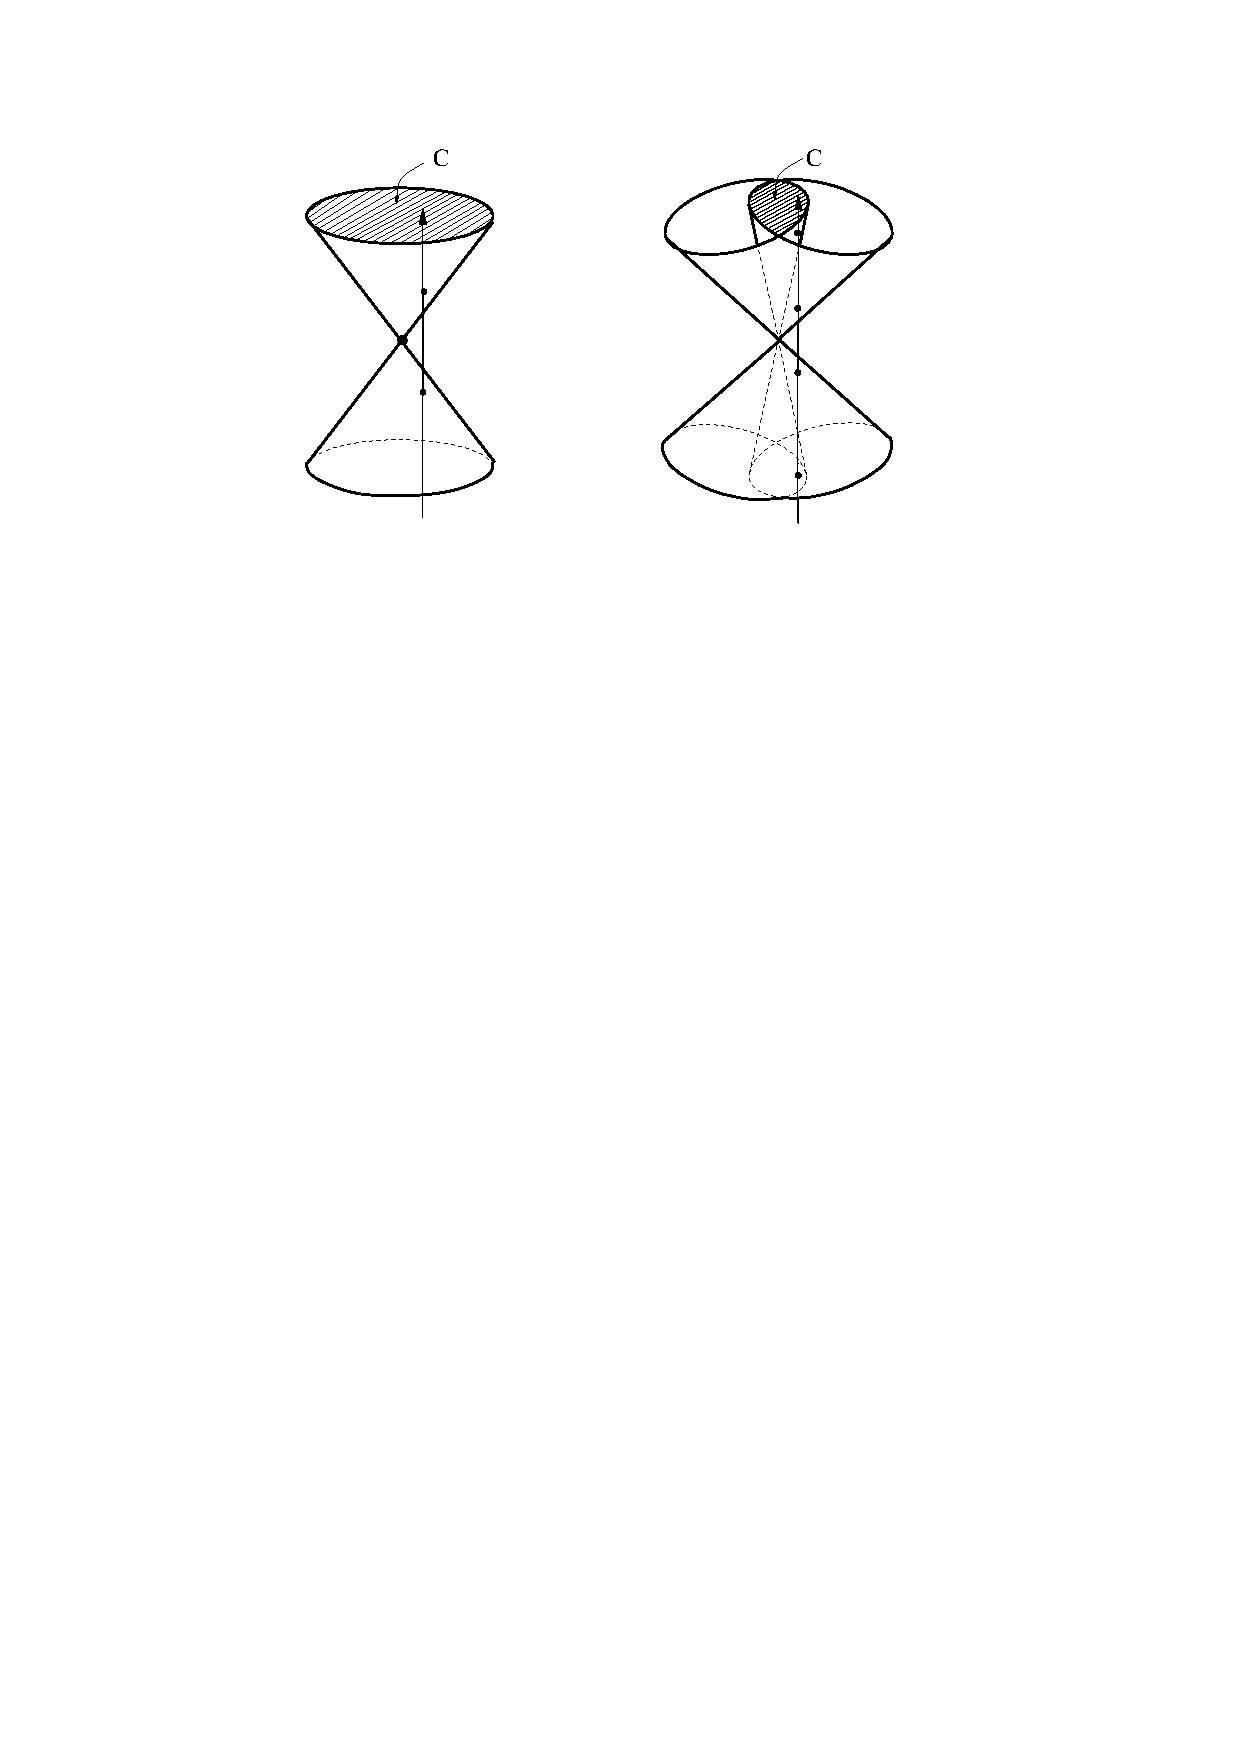
\includegraphics[width=0.8\textwidth]{Poly.pdf}
    \caption{Hyperbolicity cone $C_p$ and vanishing set $V_p$ of a second and a fourth degree polynomial taken from \cite{Rivera}.}
    \label{hyperbol}
\end{figure}
One can now see the underlying geometric interpretation hyperbolic covectors for a given polynomial. If $\mathcal{P}_p$ is hyperbolic w.r.t. $h$ than any affine line in direction $h$ intersects $\mathrm{deg}(\mathcal{P}_p)$ times with the vanishing set $V_p(\mathcal{P}_p)$.
Finally we can state the connection between hyperbolic polynomials and the well posedness of the Cauchy problem.
\begin{theorem}
If a given PDE is well posed in a region of $M$ than the principal polynomial restricts to a hyperbolic polynomial $\mathcal{P}_p$ at every $p$ in that region. Furthermore at $p \in M$ exactly those hypersurface containing $p$ and having a conormal vector that is hyperbolic w.r.t. $\mathcal{P}_p$ are suitable \textit{\textbf{initial data hypersurfaces}}, i.e. yield a well posed Cauchy problem.
\end{theorem}
\begin{proof}
The proof can be found in \cite{Hormander1977} and \cite{Ivrii_1974}.
\end{proof}
Hence we can sum up the situation as follows: If we have given a predictive PDE in the sense that there exist hypersurfaces such that the corresponding Cauchy problem is well posed, then we can calculate the principal polynomial of this PDE. This principal polynomial is then necessarily a hyperbolic polynomial when restricted to the appropriate points $p \in M$. As shown above the zero variety of the principal polynomial describes the propagation of waves in the infinite frequency limit. Furthermore from the principal polynomial we can compute the hyperbolicity cones. These then precisely encode the admissible initial data hypersurface of the given PDE.\\ 

The above consideration immediately opens up a problem that we are going to outline in the following. in the first section we developed the necessary techniques that allowed us to phrase the requirement of diffeomorphism invariance in terms of a linear, first order PDE. given a concrete space time geometry in terms of a field bundle $F_{grav}$ computing solutions to the corresponding equivariance equation (\ref{DiffeoEqn}) would yield a diffeomorphism invariant theory of gravity in terms of a Lagrangian for the gravitational field and the corresponding gravitational equations of motion.  

On the other hand in order to really put that theory into use and calculate predictions we additionally would need a theory of the matter that couples to that particular gravitational field. In the context of constructive gravity usually one even assumes that the matter theory is given first according to some phenomenological observation and one then tries to construct a compatible theory of gravity. In either case we get additional to the gravitational EOM a set of matter EOM.

More precisely the situation now looks as folllows.
The gravitational Lagrangian is given by a bundle map 
\begin{align}
    \mathcal{L}_{grav} : J^2F_{grav} \longrightarrow \Lambda^4M
\end{align}
where $F_{grav}$ is the gravitational field bundle. Additionally we now also have a matter field described by a Lagrangian that depends on the values of the matter field, its first derivatives\footnote{We might also here consider the case where the Lagrangian also depends on second derivatives of the matter field and is thus required to be degenerate s.t. the matter EOM are again of second derivative order but for simplicity we restrict to first order matter Lagrangians.} but also exploits the spacetime geometry provided by the gravitational field. Thus the matter Lagrangian is bundle map
\begin{align}
    \mathcal{L}_{mat} : F_{grav} \times J^1F_{mat} \longrightarrow \Lambda^4M,
\end{align}
where $F_{mat}$ is the matter field bundle. In the following we will denote adapted coordinates on $J^1F_{mat}$ by $(x^m,\phi^{\tilde{A}},\phi^{\tilde{A}}_m)$ Hence the total Lagrangian is given by:
\begin{align}
\begin{aligned}
    \mathcal{L}_{tot} : &J^2F_{grav} \times J^1F_{mat} \longrightarrow \Lambda^4M \\
    &\mathcal{L}_{tot} = \mathcal{L}_{grav} + \mathcal{L}_{mat}.
\end{aligned}
\end{align}
We now get two sets of EOM one from taking the variational derivative of $\mathcal{L}_{tot}$ w.r.t the gravitational field bundle coordinates, i.e. the gravitational EOM and one from taking the variational deriavtive w.r.t. the matter field bundle coordinates $\phi^{\tilde{A}}$, the matter EOM.
The gravitational EOM now feature an inhomogeneous terms that describes how the gravitational field is sourced by the matter.
\begin{align}
    0 = \frac{\delta \mathcal{L}_{tot}}{\delta v_A} = \frac{\delta \mathcal{L}_{grav}}{\delta v_A} + \frac{\delta \mathcal{L}_{mat}}{\delta v_A}.
\end{align}
The matter EOM is given by 
\begin{align}
    0 = \frac{\delta \mathcal{L}_{mat}}{\delta \phi^{\tilde{A}}}.
\end{align}
We can then compute the two principal polynomials that correspond to the two EOMs, $\mathcal{P}_{grav}$ and $\mathcal{P}_{mat}$. Note in particular that these will depend both on the values of the gravitational field. We denote the corresponding vanishing sets by $V_{p,grav}$ and $V_{p,mat}$. As we require both theories to be predictive, i.e. have well posed Cauchy problems we can also compute the two hyperbolicity cones $C_{p,grav}$ and $C_{p,mat}$ that at each spacetime point $p\in M$ encode the possible choices of initial data hypersurfaces for the two theories. 

Doing this at given $p \in M$ we would now end up with one of the following three situations of which we will show in the following only one can serve the purpose of describing a meaningful physical theory:
%3 possible situations
%add figures here ???
\begin{itemize}
    \item $C_{p,grav} \neq C_{p,mat}$ and $V_{p,grav} \neq V_{p,mat}$
    
This situation obviously incorporates the special case where the two hyperbolicity cones are disjoint. This case can be immediately ruled out as then there would not exist a single initial data hypersurface that is common to both theories and hence could serve as a starting point for solving the coupled matter gravity system.   

Also if the two hyperbolicity cones are not disjoint but nevertheless do not coincide we immediately get problems. Then we would either find a suitable matter initial data hypersurface that is no admissible initial data hypersurface for the gravitational EOM, or vice versa we would find a gravitational initial data hypersurface that could not serve for specifying the initial data for the matter EOM. As it can be seen for instance in \cite{Rivera} and \cite{2011PhRvD..83d4047R} the hyperbolicity cone of a given EOM is in close relation with feasible observer definitions for the underlying theory. Any physical meaningful observer must be able to collect data in his spatial surrounding and use the EOM provided by the theory to evolve this initial data to future values and thereby make physical predictions. To allow for this process the spatial surrounding of any possible observer must serve as initial data hypersurface. Hence if there exist initial data hypersurfaces that are exclusive to either the matter or the gravitational EOM we would end up with certain observers that are limited to one of the two theories. Such observers could in particular meaningfully measure data and predict processes in the corresponding free theory, being either the matter theory or gravity, but become meaningless once the coupled case is concerned.

In the following we want to restrict to situations that allow for a unified observer definition, i.e. the observers of gravity and matter theory obey the same laws and in particular posses the same properties no matter if the two theories are coupled or one considers the case of a free treatment of either one independently. Hence we discharge the case where $C_{p,grav} \neq C_{p,mat}$.

\item $C_{p,grav} = C_{p,mat}$ and $V_{p,grav} \neq V_{p,mat}$ 

For this case all initial data hypersurfaces are common to both theories. Nevertheless the vanishing sets of the two principal polynomials differ. We have seen that these vanishing sets govern the propagation behaviour of wave like solutions in the infinite frequency limit. It might hence be possible that if $V_{p,grav} \neq V_{p,mat}$ the wave propagation of matter waves and gravitational waves shows quite different properties. The structure provided by the vanishing sets of the two principal polynomials in particular governs the information regarding future domains that such a propagating wave might causally influence. Doing so it particular encodes the speed of such waves. 

With the recent detection of gravitational waves \cite{2017ApJ...848L..12A}, \cite{2017PhRvL.119n1101A} and \cite{2016PhRvL.116f1102A} also further insight regarding their propagating speed is gained rapidly. 
To provide an example using the observed time difference between the gravitational wave event GW170817 and the gamma ray burst GRB 170817A emitted by a Binary Neutron Star Merger the propagation speed of gravitational waves has already be constrained to deviate not more than $-3\cdot 10^{{-}15}c$ and $+7\cdot 10^{{-}16}c$ from the speed of light $c$ (see \cite{2017ApJ...848L..13A}). Hence it seems reasonable to additionally require that $V_{p,grav} = V_{p,mat}$ to incorporate the thus already observed similarities in the propagation of gravitational and matter waves into our framework. We are hence left with the final option.
\item $C_{p,grav} = C_{p,mat}$ and $V_{p,grav} = V_{p,mat}$ 

This is the only option left and henceforth precisely what we will require in the following. Not only all possible initial value hypersurfaces and therefore all possible observers of the matter and gravity EOM then coincide, this option also requires that the causal structure in the form of wave propagation in the infinte frequency limit is the same for the two theories.  
\end{itemize}
The previous investigation yields the second and last requirement that we wish to pose on the theory of gravity that we want to construct. We require that given a matter theory that employs the theory of gravity as geometric background, the two theories are \textit{\textbf{compatible}} in their \textit{\textbf{causal structure}} in the sense that the two principal polynomials at each point yield the same vanishing set, i.e. it holds for all $p \in M$ that: 
\begin{align}
    V_{p,grav} = V_{p,mat}.
\end{align}
Note that then $C_{p,grav} = C_{p,mat}$ immediately follows. Further note that as  here we are working with vanishing sets of individual polynomials the above condition simply requires the two polynomials to be compromised of the same irreducible polynomial factors. In most relevant cases the factorization of the polynomials can easily be obtained. In other words here we do not need to work with the polynomial ideals that vanish on the respective sets and hence do not need further techniques from algebraic geometry such as Gröbner basis that allow for efficiently deciding whether or not a given polynomial lies inside such an ideal and hence vanishes on the corresponding set.  
%remove last statement

Summing up the previous achievements it is now conceptually completely clear how we must proceed to find the most general gravitational lagrangian that is compatible with any given matter theory. We first solve the equivariance equations (\ref{DiffeoEqn}) to implement the required diffeomorphism invariance of the theory of gravity paying close attention to make sure that the resulting EOM are of no higher than second derivative order. Then we compute the gravitational principal polynomial and compare it to the one obtained from the matter theory. We require that at each spacetime point the two polynomials define the same vanishing set and by this get further conditions the gravitational lagrangian has to solve, this time encoding the causal compatibility between matter theory and gravity.\\

We end this section by reformulating the previous results in terms of a definite construction recipe that is displayed as Algorithm (\ref{Algo1}).
\begin{algorithm}[ht]
\SetAlgoLined
\KwData{Matter theory $ \mathcal{L}_{mat} : F_{grav} \times J^1F_{mat} \rightarrow \Lambda^4M$
}
\KwResult{Most general diffeomorphism invariant, causal compatible $\mathcal{L}_{grav} : J^2F_{grav} \rightarrow \Lambda^4M$ }
Compute the constant tensors $C^{Bm}_{An}$ \\
Set up the equivariance equations (\ref{DiffeoEqn}) \\
Solve the equivariance equations (\ref{DiffeoEqn}) to obtain the most general $L_{grav}(x^m,v_A,v_{Am},v_{AI})$\\
Compute the EOM $\frac{\delta L_{grav}}{\delta v_A}$\\
Consider the most general subtheory that has 2nd order EOM\\
Calculate the principal polynomials $\mathcal{P}_{grav}$ and $\mathcal{P}_{mat}$\\
Determine the arbitrary quantities in $L_{grav}$ s.t. for all $p \in M$ : $V_{p,grav} = V_{p,mat}$
 \caption{Construction of Gravitational Lagrangian}\label{Algo1}
\end{algorithm}
\section{Perturbative Approach to Constructive Gravity}
In the previous section we have completed the required diffeomorphism invariance of the gravitational theory with the second requirement $V_{p,grav}=V_{p,mat}$ ensuring the compatibillity with a given matter theory. In principal it is therefore entirely clear how one can solve the problem posed by constructive gravity. Practically obtaining solutions to the diffeomorphism equivariance equations (\ref{DiffeoEqn}) is however a different question. Although the relevant PDE is linear in the unknown Lagrangian and furthermore only of first derivative order --- methods for solving  such PDEs have actually already been known for a long time \cite{Han2015} --- already treating the standard case of finding the most general such Lagrangian that can be constructed from a metric tensorfield and its first and second derivatives is surprisingly hard. The reason is the shear size of the resulting pde system. For the stated example we will later see that the PDE system is compromised of a total of 136 partial differential equations and the Lagrangian is a function of 150 independent variables.  

Regarding this we are essentially left with one of two options that avoid the mammoth task of solving the equivariance equations in fully general form and nevertheless furnish us with access to two exeptionally relevant realms of gravitational physics. We can either apply \textbf{\textit{symmetry}} methods to the equivariance equations and thereby for a given gravitational field obtain solutions, i.e. theories of gravity that describe the relevant phenomenology under these symmetry assumptions. We could for instance solve the equations for spatial homogenity and isotropy to obtain a description of cosmology in the generalised spacetime geometry. Alternatively --- and this is the path that we will take in the following --- we can perturbatively solve the equivarinace equations by means of a \textit{\textbf{power series solution}} to some finite order. We in particular chose this path with the treatment of gravitational waves in mind.  The recent developments in the dectection of gravitational waves makes them an excellent tool to test alternatives to GR \cite{2010PhRvD..81f4008Y}, \cite{2011PhRvD..83j4022B}, \cite{2017PhRvD..95j4027Z}, \cite{2013LRR....16....9Y}. \\

We have already gathered the necessary techniques that allow us to construct perturbative solutions to the equivariance equations in a rigorous fashion in the previous section. primarly we have seen that such an approach only yields meaningful results if the relevant PDE is \textit{\textbf{involutive}}. We are now going to apply these technniques to the equivariance equations (\ref{DiffeoEqn}). To that end it is important to take a closer look at the jet bundle that underlies the  geometric treatment of the PDE provided by (\ref{DiffeoEqn}). Recall that the lagrangian was given by a bundle map 
\begin{align}
\mathcal{L} : J^2F \longrightarrow \Gamma^4M.
\end{align}
Abstractly the PDE (\ref{DiffeoEqn}) is then given as a submanifold of the first order jet bundle $J^1(J^2F \times \Lambda^4M)$ over the trivial bundle $J^2F \times \Lambda^4M$. 
We can denote adapted coordinates on $J^1(J^2F \times \Lambda^4M)$ by $(x^m,v_A,v_{Am},v_{AI},l,l^{m},l^{A},l^{Am},l^{AI})$ such that we could obtain the formal representation of the PDE (\ref{DiffeoEqn}) by replacing the bundle map $L$ the derivatives $L^{:m},L^{:A},...$ with fibre coordinates $l$ and derivative coordinates $l^m,l^A,...$. Hence in terms of formal PDE theory the equivariance equation reads 
\begin{align}\label{DiffeoEqnFormal}
\begin{aligned}
    0 &= l^{m} \\
    0 &= l^{A} C_{An}^{Bm} v_B + l^{Ap} \bigl[ C_{An}^{Bm} \delta_p^q - \delta_A^B \delta_m^n \bigr] v_{Bq} + l^{AI} \bigl[ C_{An}^{Bm} \delta_I^J - 2 \delta_A^B J_I^{pm} I^J_{pn}  \bigr] v_{BJ} + l \delta^m_n \\
    0 &= l^{A(p\vert}C_{An}^{B \vert m)} v_B + l^{ AI} \bigl[ C_{An}^{B(m\vert} 2 J_I^{\vert p) q} - \delta^B_A J_I ^{pm} \delta_n^q \bigr] v_{Bq} \\
    0 &= l^{AI} C_{An}^{B(m\vert} v_B J_I^{\vert p q )}.
    \end{aligned}
\end{align}

We begin the perturbative treatment of constructive gravity with one of the main results that in the end justifies the perturbative approach:
\begin{theorem}
PDE (\ref{DiffeoEqnFormal}) is involutive.
\end{theorem}
\begin{proof}
We start by proofing that the symbol of the equation (\ref{DiffeoEqnFormal}) is involutive. Due to the fact that the PDE is of first derivative order it symbol simply consists of its homogeneous part, namely the PDE with the second equation being replaced by the homogeneous counterpart:
\begin{align}
    0 &= l^{A} C_{An}^{Bm} v_B + l^{Ap} \bigl[ C_{An}^{Bm} \delta_p^q - \delta_A^B \delta_m^n \bigr] v_{Bq} + l^{AI} \bigl[ C_{An}^{Bm} \delta_I^J - 2 \delta_A^B J_I^{pm} I^J_{pn}  \bigr] v_{BJ}.
\end{align}
This homogeneous system describes functions that are invariant under the action of any lifted vector field (\ref{LieJ2}). 

The first step in proving involution of the symbol is computing the sum of beta numbers. We have to pay attention as we have to compute this sum in coordinates that maximize it, i.e. are $\delta$-regular. However due to the fact that we are dealing with first order equations the classes of the derivative indices all posses exactly one member and range from 1 to $\mathcal{k}$ where 
\begin{align}
    \mathcal{k} := \mathrm{dim}(J^2F) = 4+n+4n+10n.
\end{align}
In the following we are going to assume that $\mathrm{dim}(J^2F)$ is bigger than the number of independent equations in (\ref{DiffeoEqnFormal}) which is given by 140 as otherwise in general there will not exist solutions in the first place. 
The maximum value for the sum of betas is obtained when we transform the coordinates on $J^2F$ s.t. the first equation is solved w.r.t. the derivative coordinate with class $\mathcal{k}-140+1$ and the $i$-th equation is solved w.r.t. the derivative coordinate of class $\mathcal{k}-140+i$ such that the last equation is solved w.r.t. the derivative coordinate of maximum class $\mathcal{k}$. If we display the symbol $M_1$ as matrix and label its columns by class starting from 1 and its rows from 1 to 140 this transformation this coordinate transformation on $J^2F$ corresponds to bringing the matrix to the following upper triangular form
\begin{align}\label{symbolMat}
\begin{bmatrix} 
      0 & \hdots & 0 & 1 & a_{1,1} & \hdots & \hdots & a_{1,139} \\
      \vdots &  & \vdots & 0 & \ddots & \ddots & & \vdots  \\
      \vdots & & \vdots & \vdots & \ddots  & 1 & \ddots & \vdots  \\
      \vdots & & \vdots & \vdots & & \ddots & \ddots & a_{139,139} \\
      0 & \hdots & 0 & 0 & \hdots  & \hdots & 0 & 1
\end{bmatrix}
\end{align}
for some $a_{i,j}$ that are functions on $J^2F$ . The sum of betas can then be computed to be given by:
\begin{align}
    \sum_{i=1}^{\mathcal{k}} i \beta_1(i) = \sum_{i = 1}^{140} \mathcal{k} -140+i.
\end{align}
We now have to show that this equals the rank of the prolonged symbol $M_2$. By previous arguments this is the case if we obtain all equations of order 2 by prolongation w.r.t. multiplicative variables only. We again consider the symbol solved to the form given by matrix (\ref{symbolMat}). 
To simplify the notation in the following we denote coordinates on $J^2F$ that bring the symbol to this form by $y_a$ for $a = 1,...,\mathcal{k}$. Note that such coordinates always exist. We take an arbitrary row $\sigma$ from the matrix (\ref{symbolMat}) for $\sigma=1,...,140$ and then consider the corresponding equation $E_{\sigma}$. The multiplicative variables of this $\sigma$-th equation are $y_1,...,y_{\mathcal{k}(\sigma)}$ where we introduced 
\begin{align}
\mathcal{k}(\sigma):= \mathcal{k} -140 + \sigma.
\end{align}
We now show that prolonging this equation w.r.t. an arbitrary non multiplicative variable $y_b$ for $b>\mathcal{k}(\sigma)$ yields no additional independent contribution to the prolonged symbol. This is achieved by showing that we can add prolongations w.r.t. multiplicative variables to such a non multiplicative prolongation $D_bE_{\sigma}$ and thereby obtain an equation of first derivative order which is thus not present in $M_2$. Note that in the matrix (\ref{symbolMat}) multiplicative variables of a given row are exactly those corresponding to the columns that are left to the pivots $1$ (including these) and contain zeros and non multiplicative variable correspond to the columns right to the pivots and hence contain the $a_{i,j}$. Prolonging $E_{\sigma}$ w.r.t. such a $y_b$, i.e. computing $D_bE_{\sigma}$ we get second order derivatives of the form $y_{bc}$ for $c > \mathcal{k}(\sigma) $. For these derivatives there are now essentially two possibilities, either $b<c$ then we can get rid of this contribution by considering the equation with leading derivative, i.e. lowest ranked derivative $y_c$. This is precisely equation $E_{\mathcal{k}^{-1}(c)}$. We prolong this equation w.r.t. $y_b$. As $b<c$ this prolongation is now multiplicative. We then subtracting this multiplicative prolongation from $D_bE_{\sigma}$ to remove this second derivative order contribution $y_{bc}$.

Consider now the case where $c<b$. We then simply apply the procedure the other way round. We take equation $E_{\mathcal{k}^{-1}(b)}$, apply the multiplicative prolongation w.r.t. $y_c$ and subtract the result $D_cE_{\mathcal{k}^{-1}(b)}$ from the original prolongation. Doing this we can remove all second order derivatives from the non multiplicative prolongation $D_bE_{\sigma}$ by subtracting  multiplicative prolongations $D_bE_{\mathcal{k}^{-1}(c)}$ or $D_cE_{\mathcal{k}^{-1}(b)}$. Hence any non multiplicative prolongation does not contribute an independent new second derivative order equation to the prolonged symbol $M_2$ and the symbol. The symbol is therefore involutive. 

In order to proof that not only the symbol but also the PDE (\ref{DiffeoEqnFormal}) itself involutive we have to show that the PDE generates no integrability conditions after one prolongation. We have already discussed that prolonging each equation only w.r.t. its multiplicative variables never produces integrability conditions. Furthermore we have just shown that any prolongation w.r.t. non multiplicative variables can be reduced to first derivative order by adding further multiplicative prolongations in the way it is outlined above. Hence the question is if the first derivative order contributions that we get from such a procedure are already included in $R_1$ or contribute additional independent equations. 

We first consider the homogeneous case. We take again the m-th equation and work as before in the coordinates $y^a$ on $J^2F$ that solve the symbol $M_1$ to (\ref{symbolMat}). Note that this homogeneous linear first order PDE can then be concisely written as
\begin{align}
    E_{\sigma} = l_{\mathcal{k}(\sigma)} + \sum_{i = 1}^{140-\sigma} a_{\sigma,i} l_{\mathcal{k}(\sigma)+i} .
\end{align}
We can equivalently write this in the form of vector fields on $J^2F$. We define for $\sigma = 1..140$ the vector fields $\zeta_{\sigma} \in \Gamma(J^2F) $ corresponding to $E_{\sigma}$:
\begin{align}
    \zeta_{\sigma} := \frac{\partial}{\partial y_{\mathcal{k}(\sigma})} + \sum_{i = 1}^{140-\sigma} a_{\sigma,i} \frac{\partial}{\partial y_{\mathcal{k}(\sigma)+i}}.
\end{align}
The solutions to the given homogeneous PDE are then precisely those functions on $J^2F$ that are invariant under these vector fields, i.e. that satisfy $\zeta_{\sigma} f = 0$ for all values of $\sigma$.
Note that we obtained the homogeneos PDE from precisely such an invariance requirement. The only difference to the previous case is that we now work coordinates that render the symbol particularly simple. 
In terms of vector fields this corresponds to the fact that the $\zeta_{\sigma}$ commute (see also \cite{seiler1994analysis}).
%136 vs 140 !!!
%
%
%

Carefully analysing the above procedure we now find that the remaining first order equation that is produced when eliminating all second order contributions of a non multiplicative prolongation $D_bE_{\sigma}$ by multiplicative prolongations is simply given by the commutator equation
\begin{align}
    \left [\zeta_{\sigma}, \zeta_{\mathcal{k}^{-1}(b)} \right] = 0.
\end{align}
Hence for the system to not produce integrability conditions this commutator must now be given by a linear combination of unprolonged equations. For the particular case of the $\zeta_{\Sigma}$ this is trivially true as the commutator of two such fields vanishes. This can however already be seen from the original system (\ref{DiffeoEqnFormal}).
Recalling that we obtained homogeneous counterpart to (\ref{DiffeoEqnFormal}) by requiring invariance under the prolonged vector fields $\xi_{J^2F}$ (\ref{LieJ2}) that were in particular constructed via a Lie algebra morphism. It is therefore clear that also these vector fields close under the operation of taking commutators. Hence no integrability conditions are generated and the homogeneous system is involutive.

This is no special property of the homogeneous PDE in consideration but is actually general to all linear homogeneous first order PDEs. Such PDEs that can be described entirely by vector fields are called \textit{\textbf{complete}} if the vector fields that generate the given system form a Lie algebra w.r.t. the commutator. If the vector fields commute the system is furthermore called a \textit{\textbf{Jacobian}} system. One can show along the same lines that we followed her that in fact any complete system is involutive. For details regarding the treatment of complete systems and in particular for a proof of this last statement see \cite{seiler1994analysis} and also for further information \cite{Clebsch1866}, \cite{caratheodory1956variationsrechnung} and \cite{lie1970theorie}.\\

What remains show is that the presence of the inhomogenity in $(\ref{DiffeoEqnFormal})$ does not change this observation, i.e. does not generate integrability conditions. We again work in the coordinates $y_a$. The inhomogenity is only present in the equations $5-20$ and only when the indices in (\ref{DiffeoEqnFormal}) are such that $m = n$. We label the equations s.t. it contributes to equation $5,9,13$ and $17$. In each case the contribution is simply given by an extra term of $+l$ and the respective equations $\Tilde{E}_{\sigma}$ of the inhomogeneous PDE read now 
\begin{align}
     \tilde{E}_{\sigma} = \begin{cases}
     E_{\sigma} + l \ \text{for} \ \sigma \in \{ 5,9,13,17 \}\\
     E_{\sigma} \ \text{else}.
     \end{cases}
\end{align}
One can now show along the same lines the we followed in the homogeneous case that the inhomogeneous system is involutive if for any two such equations $\tilde{E}_{\sigma}$ and $\tilde{E}_{\tau}$ the so called \textit{\textbf{Jacobi brackets}} or sometimes also called Mayer bracket 
\begin{align}
  \llbracket \tilde{E}_{\sigma}, \tilde{E}_{\tau} \rrbracket = \sum _{i = 1}^{\mathcal{k}} (\frac{\partial \tilde{E}_{\sigma}}{\partial l_i}) D_{i}\tilde{E}_{\tau} -  (\frac{\partial \tilde{E}_{\tau}}{\partial l_i}) D_{i}\tilde{E}_{\sigma} 
\end{align}
vanish on $R_1$ (see  \cite{seiler1994analysis} and also also Example 2.3.12 in \cite{seiler2009involution}), i.e. can be obtained by linear combinations of unprolonged equations. Comparing this to the previous case where the possible integrability conditions where built from the commutator we now get extra terms whenever either $\sigma$, $\tau$ or both are contained in $\{ 5,9,13,17 \}$. Consider first the case where $\sigma \in \{5,9,13,17\}$ but not $\tau$, then we have $\tilde{E}_{\sigma} = E_{\sigma} + l$ and $\tilde{E}_{\tau} = E_{\tau}$ and hence using the linearity of the Jacobi bracket
\begin{align}
    \llbracket \tilde{E}_{\sigma}, \tilde{E}_{\tau} \rrbracket = \llbracket E_{\sigma}, E_{\tau} \rrbracket - \sum_{i=1}^{\mathcal{k}} \frac{\partial E_{\tau}}{\partial l_i} l_i.
\end{align}
We can now use that the first contribution vanishes, $\llbracket E_{\sigma}, E_{\tau} \rrbracket = 0$ as this again essentially nothing different that the commutator of the two vector fields $[\zeta_{\sigma},\zeta_{\tau}]$ expressed in terms of the quantities $E_{\tau}$ and $E_{\sigma}$. We are thus left with the second term $- \sum_{i=1}^{\mathcal{k}} \frac{\partial E_{\tau}}{\partial l_i} l_i$, but as the equation $E_{\tau}$ is in particular linear in the $l_i$ this again yields $E_{\tau}$ and hence vanishes on $R_1$. Along the same lines one can proceed with the case of $E_{\tau}$ also containing extra contributions from $+l$. In total we thus find that also the inhomogeneous PDE is involutive which proofs the statement.
\end{proof}
%check this proof !!!

We can now apply the preveous developed techniques to obtain a power series solution to the PDE (\ref{DiffeoEqnFormal}). This then yields a finite order power series expansion of the requested gravitational Lagrangian of which we can of course compute the Euler Lagrange equations in the appropriate perturbative order. In other words we thus get a perturbative theory of gravity. We consider the result that the PDE (\ref{DiffeoEqnFormal}) is involutive to be essential for this approach as only now as we have proven that we can be sure the contribution to the perturbative Lagrangian that we compute up to some finite order will not change in any higher order of the power series procedure. Differently stated only with the PDE being involutive we can be certain to  really extract all the for the particular order relevant information from it and not end up with a solution that is too general. \\

Note that from the point of view of formal theory involution of a PDE is not only essential for the construction of power series solution. Previously we have already stated that one of the key ideas behind a PDE with involutive symbol lies in the fact that one is then able to predict the rank of the prolonged symbol by means of (\ref{sumBeta}) without actually having to compute the relevant prolongations. As for an involutive symbol according to (\ref{invoCons}) also all prolonged symbols are involutive one can thus obtain formulae that also allow for the prediction of the ranks of higher order prolongations of the symbol. Recall that the rank of the symbol $M_q$ essentially determines the number of expansion constants of order q the one might specify arbitrarily when constructing a power series solution to the PDE  and thereby the various ranks of the symbol govern the entire information regarding the solution space of the given PDE.
Thus the involution of the PDE (\ref{DiffeoEqnFormal}) allows us to formulate the following statement about its general solution for arbitrary field bundles $F$.
\begin{theorem}\label{GeneralSol}
Given any field bundle $F$ with fibre dimension $n$. The general solution to the invariance equation, i.e. the homogeneous version of (\ref{DiffeoEqnFormal}) admits the form:
\begin{align}
    \mathcal{F} \left (\Psi_1,...,\Psi_r \right ),
\end{align}
where $r:=\mathcal{k}-140$, $\Psi_1,...\Psi_r$ are $r$ funtionally independent solutions of the homogeneous PDE and $\mathcal{F}$ is an arbitrary function of these independent solutions. The general solution to the equivariance equation, i.e. the inhomogeneous PDE (\ref{DiffeoEqnFormal}) is given by:
\begin{align}
    \omega \cdot \mathcal{F} \left (\Psi_1,...,\Psi_r \right ),
\end{align}
where $\omega$ is any explicit solution of the PDE. 
\end{theorem}
\begin{proof}
The proof of the first statement is given by Proposition 7.1 in \cite{seiler1994analysis}. Further information can in particular be found in chapter 3 of \cite{seiler2009involution} and \cite{articleCH}. 

The second statement then simply follows from the previously stated fact that given an arbitrary solution $\mathcal{F}$ of the homogeneous PDE, multiplying by any solution $\omega$ of the inhomogeneous system yields again a solution of the inhomogeneous system and vice versa the quotient of any two solutions of the inhomogeneous PDE defines again a solution of the homogeneous system. The first part of this statement is simply a result of the linearity of the given PDE. For simplicity we consider the case of a single equation 
\begin{align}
    0=D_i l + l 
\end{align}
and the corresponding homogeneous version. The generalization to finitely many equations is then realy straight forward. 
We thus have $0 = D_i \mathcal{F}$ and also $0 = D_i \omega + \omega$.
We first show that $\omega \cdot \mathcal{F}$ then also solves the inhomogeneous system. Inserting $\omega \cdot \mathcal{F}$ into the inhomogeneous PDE we get 
\begin{align}
    0 = \left ( D_i \mathcal{F} \right ) \cdot \omega + \mathcal{F} \cdot \left ( D_i \omega \right) + \mathcal{F} \cdot \omega. 
\end{align}
As $\mathcal{F}$ is supposed to provide a solution of the homogeneous equation the first term vanishes. As $\omega$ solves the inhomogeneous equation the second term yields $\mathcal{F} \cdot \left ( - \omega \right )$,
and thus cancels the third term. We thus have shown that $\omega \cdot \mathcal{F}$ solves the inhomogeneous system. To complete the proof we still have to show that any solution of the inhomogeneious PDE is neccessary of this form. We proof this by first taking an arbitrary solution of the inhomogeneous system $\rho$. We now take any other solution $\omega$ and insert the quotient $\frac{\rho}{\omega}$ into the homogeneous PDE
\begin{align}
    0 = D_i \left (\frac{\rho}{\omega} \right) = - (\frac{\rho}{\omega}) - \frac{\rho}{\omega^2} \cdot (-\omega) ,
\end{align}
where we used $D_i \rho = -\rho$ and the same for $\omega$ as they both are supposed to solve the inhomogeneous system. Hence the quotient solves the homogeneous system. Obviously we can write the solution $\rho$ as 
\begin{align}
    \rho = \omega \cdot  \frac{\rho}{\omega}.
\end{align}
But as the first factor is taken to be a solution of the inhomogeneous system and we have now shown that the second factor solves the homogeneous PDE this is precisle the form that was claimed. 
Hence in total we have thus shown that any solution of the inhomogeneous PDE is of the form $\omega \cdot \mathcal{F}$.
The straight forward generalization of this to the case finitely many PDEs then completes the proof.
\end{proof}
It is important to observe that the previous theorem not only tells us the generall form any solution to the equivariance or invariance equations respectively will admit but also provides us with information regarding the number of functionally independent solutions to these systems. Concretely for any field bundle there will be 
\begin{align}
    \mathcal{k} - 140 = \mathrm{dim}(J^2F)
\end{align}
functionally independent solution. This is obviously something that one might intuitively guess as it is simply the difference between the number of independent variables in $J^2F$ and the number of equations in the PDE. However only now that we know the equations are involutive we can be sure that there is no further information hidden in them yielding possibly additional restrictions on the unknowns and thereby reducing the number of functionally independent solutions. 
Also note that these solutions now in general will correspond to Lagrangians that might generate 4-th derivative order EOM. 
In the context of GR these functionally independent solutions of the homogeneous equations are called \textit{\textbf{curvature invariants}}. In most cases they are constructed form the Riemann curvature tensor. Observe however that also her the Riemann curvature is strictly speaking not necessary to obey such a notion of curvature invariants. 
In GR it is a well known result that there exist 14 functionally independent curvature invariant, yet already for this rather simply case their concrete expressions is surprisingly difficult. Obtaining possible generating sets that allow one to express arbitrary other invariants in terms of them is still a topic of research. The curvature invariants and also possibly higher invariants involving higher derivatives of the metric tensor are then mostly used to classify spacetimes. Details can be found in
\cite{2009CQGra..26b5013C}, \cite{Zakhary1997}, \cite{2002IJMPD..11..827C} and also \cite{doi:10.1063/1.531425}.
Note that we can easily reproduce the known result of 14 curvature invariants for GR in our framework. The fibre dimension of the bundle of symmetric $(0,2)$ tensors $F_{GR}$ is obviously 10 yielding for this case 
\begin{align}
    \mathrm{dim}(J^2F_{GR}) = 4 + 10 + 40 + 100 = 154,
\end{align}
which according to the above considerations yields $154-140=14$ functionally invariant solutions. Beyond the standard case of GR we are know in a position where we can easily determine the number of curvature invariants for any other spacetime geometry. We will consider a particular example in the next chapter.\\ 

Before we concretely work out a general framework for obtaining perturbative solutions to the equivariance equations we concern ourselves for a moment with the question what points $p_0 \in J^2F$ might serve the purpose as expansion points for such a power series. From the shear mathematical point of view there is really no restriction on the possible expansion points. Yet from a physical point of view the specific expansion point will in the end determine the interpretation and foremost the range of validity of the thereby constructed perturbative theory of gravity. As we want to work towards a treatment of gravitational waves we are going to restrict ourselves to certain expansion points that describe a \textit{\textbf{flat}} variant of the theory of gravity at hand. Solutions of the obtained perturbative equations can then be thought of as corrections to that flat background theory with the special case of gravitational waves being wave like solutions that propagate on the given background. More precisely with a slight adaption of the usual meaning in Riemanian geometry\footnote{In Riemannian geoemtry one call a Riemannian manifold flat if the associated Riemannian curvature tensor vanishes everywhere. The existance of coordinates for which the derivatives of the metric are zero is then a consequence (see \cite{petersen2006riemannian}).} we call a section $G \in \Gamma(J^2F)$ \textit{\textbf{flat}} if there exist adapted coordinates on $J^2F$ s.t. the coordinate expression of $G$ satisfies $\partial_mG_{A}=0$.
Hence we chose an expansion point with adapted coordinates $(x_0^m,N_A,0,0)$. note that such a point is essentially already determined by a point in $F$. 

We are in particular interested in the case where the expansion point is not only flat but furthermore supports our intuition that the geometry of spacetime is in quite good approximation provided by the flat Minkowski metric $\eta_{ab} = \mathrm{diag}(-1,+1,+1,+1)$. 
%check signature !!!
%
%
In other words we want to interpret solutions of the to-be-constructed perturbative theory of gravity as corrections to a flat Minkowski background. Note we are not restricting our treatment to metric theories of gravity but deliberately want to allow for more general tensor fields as spacetime geometry.
The interpretation of doing perturbation theory around Minkowski spacetime will nevertheless become meaningful once the additional matter theory $\mathcal{S}_{mat}[\phi^{\tilde{B}},G_A)$ is provided. We then require from our flat expansion point that the matter theory obtained from this flat expansion background $\mathcal{S}_{mat}[\phi^{\tilde{B}},N_A)$ is equivalent to the counterpart that we get when placing the matter field $\phi^{\tilde{B}}$ on a Minkowski background. 
In most cases this is achieved by constructing $N_A = N_A(\eta_{ab})$ from the Minkowski metric. We call such expansion points in the following \textit{\textbf{$\boldsymbol{\eta}$-induced}}. Note that this clearly restricts the set of field bundles $F$ we can possibly treat to those that are compromised of tensors with an even total rank, as we simply cannot write down expressions with odd rank that are solely constructed from $\eta_{ab}$. This will not affect any further developements as in all examples we will treat, the gravitational field is described by an even rank tensor field. There are even certain arguments mainly stemming from QFT that the gravitational field must be of even rank in order to describe an attractive force (\cite{vecchiato2017variational}). \\

We start our development of a framework that will allow us to construct perturbative expansions of diffeomorphism invariant Lagrangians for arbitrary fields by writing down the general finite power series expansion of an arbitrary such Lagrangian up to some order $r > 0$ around a flat expansion point $p_0 \in J^2F$ with adapted coordinates $p_0 \equiv (x_0^m,N_A, 0, 0)$ . Note again that such a Lagrangian is already a bundle map on the second order jet bundle $J^2F$, the equivariance PDE (\ref{DiffeoEqnFormal}) is then constructed as submanifold of $J^1(J^2F \times \Lambda^4M)$. It is important to not confuse the two different ways the jetbundle construction is involved therein. In order to concisely display such a power series Lagrangian we need to agree on some further notation. We denote the adapted coordinates on $J^2F$ collectively by
\begin{align}
    (v_{AI_k}) := (x^m,v_A,v_{Ap},v_{AI}).
\end{align}
In order to distinguish the appearing derivative indices $I_k,J_k,...$ that label higher spacetime derivatives from those that label higher derivatives w.r.t. the coordinates of $J^2F$ we denote the latter ones by caligraphic letters
%add this to introduction !!!
$\mathcal{I}_k, \mathcal{J}_k$, ... . Finally we introduce the coordinate expression of the deviation from the expansion point 
\begin{align}
    (H_{AI_k}) := (v_{AI_k}) - (N_{AI_k}) = (x^m-x_0^m,v_A-N_A,v_{Ap},v_{AI}).
\end{align}

Before we write down the concrete expression for the expansion of the Lagrangian note that the first equation in (\ref{DiffeoEqnFormal}) simply states that the Lagrangian must not explicitly depend on $x^m$, hence we can discharge any explicit $x^m$ dependency from the very beginning and therefore also exclude such from the power series expansion. In total with the introduced notation a general power series expansion reads as follows. 
\begin{align} \label{generalPowerSL}
    \begin{aligned}
    &L_{per} \cdot  \mathrm{d}^4x = \mathcal{L}_{per} : J^2F \longrightarrow \Lambda^4M \\
    &L_{per} = \sum_{n=0}^r \sum_{k_1,...,k_n = 0}^2 a^{\mathcal{I}_k} \cdot J_{\mathcal{I}_k}^{A_1I_{k_1}...A_nI_{k_n}} H_{A_1I_{k_1}} \cdot ... \cdot H_{A_nI_{k_n}}
    \end{aligned}
\end{align}
%rewrite this ???
%
%
As before the $a^{\mathcal{I}_k} =: a^{A_1I_{k_1}...A_nI_{k_n}}$ are constants. 
In order to clarify this last expression further we now explicitly provide the first three orders of this expansion. For that particular case we drop any numerical factors due to the intertwiners as this simply corresponds to redefining the constants. Furthermore as before we are going to split the sums over the ${A_iI_{k_i}}$ into the different contributions $(v_A,v_{Ap},v_{AI})$:
\begin{multline}\label{LPert}
    L_{per} = a_0 + a^A H_A + a^{Ap} H_{Ap} + a^{AI}H_{AI} + a^{AB} H_{A}H_{B} + a^{ABp}H_A H_{Bp} + a^{ABI} H_{A} H_{BI}\\
    +a^{ApBI}H_{Ap} H_{BI} + a^{AIBJ} H_{AI}H_{BJ} + a^{ABC} H_a H_B H_C 
    + a^{ABCp} H_A H_B H_{Cp} \\
    +a^{ABCI} H_A H_B H_{CI} + a^{ABpCq} H_{A}H_{BP}H_{Cq} + a^{ABpCI} H_A H_{Bp} H_{CI}\\
    + a^{ABICJ} H_A H_{BI}H_{CJ} 
    + a^{ApBqCm} H_{Ap} H_{Bp} H_{Cm}+ a^{ApBq CI} H_{Ap} H_{BP} H_{CI}\\
    + a^{Ap BI CJ} H_{Ap} H_{BI} H_{CJ} + a^{AIBJCK} H_{AI} H_{BJ} H_{CK} + \mathcal{O}(4),
\end{multline}
where $\mathcal{O}(4)$ denotes terms that are of order 4 or higher in any $(H_{AI_k})$. We now proceed exactly as outlined before in calculating the perturbative solution to solution to (\ref{DiffeoEqn}) from the above power series ansatz of the Lagrangian. We start by plugging in the expansion (\ref{LPert}) into the PDE (\ref{DiffeoEqnFormal}) and evaluate at the expansion point $p_0$. Note that evaluating at $p_0$ in coordinates corresponds to evaluating at $(H_{AI_k})=0$. This then yields equations for the expansion constants $a_0, a^A, a^{Ap}$ and $a^{AI}$. To obtain equations for the remaining higher order expansion coefficients we simply prolong the PDE again insert the series expansion and evaluate at $p_0$. As we have shown that PDE (\ref{DiffeoEqnFormal}) is involutive there will not occur integrability conditions.\\

There is however one obstruction to this procedure that will become noticeable by providing additional lower order equations that are revealed only after prolongations, yet they have nothing to do with integrability conditions. 
The reason for this obstruction is that the chosen $\eta$-induced expansion point in general features higher symmetry than an arbitrary point in $J^2F$. More precisely due to the fact that we required $N_A(\eta_{ab})$ to be constructed from the Minkowski metric by means of products, sums and possibly contractions, it is \textit{\textbf{Lorentz invariant}}. To further investigate the consequences thereof we consider first an arbitrary flat expansion point $\tilde{p}_0 \in J^2F$ with coordinates $(\tilde{x}_0^m,M_A,0,0)$. Evaluating the second equation in (\ref{DiffeoEqnFormal}) for this point yields:
\begin{align}
    0 = l^A \vert _{\tilde{p}_0} C^{BM}_{An}M_B.
\end{align}
When evaluated at a general point these are 16 independent equations. 
%but why ? from the properties of the lie algebra morphism ?
Conversely evaluating the same equation at the $\eta$-induced expansion point we will find that 
\begin{align}\label{RankDef}
    0 = l^A \vert_{p_0} C^{BM}_{An}N_B
\end{align}
provides only 10 independent equations. The reason for this rank defekt and foremost its connection to the observed Lorentz invariance can be observed by considering the expression $K_{m[rs]}^n :=\eta_{m[r}\delta_{s]}^n$. 
Taking a closer look at these six expressions that can be obtained from the six possible values of the anti symmetric index pair  $\{K_{m[rs]}^n \ \vert \ r < s \} $ we find that they all are by construction anti symmetric w.r.t. the Minkowski metric, i.e. they satisfy 
\begin{align}
K_{m[rs]}^n\eta_{n p} - m \leftrightarrow p = 0.
\end{align}
Furthermore they are all linearly independent when identified as real $4 \times 4$ matrices. Considering the dimension of the vector space of $4 \times 4$ matrices that are anti symmetric w.r.t. the matrix expression of $\eta_{ab}$ we find that  the expressions $K_{m[rs]}^n$ even constitute a basis of the vector space of $\eta$-antisymmetric matrices. 

%rewrite all this ??
%wrong logic ??
%
%
One can show that the Lie algebra of the Lorentz group $SO(1,3)$ is isomorphic to the Lie algebra that is obtained by equipping this vector space of $\eta$-antisymmetric matrices with the standard matrix commutator. Hence these six matrices actually yield a basis of the Lie algebra $\mathrm{Lie}(SO(1,3))$. One often calls such matrices the \textit{\textbf{generators}} of the corresponding group as finite group elements can be obtained by exponentiating linear combinations of them. Much information regarding the Lorentz group can be found in \cite{doi:10.1142/p199} and \cite{naimark2014linear}.

It is now clear that it henceforth holds that
\begin{align}
    0 = C^{Bm}_{An}N_B K_{m[rs]}^n,
\end{align}
as this is nothing but the infinitesimal change of $N_A$ under Lorentz transformations, but as $N_A$ is sole constructed from $\eta_{ab}$ and hence Lorentz invariant this infinitesimal change obviously vanishes. As there exist six independent generators of the Lorentz group we can thus obtain six independent vanishing linear combinations of the 16 equations in (\ref{RankDef})
\begin{align}
    0 = a^A C^{BM}_{An}N_B K_{m[rs]}^n,
\end{align}
leaving us with 10 independent equations. At first sight it seems like due the the higher symmetry of the expansion points the equations are now weaker. This is however not true as the Lorentz invariance of the expansion point $N_A$ also influences the power series solution in higher order. To illustrate this effect we consider the prolongation of the second equation in (\ref{DiffeoEqnFormal}) w.r.t. $v_B$, i.e. we apply the total derivative $D_B$ to this equation. We get the second derivative order equation
\begin{multline}
    0 = l^AC_{An}^{Bm} + l^{AB}C_{An}^{Cm}v_C + l^{BAp} \bigl[ C_{An}^{Cm} \delta_p^q - \delta_A^C \delta_m^n \bigr] v_{Cq}\\
    + l^{BAI} \bigl[ C_{An}^{Cm} \delta_I^J - 2 \delta_A^C J_I^{pm} I^J_{pn}  \bigr] v_{CJ} + l^{B} \delta^m_n.
\end{multline}
When evaluating at $p_0$ only terms that have no $v_{Ap}$ or $v_{AI}$ contribute and we are left with 
\begin{align}\label{prolongE}
    0 = a^A C_{An}^{Bm} + a^{AB} C_{An}^{Cm} N_C +  a^B \delta^m_n.
\end{align}
If we had chosen a different prolongation, i.e. $D_{Bp}$ or $D_{BI}$ we would have got a similar expression. All these prolongations of the second equation of (\ref{DiffeoEqnFormal}) have in common that the only second derivative order contribution is proportional to $C^{Cm}_{An} N_C$ and hence all allow for the following construction. We simply take the whole prolonged equations (\ref{prolongE}) and contract it with the Lorentz generators $K_{m[rs]}^n$. Note that such a contraction is equivalent to a certain linear combination of equations of the prolonged equations. Then obviously the second derivative order contribution vanishes, as already $C_{An}^{Bm} N_B K_{m[rs]}^n = 0$.  Therefore the resulting equation is now again of first derivative order . Furthermore one readily finds that the contribution from $a^B \delta^m_n K_{m[rs]}^n$ vanishes. Hence we are left with 
\begin{align}\label{ansatz1}
    0 = a^A C^{Bm}_{An}  K_{m[rs]}^n.
\end{align}
Note that we can obtain similar equations from arbitrary other prolongations of the second equation in (\ref{DiffeoEqnFormal}), in particular also for higher order prolongations, we will always obtain equations similar to (\ref{ansatz1}). Ultimately comparing the newly obtained first derivative order equation with the condition for $N_A$ to be Lorentz invariant also the meaning of the above equation (\ref{ansatz1}) becomes clear: the equation simply states that the expansion constants $a^A$ must be the components of a Lorentz invariant tensor. With these new first order equations at hand we therefore see that the Lorentz invariance of the expansion point $N_A$ in fact does not yield weaker but stronger equations than a general expansion point, with the only obstruction lying in the fact the additional first order equations could only be obtained after a prolongation and subsequent evaluation. Note that we could carry through a similar construction for any expansion point $M_A$ that is invariant under any arbitrary subgroup of the infinitesimal $GL(4)$ transformations that are locally induced by the lifted vector fields $\xi_F$. \\

Before we proceed with a further investigation of these additional first order equations we want to reinforce the remark that these in fact have nothing in common with the integrability conditions discussed in the previous sections. Whereas integrability conditions really yield new independent partial differential equations, that in particular can be prolonged again and thereby can themselves contribute to further integrability conditions in the situation above we only obtain lower order equations once we evaluate the whole equation at a certain point. Such already evaluated equations can obviously not be prolonged. The additional equations are hence not a feature of the PDE itself but of the expansion point. Similar effects can actually already occur during the treatment of a single ordinary differential equations, in short ODE, where the construction of true integrability conditions is clearly not possible. We illustrate the above arguments by considering the following single ODE
\begin{align}
    0 = x \cdot f^{\prime}(x) - 2x^2.
\end{align}
The general solution is given by $f(x) = x^2 +c$ where $c=const$. We construct a finite power series solution up to some $k \geq 0$ around $x_0 = 0$. Therefore we insert the following ansatz into the ODE:
\begin{align}
    f_{per} = \sum_{i=0}^k a_i x^i.
\end{align}
We evaluate the equation at $x_0=0$ to find in the first order the trivial equation $0=0$. Note that the the ODE is of first derivative order. Hence in general we would expect to obtain equations for $a_1$ from inserting the power series ansatz. We proceed by prolonging the ODE to obtain the second derivative order equation
\begin{align}
    0 = f^{\prime}(x) + x \cdot f^{\prime \prime}(x) - 4 x.
\end{align}
Inserting the series ansatz and evaluating at $x_0=0$ now yields the equation $a_1=0$. Although the prolonged ODE is of second derivative order, after evaluating it at the expansion point we now obtained an equation for the first order expansion coefficient. Proceeding with the next orders we will find $a_2 = 1$ and $a_i = 0$ for $i < 2$. Hence the power series solution reads $f_{per} = a_0 + x^2$, which obviously is correct solution. Nevertheless during each  step of the construction of this power series solution we had to prolong the ODE one order further than it is usually required for the given order of the expansion constants. This was necessary due to the fact that although the ODE was of first derivative order, at the expansion point $x_0=0$ the only term that contains first order derivatives vanishes. If we had constructed a power sereis solution around any other point $x_0 \neq 0$ this would not have happened. Note that this vanishing of the highest derivative order at the expansion point is in one to one correspondence with the rank defects that were featured by (\ref{DiffeoEqnFormal}) when evaluated at the expansion point provided by $N_A$. \\

Returning now to our original problem the construction of power series solutions to (\ref{DiffeoEqnFormal}) we thus can proceed as usual, by successively prolonging the PDE and inserting the series expansion, we only have to keep in mind that in order to obtain the general solution up to a given order we actually have to prolong to one order higher in order to take the additional lower order equations stemming from the rank defect at $N_A$ into account.  At first sight this might sound like a huge disadvantage as with each prolongation order the PDE gets increasingly magnified in its size. We are however in the fortunate situation that we can predict the precise form of the additionally occurring lower order equations in arbitrary order. All these equations simply encode the Lorentz invariance of the various expansion constants. In particular note that by taking appropriate prolongations of the second equation in (\ref{DiffeoEqnFormal}) we can really construct such lower order equations that govern the Lorentz invariance for all expansion constants in the general power series expansion of the Lagrangian. 
Considering this we can severely reduce the dimensions of any linear equation systems that may arise during the construction of such power series solutions by not taking the expansion constants $a^{\mathcal{I}_k} \equiv a_0, a^A, a^{Ap},...$ as arbitrary constants and then solve the appropriate newly obtained lower order equations to ensure that they describe the components of Lorentz invariant tensors, but by including from the very beginning only such expansion coefficients in the power series that are Lorentz invariant.\\

As we are dealing with linear equations it suffices to construct a basis of the appropriate space of Lorentz invariant constant tensors of the corresponding valence and symmetry. This can be achieved by making use of some well known results from classical invarinat theory, more precisely the so called \textit{\textbf{first fundamental theorem}} (see \cite{Aslaksen1995InvariantTO} and also \cite{PROCESI1976306}). Roughly speaking and restricting attention to the special orthogonal groups $SO(n)$ it states all objects that are invariant under the $(m,n)$ tensor representation, i.e. the tensor product of $m$ copies of the fundamental $SO(n)$ representation and $n$ copies of its dual, for $m \neq n$ can be obtained by forming expressions that solely involve the $SO(n)$ invariant metric\footnote{Which is given by $\eta_{ab}$ for the special case of the Lorentz group $SO(1,3)$.}, the $n$-dimensional Levi-Civita symbol $\epsilon_{a1...an}$ and the corresponding contravariant objects. Applying this to the special case of the Lorentz group $SO(1,3)$ at hand we find that for a given kind of expansion coefficient, for instance $a^{AB}$ we can obtain a basis of Lorentz invariant expressions by first writing down the most general expression for $a^{AB}$ that can be constructed from the invariant metric $\eta_{ab}$, its inverse $\eta^{ab}$, $\epsilon_{abcd}$ and $\epsilon^{abcd}$ that is consistent with the symmetries and the index structure of $a^{AB}$. To that end it is best to transfrom $a^{AB}$ back to the form involving spacetime indices for instance $a^{abcdefgh} := a^{AB}J_A^{abcd}J_B^{efgh}$, if the gravitational field is described by a rank $(0,4)$ tensor field. It is then straight forward to reduce the most general expression obtained in this fashion to a basis by removing linear dependencies.

Details regarding how one needs to proceed step by step to achieve the above are provided when we discuss particular examples. As this endeavour is straight forward but extensively laborious it is best done relying on computer algebra. For specifically that purpose we developed a highly performant computer program. 
%cite own computer program here
Further information regarding regarding the underlying mathematics but also the concrete implementation and a short how-to-use guide can be found in the appendix. \\

Finally we would like to emphasise the practical advantage of this approach. When computing power series solutions to (\ref{DiffeoEqnFormal}) the arising linear equations rapidly increas in size. Assuming $F$ has fibre dimension $21$ to provide an example that we will in fact treat in the next chapter the PDE compromises of $136$ equations for a function of $315$ independent variables (when the explicit $x^m$ dependency is discharged from the very beginning and hence the first equation in (\ref{DiffeoEqnFormal}) removed.).  When inserting the power series ansatz into the prolonged PDE obviously some of the obtained linear equations for the expansion constants decouple into sub systems that can be solved independently. Nevertheless due to the shear dimensionality of the expansion constants even solving the obtained subsystems poses a real problem. In our example for instance we would encounter the expression $a^{AIBJCK}$ which no includes $210\cdot 211\cdot212/6=1565620$ constants. Hence even if the obtained linear system decouples in such a way that allows us to treat all expressions that solely involve $a^{AIBJCK}$ independently from the rest we still have to solve a linear system with roughly $1.5$ Mio constants. On the other hand the space of Lorentz invariant expressions that we can obtain for $a^{AIBJCK}$ only has a dimension of several hundred. Hence working with the Lorentz invariant expression from the very beginning reduces the size of the problem from roughly $1.5$ Mio involved constants to several hundreds. 

Furthermore note that we cannot construct expression with an odd total number of spacetime indices from $\eta_{ab}$ and $\epsilon_{abcd}$. As we assumed the gravitational field to be of even rank we can further reduce the power series expansion by discharging all terms that contain an odd number of spacetime derivative indices. In addition to that from the expansion (\ref{LPert}) one can readily compute the contribution the individual terms yield in the EOM.  As we required these to be of second derivative order such the the associated Hamiltonian formulation is free of instabilities we can drop additional terms in the power series. After all we find that the following general expansion remains: 
\begin{multline}\label{LperRed}
     L_{per} = a_0 + a^A H_A + a^{AI}H_{AI} + a^{AB} H_{A}H_{B} + a^{ApBq} H_{Ap}H_{Bq} + a^{ABI} H_{A} H_{BI} \\
    + a^{ABC} H_a H_B H_C + a^{ABpCq} H_{A}H_{Bp}H_{Cq} +
    + a^{ABCI} H_A H_B H_{CI} 
    + \mathcal{O}(4).
\end{multline}
Inserting this in the last 3 equations of the PDE (\ref{DiffeoEqnFormal}) and evaluating at the flat expansion point yields:
\begin{align}\label{order1}
    \begin{aligned}
    &0 = a^A C_{An}^{Bm}N_B + a_0 \delta^m_n\\
    &0 = a^{AI}C_{An}^{B(m\vert }N_B J^{\vert pq)}_I.
    \end{aligned}
\end{align}
doing the same for the prolonged PDE we find 
\begin{align}\label{order2}
    \begin{aligned}
    &0 = a^A C_{An}^{Bm} + 2 a^{AB}C_{An}^{Cm}N_C + a^B\delta^m_n\\
    &0 = a^{AI}\left [C_{An}^{Bm}\delta^I _J- 2 \delta^A_B J_I^{pm}I^J_{pn} \right ] + a^{ABJ}C_{An}^{Cm}N_C + a^{BJ} \delta^m_n \\
    &0 = 2a^{A(p\vert Bq}C_{An}^{C\vert m)}N_C + a^{AI} \left [C_{An}^{B(m\vert} 2 J_{I}^{\vert p)q} - \delta_A^BJ_I^{pm}\delta^q_n \right ]\\
    &0 = a^{BAI}C_{An}^{C(m\vert}N_CJ_I^{\vert pq)} + a^{AI}C_{An}^{B(m \vert} J_I^{\vert pq)}.
    \end{aligned}
\end{align}
Finally prolonging the PDE to third derivative order inserting the power series ansatz and evaluating at $p_0$ yields
\begin{align}\label{order3}
\begin{aligned}
&0 = 2 a^{AC}C_{An}^{Bm} + 2a^{AB}C_{An}^{Cm} + 6 a^{ABC}C_{An}^{Dm} N_D + 2a^{BC} \delta^m_n\\
&0 = 2 a^{BqCr} \left [ C_{An}^{Bm} \delta ^q_p - \delta^B_A \delta^m_n \right ] +2 a^{A Bq Cr} C_{An}^{Dm} N_D + 2 a^{BqCr} \delta^m_n\\
&0 = a^{CAI} \left [C_{An}^{Bm}\delta^I _J- 2 \delta^A_B J_I^{pm}I^J_{pn} \right ] + 2 a^{ACBJ} C_{An}^{Dm} N_D + a^{CBJ} \delta ^m _n \\
&0 = 2 a^{C A(p \vert B q} C_{An}^{D \vert m )} N_D + a^{CAI} \left [C_{An}^{B(m\vert} 2 J_{I}^{\vert p)q} - \delta_A^BJ_I^{pm}\delta^q_n \right ]\\
&0 = 2 a^{BCAI}C_{An}^{D(m\vert}N_DJ_I^{\vert pq)} + a^{CAI}C_{An}^{B(m \vert} J_I^{\vert pq)}.
\end{aligned}
\end{align}
%go one order further ??
Together with the requirement that the expansion constants are Lorentz invariant these equations really contain all information that we can extract from the PDE (\ref{DiffeoEqnFormal}) for the construction of the power sereis Lagrangian. In particular as we have shown that the PDE is involutive we are now sure that we do not miss hidden information.  By means of this perturbative power series solution the requirement of constructing diffeomorphism invariant Lagrangians for any given field theory hence boils down to the much simpler quest of solving the above system of linear equations.
Note that we could no easily derive similar expression for the higher order contributions to such a power series expansion. Is the resulting linear systems then however become extensively complicated and in most cases practically unsolvable we only provide the linear systems contributing to the first three orders of the power series Lagrangian here. 

Besides these equations take precisely this form no matter what specific field is in consideration. The only quantities in the above linear equations (\ref{order1}), (\ref{order2}) and (\ref{order3}) that explicitly depend on the chosen field bundle are the constant tensors $C_{An}^{Bm}$ that are easily obtained from the infinitesimal diffeomorphism action on the field bundle $F$.  For that reason we have also cast the treatment of such equations into a computer program. Once we have specified the particular field bundle that we wish to work on and the expansion point we therefore only need to set up the computer with the expression for $C_{An}^{Bm}$ and the appropriate ranges for the fibre indices of the field bundle $A$ as initial input, the construction of the appropriate Lorentz invariant expansion coefficients and the subsequent solution of the above linear equations is then treated fully automatically. Details can again be found in the appendix. \\
%ref appendix ?

We end this chapter by examining how we can incorporate the requirement of causal compatibility of matter and gravitational equations in the perturbative approach.
We assume again that we are handed a matter theory 
\begin{align}
    \mathcal{L}_{mat} : F_{grav} \times J^1F_{mat} \longrightarrow \Lambda^4M,
\end{align}
that exploits the gravitational field as geometric background. Along the previously prescribed lines we can now construct a perturbative expansion of the requested gravitational Lagrangian
\begin{align}
    \mathcal{L}_{grav,per} : J^2F_{grav} \longrightarrow \Lambda^4M,
\end{align}
and implement the required diffeomorphism invariance by solving the linear systems for the expansion coefficients that are obtained from inserting the power series around $p_0 \in J^2F_{grav}$ into (\ref{DiffeoEqnFormal}). 
Following along the lines of the construction recipe (\ref{Algo1}) we would now have to compute the matter and gravitational principal polynomials.
These obviously must no also be computed perturbatively. 
To lighten the notation we will drop the explicit $k$ dependency in the following and simply write $\mathcal{P}_{mat}$ instead of $\mathcal{P}_{mat}(k)$ and analogously for the gravitational principal polynomial. It is straight forward how we can expand $\mathcal{P}_{mat}$ in coordinates around the chosen expansion point $p_0$ up to some arbitrary order, as we already know the full expression $\mathcal{P}_{mat}$. We get the following expansion of $\mathcal{P}_{mat}$ up to and including the quadratic order in $H_A$:
\begin{align}
    \mathcal{P}_{mat}(v_A) = (P_{mat})_{0} + (P_{mat})^A_1 H_A+ (P_{mat})^{AB}_2 H_A H_B +\mathcal{O}(3),
\end{align}
where $(P_{mat})_0 = \mathcal{P}_{mat}(N_A)$ and $(P_{mat})_1^A = \partial^A \mathcal{P}_{mat} \vert _{N_A}$. Of course one readily computes similar expression for expansion up to higher order. 
Finding the expansion of the gravitational principal Polynomial requires somewhat more work as we do not have access to the full expression for $\mathcal{P}_{grav}$. All we can provide is the perturbative expansion of the Lagrangian. From this we can compute perturbative EOM and also a perturbative expression for the principal symbol of the EOM.
Note that when expanding the Lagrangian up to order $k$ from applying the variational derivative $\frac{\partial\mathcal L_{grav,per}}{\partial v_A}$ we will get the corresponding EOM up to order $k-1$. They are then necessarily quasi linear and by requirement of second derivative order. According to definition (\ref{PSym}) we can obtain the principal symbol by deriving the EOM w.r.t. the highest occurring derivative  --- as the EOM are linear in the highest derivative this simply admits to taking the coefficients in front of $v_{AI}$ --- and then contracting with $J_I^{pq} k_p, k_q$, for $k_p$ being the components of some one form on the base manifold $M$. 
The explicit formula for the EOM corresponding to the expansion (\ref{LperRed}) can be computed as:
\begin{align}
    \begin{aligned}
    E_{per}^A = \frac{\partial L_{per}}{\partial v_A} &= a^A + 2 a^{AB}H_B + 3a^{ABC}H_B H_C \\
    &\hphantom{=}+ \left [a^{ABI} + a^{BAI} - 2 a^{ApBq}I_{pq}^I  \right ] H_{BI} \\
    &\hphantom{=}+ \left[a^{ABpCq} -2a^{BApCq} +2a^{BCAI} J_I^{pq} \right]H_{Bp}H_{Cq} \\
    &\hphantom{=}+ \left [2a^{ACBI} -2a^{CApBq}I_{pq}^I + 2a^{BCAI} \right ]H_C H_{BI} \\
    &\hphantom{=}+ \mathcal{O}(3),
    \end{aligned}
\end{align}
where we used the symmetries of the expansion coefficients that are enforced by the way they are contracted in (\ref{LperRed}).
In particular observe that the thus obtained principal symbol is now given up to order $k-2$. Therefore we can only compute the principal polynomial up to order $k-2$. In the following we denote the thereby obtained expansion of the principal symbol by 
\begin{align}
    T(v_A) = T_0 + T_1^CH_C + T_2^{CD}H_CH_D + \mathcal{O}(3).
\end{align}
Reading of the values in constant and linear order from the expansion of the EOM we find:
\begin{align}
    \begin{aligned}
    T_0^{AB} &= \left [a^{ABI} + a^{BAI} - 2 a^{ApBq}I_{pq}^I  \right ]\\
    (T_0^{AB})^C &= \left [2a^{ACBI} -2a^{CApBq}I_{pq}^I + 2a^{BCAI} \right ]. 
    \end{aligned}
\end{align}
Note that the principal symbol and thus also the principal polynomial could in general also depend on the coordinates $v_{Ap}$ as the EOM would then be still of second derivative order. We could then immediately exclude such contributions containing derivative coordinates $v_{Ap}$ from our discussion as the matter polynomial cannot contain such and in the end we want to require that the two polynomial describe at each $p \in M$ the same vanishing set. Hence from now only we assume that the gravitational principal symbol $T(v_A)$ only depends on $v_A$. If this is not the case for a concrete gravitational Lagrangian the above obviously yields a further condition, namely restricting to the sub theory that does satisfy this.  \\

Recall that before in the exact setting we obtained the principal polynomial from the principal symbol by computing any non vanishing order 4 sub determinant that was obtained by removing rows $(A_1...A_4)$ and columns $(B_1...B_4)$ from the symbol, and then dividing by the expression by the appropriate prefactor (\ref{prefacF})
Note that also the expression $\chi_{An}(v_A) = C_{An}^{Bm}v_Bk_m$ is linear in $v_A$ and hence also the prefactor contributes in different orders. We expand $\chi_{An}$ around $p_0$ to obtain
\begin{align}
\chi_{An}(v_A) =  C^{Bm}_{An} N_B k_m + C^{Bm}_{An} H_B k_m =: (\chi_0)_{An} + (\chi_1)^B_{An}H_B
\end{align}
Inserting this into (\ref{prefacF}) we denote the thereby induced expansion by
\begin{multline}\label{prefacExp}
    f_{(A_1...A_4)(B_1...B_4)}(v_A) = (f_0)_{(A_1...A_4)(B_1...B_4)} + (f_1)^C_{(A_1...A_4)(B_1...B_4)}H_C\\ + (f_2)^{CD}_{(A_1...A_4)(B_1...B_4)}H_CH_D
    + \mathcal{O}(3).
\end{multline}
Recall now that the determinant of a $(n-4) \times (n-4)$ sub matrix of the expansion of the principal symbol with entries being m-th order expressions in $H_A$ will be of order $m\cdot(n-4)$. This would in general pose no problem as we could simply compute the closed form expression of the determinant of this sub matrix end then again expand the result up to the required order in $H_A$. This method however will generate technical problems. After solving the perturbative equivariance equations (\ref{order1}), (\ref{order2}) and (\ref{order3}) the Lagrangian and therefore also the principal symbol will contain undetermined constants. Hence the entries of the principal symbol are not only expressions that are linear in $H_A$ but also contain additional constants. Using standard computer algebra to calculate an algebraic expression for the determinant of such a matrix that contains symbolic entries one usually reaches a limit of either the available memory or the required computation time once the dimension of the matrix exceeds $15 \times 15$ , with the precise limit obviously depending on the used machine, the precise form of the matrix and the specific algorithms at use. 

Note that all this complications only arise once we try to compute the closed form of the determinant. This is not even what we try to achieve as we are only interested in the expansion of the determinant up to some order. Hence we can at least partly avoid such technical problems by directly expanding the determinant. Recall that when interpreted as a map on the column vectors that specify a given matrix the determinant is multilinear. Therefore we can simply expand it (see for instance \cite{2008CoTPh..49..801Z} and also the following nice collection of matrix formulae \cite{IMM2012-03274}), with an expansion around the identity matrix taking the particularly simple form 
\begin{align}
    \mathrm{det}(I+M) = 1 + \mathrm{Tr}(M) + \frac{(\mathrm{Tr}(M))^2- \mathrm{Tr}(M^2)}{2} + \mathcal{O}(3). 
\end{align}
As we required the chosen $(n-4)\times (n-4)$ sub matrix of the principal symbol\footnote{Obviously concretely finding such a sub matrix involves some trial and error. Nevertheless as here we are only interested in the distinction of whether the determinant is zero or not the involved computations do not yield technical problems. This is true as we can simply evaluate all symbolic entries of the matrix at some random integers and compute its rank using for instance a fraction free implementation of Gaussian elimination. The thus computed rank always provides a lower bound for the true symbolic rank as in the worst case by randomly evaluating the symbolic entries we generate additional linear dependencies of the rows or columns of the matrix. Hence when the randomly evaluated matrix has full rank we know that the symbolic matrix must have non zero determinant. This is a huge advantage over computing the rank symbolically as now the computation only involves integer arithmetic which is not only much more efficient than performing symbolic computations but also remarkably stable, as no round offs are performed.} to have non vanishing determinant, the constant order of this sub matrix will be invertible. We denote the chosen sub matrix and the corresponding expansion by 
\begin{multline}
    T_{(A_1...A_4)(B_1...B_4)}(v_A) = (T_0)_{(A_1...A_4)(B_1...B_4)} + (T_1)_{(A_1...A_4)(B_1...B_4)}^{C} H_C \\
    +(T_2)_{(A_1...A_4)(B_1...B_4)}^{CD} H_C H_D + \mathcal{O}(3),
\end{multline}
where the symmetric 4-tuples $(A_1...A_4)$ and $(B_1...B_4)$ denote the removed rows and columns respectively. The inverse of the constant order is then given by $(T_0)^{-1}_{(A_1...A_4)(B_1...B_4)}$. We can now compute the determinant of this sub matrix as follows:
\begin{multline}
    \mathrm{det}\left(T_{(A_1...A_4)(B_1...B_4)}(v_A)\right)
    = \mathrm{det}\left((T_0)_{(A_1...A_4)(B_1...B_4)}\right)\\ 
    \cdot \mathrm{det}\left (I +(T_0)^{-1}_{(A_1...A_4)(B_1...B_4)}
    \cdot \left (  (T_1)_{(A_1...A_4)(B_1...B_4)}^{C} H_C+(T_2)_{(A_1...A_4)(B_1...B_4)}^{CD} H_C H_D \right )  \right ) \\
    + \mathcal{O}(3)  
\end{multline}
Using now the expansion of the determinant around the identity matrix for the second factor in the above expression and the linearity and cyclicity of the trace we
find the following expansion for this order 4 sub determinant 
\begin{multline}
    \mathrm{det}\left(T_{(A_1...A_4)(B_1...B_4)}(v_A)\right) = (D_0)_{(A_1...A_4)(B_1...B_4)} + (D_1)^C_{(A_1...A_4)(B_1...B_4)}H_C\\
    +(D_2)^{CD}_{(A_1...A_4)(B_1...B_4)}H_CH_D
    + \mathcal{O}(3),
\end{multline}
with the contributions in the individual orders being given as 
\begin{align}
\begin{aligned}
  (D_0)_{(A_1...A_4)(B_1...B_4)} &=  \mathrm{det}\left((T_0)_{(A_1...A_4)(B_1...B_4)}\right) \\
  (D_1)^C_{(A_1...A_4)(B_1...B_4)} &= \mathrm{det}\left((T_0)_{(A_1...A_4)(B_1...B_4)}\right) \cdot \mathrm{Tr} \left ( (T_0)^{-1}_{(A_1...A_4)(B_1...B_4)}
    \cdot (T_1)_{(A_1...A_4)(B_1...B_4)}^{C} \right) \\
    (D_2)^{CD}_{(A_1...A_4)(B_1...B_4)} &= \mathrm{det}\left((T_0)_{(A_1...A_4)(B_1...B_4)}\right)
     \cdot \Bigl [ \mathrm{Tr} \left ( (T_0)^{-1}_{(A_1...A_4)(B_1...B_4)}
    \cdot (T_2)_{(A_1...A_4)(B_1...B_4)}^{CD} \right ) \\
     &\hphantom{=}
    + \frac{1}{2} \cdot \Bigl \{ \mathrm{Tr}\left ( (T_0)^{-1}_{(A_1...A_4)(B_1...B_4)} \cdot (T_1)_{(A_1...A_4)(B_1...B_4)}^{C} \right )\\
     &\hphantom{=} \cdot \mathrm{Tr}\left ( (T_0)^{-1}_{(A_1...A_4)(B_1...B_4)} \cdot (T_1)_{(A_1...A_4)(B_1...B_4)}^{D} \right )  \\
      &\hphantom{=} 
    - \mathrm{Tr}\Bigl  (((T_0)^{-1}_{(A_1...A_4)(B_1...B_4)})^2 \cdot (T_1)_{(A_1...A_4)(B_1...B_4)}^{C} \cdot (T_1)_{(A_1...A_4)(B_1...B_4)}^{D}  \Bigr )    \Bigr \} \Bigr ]
    \end{aligned}
\end{align}
On the other hand using (\ref{diffeoMinor}) we can express the different order contributions to the determinant of such a submatrix by means of an expansion of the gravitational principal polynomial
\begin{align}
    \mathcal{P}_{grav}(v_A) = (P_{grav})_{0} + (P_{grav})^A_1 H_A+ (P_{grav})^{AB}_2 H_A H_B +\mathcal{O}(3).
\end{align}
Together with the expansion of the prefactor (\ref{prefacExp}) we thus get from (\ref{diffeoMinor}) the following contributions in the different orders
\begin{align}\label{minorPoly}
    \begin{aligned}
    &(D_0)_{(A_1...A_4)(B_1...B_4)}  &= (f_0)_{(A_1...A_4)(B_1...B_4)} \cdot (P_{grav})_0 \\
    &(D_1)^C_{(A_1...A_4)(B_1...B_4)}  &= (f_0)_{(A_1...A_4)(B_1...B_4)} \cdot (P_{grav})^C_1 + (f_1)^C_{(A_1...A_4)(B_1...B_4)} \cdot (P_{grav})_0  \\
    &(D_2)^{CD}_{(A_1...A_4)(B_1...B_4)}  &=  (f_0)_{(A_1...A_4)(B_1...B_4)} \cdot (P_{grav})_2^{CD} \\
    & \hphantom{(D_2)_{(A_1...A_4)(B_1...B_4)}}  & \hphantom{=} +
     (f_1)^C_{(A_1...A_4)(B_1...B_4)} \cdot (P_{grav})_1^D +(f_2)^{CD}_{(A_1...A_4)(B_1...B_4)} \cdot (P_{grav})_0 
    \end{aligned}
\end{align}
Hence once we know the removed rows and columns $(A_1...A_4)$ and $(B_1...B_4)$ we can compute the constant, linear and quadratic order contributions to $f_{(A_1...A_4)(B_1...B_4)}(v_A)$, and the constant, linear and quadratic order contributions to the determinant of the sub matrix and from these obtain the constant order of the gravitational principal polynomial as:
\begin{align}\label{POLY1}
(P_{grav})_0 = \frac{(D_0)_{(A_1...A_4)(B_1...B_4)}}{(f_0)_{(A_1...A_4)(B_1...B_4)}}.
\end{align}
Using now the constant order principal polynomial that we thus obtain we get the linear order by
\begin{align}\label{POLY2}
    (P_{grav})^C_1= \frac{(D_1)^C_{(A_1...A_4)(B_1...B_4)} - (f_1)^C_{(A_1...A_4)(B_1...B_4)} \cdot (P_{grav})_0}{(f_0)_{(A_1...A_4)(B_1...B_4)}}.
\end{align}
And finally from this expression for the linear order we can obtain the quadratic order of the gravitational principal polynomial by 
\begin{multline}\label{POLY3}
    (P_{grav})_2 = \\
    \frac{(D_2)^{CD}_{(A_1...A_4)(B_1...B_4)}-\left [ (f_1)^C_{(A_1...A_4)(B_1...B_4)} \cdot (P_{grav})^D_1  +(f_2)^{CD}_{(A_1...A_4)(B_1...B_4)} \cdot (P_{grav})_0 \right ]}{(f_0)_{(A_1...A_4)(B_1...B_4)}}.
\end{multline}
In total proceeding as outlined above we there obtain the expansion of the gravitational principal polynomial from the power series expansion of the Lagrangian.
Note that we could no proceed along the same lines to obtain the corresponding contributions to the principal polynomial in higher order. This is in principal straight forward with the only exception being that the involved expressions get more involved. For that reason we did not provide these here. When tackling practical problems in most constructing the perturbative Lagrangian beyond fourth order is computationally intractable and hence providing the formulae for a computation of the principal polynomial up to second order almost always suffices.\\
%do this more precise
Before we proceed further we would like to quickly remark on some consequences of the Lorentz invariance of the chosen expansion point $p_0$ on the possible values that we can obtain for the contributions to the gravitational principal polynomial in the individual orders. Recall that for second derivative order diffeomorphism invariant theories the the principal polynomial is a homogeneous polynomial in the components of some 1-form $k_m$ on $M$ in degree $r := (2\cdot (n-4))$. We hence can write it as 
\begin{align}
    \mathcal{P}_{grav} = \mathcal{P}_{grav}^{{p_1}...{p_{r}}} k_{p_1} \cdot ... \cdot k_{p_r}.
\end{align}
Where $\mathcal{P}_{grav}^{{p_1}...{p_r}}$ is are function on $F$ that is totally symmetric in $(p_1...p_r)$. As a consequence of the required equivariance of the Lagrangian it holds that:
\begin{align}\label{polyEqn}
    0 = \partial^A\mathcal{P}_{grav}^{{p_1}...{p_r}}C_{An}^{Bm}v_B + \mathcal{P}_{grav}^{({p_1}...\vert m} \delta_{n}^{\vert p_r) }  + (n-8) \cdot \mathcal{P}_{grav}^{{p_1}...{p_r}} \delta^m_n.
\end{align}
This can be seen by starting from the PDE that the EOM have to satisfy as an implication of the equivariance (\ref{EOM}) and applying the total derivative $D_{AI}$ to obtain a similar PDE for sub expression $\left ( \frac{\partial E^A}{\partial V_{BI}} \right )$ that is involved in the principal symbol. Proceeding along the same lines for the remaining steps that are involved in the computation of the principal polynomial one then finds the above PDE. \\

The numerical factor $(n-8)$ in front of the $\delta^m_n$ term is obtained as this factor encodes the density weight of the function at hand. In this language PDE (\ref{EOM}) then states that the EOM $E^A$ defines a density of weight 1 and further prolonging this PDE w.r.t. $v_{AI}$ reveals that also the principal symbol has density weight 1. Computing the determinant of a $(n-4) \times (n-4)$ sub matrix of the principal symbol changes the weight to $n-4-2$. This can for instance be seen when expressing the determinant of the principal symbol w.r.t. the Levi-Civita symbols and then obtain the order $4$ sub determinant by deriving $4$ times w.r.t. the components of the principal symbol as explained in (\ref{MinorDef}). To achieve this  we need $n$ copies of the principal symbol each of which has weight 1 and two covariant Levi-Civita symbols of dimension $n$ that carry density weight $-1$. This yields a total weight of $n-2$. Deriving $4$ times w.r.t. the components of the principal symbol reduces the factor to $n-6$. Finally according to (\ref{diffeoMinor}) this sub determinant equals the product between principal symbol and the corresponding prefactor. This prefactor involves two $4$-dimensional contravariant Levi-Civita symbols that hence contribute $+2$ to the weight. Hence the weight of the principal polynomial is given by $n-8$ which thus explains the origin of the numerical factor in the above PDE. \\ 

The all important observation is now that any perturbative expansion of the principal symbol around the Lorentz-invariant expansion point $p_0$ that we might obtain necessarily provides a power series solution of the form
\begin{align}
    \mathcal{P}_{grav}^{{p_1}...{p_{r}}} = (P_{grav})^{{p_1}...{p_{r}}}_0 + (P_{grav})_1^{C{p_1}...{p_{r}}} H_C + \mathcal{O}(2)
\end{align}
to the above PDE ($\ref{polyEqn}$). Therefore we can apply the same prolongation trick as before to deduce that the expansion coefficients $(P_{grav})_0, (P_{grav})_1^C,...$ must by given as components of constant Lorentz invariant tensors. Hence as before we can try to construct them by means of $\eta_{ab}$, $\epsilon_{abcd}$ and the corresponding contravariant expressions. As now however the expansion coefficients are totally symmetric in the indices $p_1...p_r$ the requirement of Lorentz invariance is much stronger than in the general case. The total symmetry for instance hugely restricts possible ways $\epsilon_{abcd}$ can contribute to the expansion coefficients. In particular for any theory at hand $(P_{grav})_0^{{p_1}...{p_{r}}}$ cannot contain any contribution from $\epsilon^{abcd}$ and in fact one readily finds that the only Lorentz invariant totally symmetric tensor is a totally symmetrized product of inverse Minkowski metrics $\eta^{ab}$. Hence due to the required diffeomorphism invariance of the theory of gravity, for any gravitational field at wish already the Lorentz invariant expansion point fixes the constant order contribution to the principal polynomial and therefore the causal structure of the linearized EOM uniquely.\\

Note that although the above discovery nicely illustrates the astonishing influence of the required diffeomorphism invariance on the causal structure of the linearized theory of gravity --- reacall that such a linearized theory of gravity for instance already contains enough information to predict the propagation of gravitational waves --- there is no way how we can use this fact to obtain a computational advantage. In contrast to the case before, where we noticed that we might use the Lorentz invariance of the expansion coefficients of the gravitational Lagrangian to reduce the dimensionality of the arising linear systems now the further Lorentz invariance of the expansion coefficients of $\mathcal{P}^{p_1...p_r}$ is not an additional requirement but a result of the diffeomorphism invariance. If up to this point we made no mistakes this simply will come out. It thus can serve as a nice consitency check of any perturbative EOM that we might construct.\\

Given now the expansion of the gravitational principal polynomial we can then simply compute the vanishing set, where obviously we also have to compute this perturbatively, by dropping terms of higher than the desired order. Doing the same also for expansion of the matter principal polynomial we finally can require that the thus obtained perturbative vanishing sets of matter and gravity polynomial coincide in the required perturbative order 
\begin{align}
    \sum_{i=0}^{k-2} (V_{mat})_i = \sum _{i=0}^{k-2}(V_{grav})_i + \mathcal{O}(k-2),
\end{align}
where $k$ is the desired order of the power series expansion of the gravitational Lagrangian. This then ultimately also includes our second requirement, the causal compatibility between matter and gravitational dynamics perturbatively. 

We complete the chapter by providing an explicit recipe (\ref{Algo2}) for the perturbative construction of diffeomorphism invariant gravitational theories that are compatible with a given matter theory.\\

%maybe do it up to arbitrary order, should be possible
%
%
%
\begin{algorithm}[ht]
\SetAlgoLined
\KwData{Matter theory $\mathcal{L}_{mat} : F_{grav} \times J^1F_{mat} \rightarrow \Lambda^4M$, expansion order $k \in \mathbb{N}$, flat Lorentz invariant expansion point $p_0 \in F_{grav}$}
\KwResult{Most general diffeomorphism invariant, causal compatible gravitational Lagrangian expanded as finite power series $\mathcal{L}_{grav,per}$ to order $k$ around $p_0$}
Compute the constant tensors $C^{Bm}_{An}$ \\
Expand the Lagrangian as described in (\ref{generalPowerSL}) around $p_0 \equiv (x_0^m,N_A,0,0)$ with expansion coefficients $a^{\mathcal{I}_k}$\\
Restrict to those $a^{\mathcal{I}_k}$ that generate $2^{\text{nd}}$ derivative order EOM \\
Insert the most generall Lorentz invariant expressions for the $a^{\mathcal{I}_k}$\\
Solve the perturbative equivariance equations for the $a^{\mathcal{I}_k}$ by plugging in $L_{grav,per}$ in (\ref{DiffeoEqnFormal}) and all necessary prolongations and evaluating the resulting expressions at $p_0$\\
Compute the induced expansion of the principal Symbol\\
Chose a $(n-4) \times (n-4)$ full ranked sub matrix of the principal symbol by removing rows $(A_1...A_4)$ and columns $(B_1...B_4)$ from it \\
Compute the expansion of the determinant of the chosen sub matrix\\
Compute the induced expansion of the corresponding prefactors $f_{(A_1...A_4)(B_1...B_4)}$ \\
Compute the expansion of the gravitational principal polynomial with the use of the general expression (\ref{diffeoMinor}) with expansion (\ref{minorPoly}), i.e. by solving (\ref{POLY1}), (\ref{POLY2}), (\ref{POLY3}) and similar for higher orders \\
Compute the expansion of the matter principal polynomial up to order $k-2$\\
Solve $\sum_{i=0}^{k-2} (V_{mat})_i = \sum _{i=0}^{k-2}(V_{grav})_i + \mathcal{O}(k-2)$ w.r.t. the remaining undetermined constants in $L_{grav,per}$
 \caption{Construction of perturbative Gravitational Lagrangian}\label{Algo2}
\end{algorithm}

Summing up the achievements of this chapter, firstly with the help of several notions of formal PDE theory we have discovered a second and final fundamental requirement that we wish to pose on any gravitational Lagrangian, namely its compatibility with a given matter theory. As one might argue that the prediction of future processes really lies at the heart of theoretical physics this causal compatibility really is a indispensable requirement that any meaningful coupled matter gravity theory must incorporate. As stated in the last chapter this requirement also compromises a cornerstone of the framework that was contributed in (\cite{2018PhRvD..97h4036D}). 

Besides of the second main ingredient of our framework we mainly focused on techniques of solving the equivariance equations with the concentration in particular lying on the construction of power series solutions. To justify this perturbatice approach it was essential to prove the involution of the equivariance PDE. In addition to that the further developed techniques from formal PDE theory that we provided in this chapter ultimately allowed us prescribe a detailed instruction how one will always obtain perturbative solutions to the problem of constructive gravity.  All that is left for this thesis consists now in concretely testing the thereby developed framework. This is exactly what we intend to do in the next chapter.

%arbitrary of the general solution!!!

\chapter{Concrete Applications of the Developed Framework}
\dictum{
In this chapter we investigate two concrete examples of possible gravitational fields each one motivated by a certain matter theory that exploits the thereby provided spacetime geometry as background. Concretely we will study the well known case of gravity being described by a metric tensor field but also deviate from this by considering the case of spacetime geometry being provided by a so called area metric. For each case we will then apply the previously developed framework to not only qualitatively examine possible gravitational dynamics but also explicitly construct the most general meaningful perturbative theory of gravity.
}
\section{Perturbative Metric Gravity around Minkowski Spacetime}
As a first example we consider the case where the gravitational field is provided by a symmetric $(0,2)$ tensor field, the metric tensor $g_{ab}$. The field bundle is hence given by the bundle of such tensors and as before labeled as $F_{GR} := S^0_2M \subset T^0_2M$. Not only is this standard example excellent for testing our framework, from the point of view of constructive gravity it is also unique as that the metric tensor is the "smallest" structure --- in the sense that the corresponding field bundle has the least dimensional fibres --- that allows for the support of a non trivial matter theory.  In the simplest possible case the matter field is described by a scalar field, i.e. a spacetime function $\phi \in C^{\infty}(M,\mathbb{R})$ which corresponds to the trivial matter field bundle $M \times \mathbb{R}$. We again restricting to matter theories that are described first derivative order Lagrangians and hence generate second derivative order EOM. Denoting adapted coordinates on $J^1(M \times \mathbb{R})$ by $(x^m,\phi,\phi_m)$ the most general matter Lagrangian that is quadratic in $\phi$ and $\phi_m$ and thus generates linear EOM is given as
\begin{align}\label{KGL}
    \mathcal{L}_{KG} = \frac{1}{2} \left ( g^{ab} \phi_a \phi_b - m^2 \phi^2\right )\sqrt{-g}\mathrm{d}^4x,
\end{align}
where $g := \mathrm{det}(g_{ab})$.
This is the so called Lagrangian \textit{\textbf{Klein-Gordon}} Lagrangian.
Note that the factor of $\frac{1}{2}$ us introduced for latter convenience. This is also the reason for labeling the constant by $m^2$. Further observe that this really described the most general Lagrangian with the desired properties that one can write down, any further constant for instance in front of the first term would simply attribute a further overall factor to the theory that of course is meaningless once the EOM are equated to zero. Due to the symmetry of the product of first derivatives prescribing such a Lagrangian one needs to additionally specify 10 numbers at each spacetime point that encode how $\phi_a \phi_b$ is contracted. These are exactly the degrees of freedom that are contained in the components of the inverse\footnote{Note that in particular we could also work with the inverse metric as fundamental gravitational field here. This decision is really a choice of personal preference as the metric and its inverse are ultimately connected by the requirement $g^{ab}g_{bc} = \delta^a_c$. } metric $g^{ab}$. Thus we see that the simplest possible non trivial Lagrangian one can write down for a scalar field forces us to additionially provide the components of a metric tensor field. If these are not considered to be specified by hand we need further equations that allow us to determine them.  



To that end we are going to apply the previously developed perturbative framework to construct a perturbative expansion of a diffeomorphism invariant gravitational Lagrangian $\mathcal{L}_{GR} = L_{GR} \mathrm{d}^4x$ that is causally compatible with the Klein-Gordon Lagrangian (\ref{KGL}) and generates second derivative order EOM. 
We have already remarked that for the field bundle $F_{GR}$ there exist exactly 14 functionally independent curvature invariants that each solve the homogeneous invariance equation. Due to Lovelock (\cite{Lovelock1969}, \cite{doi:10.1063/1.1665613} and also \cite{doi:10.1063/1.1666069}) we know that out of the 14 independent gravitational Lagrangians that can be condtructed from these up to contributions that vanish once we compute the EOM and equate to zero the Einstein-Hilbert Lagrangian is the only one of these that generates second derivative order EOM. 
Hence we expect from our perturbative construction recipe to precisely recover a perturbative expansion of the Einstein-Hilbert Lagrangian from first principles. Note that thereby we get an excellent test for our framework. \\


We start by introducing the necessary structure on $F_{GR}$. We have already seen that a pair of intertwiners for this field bundle can simply be obtained by the matrices  (\ref{interIMet}) and (\ref{interJMet}). These are of course exactly the same intertwiners as the ones we use for describing second spacetime derivatives. We thus obtain coordinates on $J^2F_{GR}$ as $(x^m,v_A,v_{Ap},v_{AI})$ where now both $A$ and $I$ run from 0 to 9. For a metric tensor, i.e. a section $g \in \Gamma(F_{GR}))$ we further get the relations:
\begin{align}
    g_{ab} = I^A _{ab} g_A \ \ \text{and} \ \ g_A = J^{ab}_{A} g_{ab}.
\end{align}
Following along the lines described in (\ref{Algo2}) we choose $J^2F_{GR} \ni p_0 \equiv (x_0^m,\eta_A,0,0)$ where $\eta_A = J^{ab}_A \eta_{ab}$ as $\eta$-induced expansion point. Furthermore we construct the perturbative gravitational Lagrangian up to order $k=3$. 
Next compute the coordinate expression of the Lie derivative of a metric tensor field to obtain $C_{An}^{Bm}$. We get
\begin{align}
    \mathcal{L}_{\xi} g_{ab} = \partial_m g_{ab} \cdot \xi^m + \left (-2 \delta_n^{(c\vert} \delta_{(a}^m \delta_{b)}^{\vert d)} \right ) g_{cd} \partial_m \xi^n.
\end{align}
Inserting $g_{cd} = I^B_{cd} g_B$ further contracting the whole expression with $J^{ab}_A$ to convert the free $ab$ indices to a $A$ index we find.
\begin{align}
    \mathcal{L}_{\xi} g_A = \partial_m g_A \xi^m + \left (-2 I^B_{nb}J^{mb}_{A} \right )g_B \partial_m \xi ^n. 
\end{align}
Here we also used that the two intertwiners $I^A_{ab}$ and $J_A^{ab}$ are symmetric in their spacetime indices. Thus we can simply read of from the last expression
\begin{align}
    C_{An}^{Bm} = -2 I^B_{nb}J_A^{mb}.
\end{align}
As before we define $(H_{AI}) := (v_{AI}) - (\eta_{AI})$ to obtain the most general expansion of the Lagrangian that generates second derivative order EOM by
\begin{align}\label{LGR}
    L_{GR,per} =  a_0 + a^A H_A + a^{AI}H_{AI} + a^{AB} H_{A}H_{B} + a^{ApBq} H_{Ap}H_{Bq} + a^{ABI} H_{A} H_{BI} \\
    + a^{ABC} H_a H_B H_C + a^{ABpCq} H_{A}H_{Bp}H_{Cq} +
    + a^{ABCI} H_A H_B H_{CI} 
    + \mathcal{O}(4).
\end{align}
As before we only considered the contributions of expansion coefficients with an even number of spacetime indices, as those with an odd number of such cannot be Lorentz invariant and thus are forbidden by diffeomorphism invariance.

According to (\ref{Algo2}) the next step now consists of inserting the most general Lorentz invariant tensors with appropriate index structure for the expansion coefficients. This is done entirely in terms of the developed computer algebra. The explicit expressions can be found in the appendix.
%reference to terms in appendix 
%
%
%
Providing an illustrative example we consider the expansion coefficient $a^{AB} = I^{A}_{ab}I^{B}_{cd}a^{abcd}$. We clearly see the symmetries in the pairs $(ab)$ and $(cd)$ and the additional symmetry under the exchange $(ab) \leftrightarrow (cd)$ as the coefficient only appears contracted against $H_AH_B$ in $L_{GR,per}$. Writing down the most general Lorentz invariant tensor with these symmetries we readily find that we cannot obtain non zero contributions from $\epsilon^{abcd}$ to any tensor that features these symmetries. The inverse Minkowski metric a priory allows for three different expressions with 4 upper case indices:
\begin{itemize}
    \item[(i)] $\eta^{ab} \eta^{cd}$ 
    \item[(ii)] $\eta^{ac} \eta^{bd}$ 
    \item[(iii)] $\eta^{ad} \eta^{bc}$.
\end{itemize}
Enforcing the symmetries on these three expressions we find that (i) already features the desired symmetries and (ii) and (iii) both provide the symmetry once we symmetrize in $(ab)$. These two terms then are precisely the same. We thus find that 
\begin{align}
    a^{AB} = I^{A}_{ab}I^{B}_{cd} \left ( 8\mu_3 \cdot \eta^{ab}\eta^{cd} + 8\mu_4 \eta^{c(a} \eta^{b)d}   \right ).
\end{align}
Here the factor $8$ is a result of the factorless symmetrization that we implement in our computer program, i.e. when symmetrizing the expression w.r.t. $(ab),(cd)$ and $(ab) \leftrightarrow (cd) $ we do not divide by $2$ each time and hence get an overall factor of $2^3=8$. This approach is equivalent to the symmetrization including these factors as we are free to absorb such factors by redefining the constants. It furthermore provides the advantage that we can then deal with integer factors throughout the whole computation. Details are explained in appendix (\ref{LorentzGen}).
Thus we have obtained an expression that features 2 constants for $a^{AB}$.
Note that computing the remaining expansion coefficients works exactly along the same lines as the above with the only difference being that the expressions will become increasingly involved and thus are best obtained by using computer algebra.
Doing this we find the following dimensions, i.e. number of arbitrary constants in the expansion coefficients:
\begin{center}
\begin{tabular}{c|c|c}
    expansion coefficient & dimension & constants   \\
    \hline 
    $a_0$ & 1 & $\{\mu_1\}$ \\
    $a^A$ & 1 & $\{\mu_2\}$ \\
    $a^{AI}$ & 2 & $\{\nu_1, \nu_2\}$ \\
    $a^{AB}$ & 2 & $\{\mu_3, \mu_4 \} $ \\
    $a^{ApBq}$ & 6 & $\{\nu_3,...,\nu_8\}$ \\
    $a^{ABI}$ & 5 & $\{ \nu_9,...,\nu_{13} \}$ \\
    $a^{ABC}$ & 3 & $\{ \mu_5,...\mu_7 \}$\\
    $a^{ABpCq}$ & 21 & $\{\nu_{14},...,\nu_{34} \}$ \\
    $a^{ABCI}$ & 13 & $\{ \nu_{35},...,\nu_{47}\}$
\end{tabular}
\end{center}
Here we separated the appearing constants in those that appear in front of terms including derivatives of the metric tensor field and those that appear in terms that do not include such. We adopt some terminology more present in QFT related subjects and refer to the former expressions as \textbf{\textit{kinetic terms}} ans the latter as \textit{\textbf{mass terms}}. The constants are then called \textit{\textbf{gravitational constants}} $(\nu_1,...)$ and \textit{\textbf{masses}} $(\mu_1,...)$.   
The explicit expression for the expansion coefficients can be found in the appendix (\ref{AppGR}). \\

According to (\ref{Algo2}) the next step consists of inserting these expansion coefficients and the previously computed expression for the constant tensor $C_{An}^{Bm}$ into the perturbative equivariance equations (\ref{order1}), (\ref{order2}) and (\ref{order3}). These are then linear equations for the unknown constants $\{ \mu_1,...,\mu_7\}$ and $\{\nu_1,...,\nu_{47}\}$. The solution we get from the computer program for inserting the expansion coefficients and simplifying the resulting linear equations by using the computer program is displayed in equation (\ref{GRSol}).

\section{Perturbative Area Metric Gravity around a Flat Minkowski Induced Spacetime}


\appendix
\chapter{Developed Computer Algebra Packages}
\section{SparseTensor: Sparse Tensor Calculus for Multiple Abstract Indices}
\section{LorentzGenerator: Basis of Lorentz Invariant Tensors with given Valence and Symmetry}\label{LorentzGen}

%really necessary ??
\chapter{Perturbative Lagrangians}
\dictum{
Here we display the additional results from the two exemplary applications of the developed framework for constructing perturbative diffeomorphism invariant theories of gravity causal compatible with a given matter theory.
}
\section{2nd Order Metric Gravity}\label{AppGR}
In the following the various expressions for the linearly independent Lorentz invariant expansion coefficients with the given index structure and symmetry that we obtained by means of the developed computer program are displayed. In order to allow for a concise notation we display these in terms of the inverse Minkowski metric $\eta^{ab}$ and the contravariant Levi-Civita symbol $\epsilon^{abcd}$ and furthermore do not denote their symmetries explicitly, as these can easily be read of from the way they appear in the expansion (\ref{LGR}). It is however important to keep in mind that their symmetrization yields further factors that therefore are present when we insert these in the perturbative equivariance equations. We find from the developed computer program:
\begin{align}
\begin{alignedat}{2}
\boldsymbol{a_0}&: \ \ \ & a_0  &= \mu_1 \\
\\
\boldsymbol{a^{A}}&: \ \ \ & a^{ab}  &= \mu_2 \cdot \eta^{ab} \\
\\
\boldsymbol{a^{AI}}&: \ \ \ & a^{abpq}  &=  \nu_1 \cdot \eta^{ab}\eta^{pq} + \nu_2 \eta^{pa} \eta^{bq} \\
\\
\boldsymbol{a^{AB}}&: \ \ \ & a^{abcd}  &=  \mu_3 \cdot \eta^{ab}\eta^{cd} + \mu_4 \eta^{ca} \eta^{bd}\\
\\
\boldsymbol{a^{ApBq}}&: \ \ \ & a^{abpcdq}  &= \nu_3 \cdot \eta^{ab}\eta^{pc}\eta^{dq}+\nu_4 \cdot \eta^{ab}\eta^{pq}\eta^{cd}+\nu_5 \cdot \eta^{ap}\eta^{bc}\eta^{dq}+\nu_6 \cdot \eta^{ac}\eta^{bd}\eta^{pq} \\ &  &\hphantom{=} & 
+\nu_7 \cdot \eta^{ac}\eta^{bq}\eta^{pd} +\nu_8 \cdot \epsilon^{apcq}\eta^{bd} \\
\\
\boldsymbol{a^{ABI}}&: \ \ \ & a^{abcdpq}  &= \nu_9 \cdot \eta^{ab}\eta^{cd}\eta^{pq}+\nu_{10} \cdot \eta^{ab}\eta^{cp}\eta^{dq}+\nu_{11} \cdot \eta^{ac}\eta^{bd}\eta^{pq}+\nu_{12} \cdot \eta^{ac}\eta^{bp}\eta^{dq}\\
&  &\hphantom{=} & +\nu_{13} \cdot \eta^{ap}\eta^{bq}\eta^{cd}\\
\\
\boldsymbol{a^{ABC}}&: \ \ \ & a^{abcdef}  &= \mu_5\cdot \eta^{ab}\eta^{cd}\eta^{ef}+\mu_6\cdot \eta^{ab}\eta^{ce}\eta^{df}+\mu_7\cdot \eta^{ac}\eta^{be}\eta^{df}\\
\end{alignedat}
\end{align}
\begin{align}
\begin{alignedat}{2}
\boldsymbol{a^{ABpCq}}&: \ \ \ & a^{abcdpefq}  &= \nu_{14}\cdot\eta^{ab}\eta^{cd}\eta^{pe}\eta^{fq}+\nu_{15}\cdot\eta^{ab}\eta^{cd}\eta^{pq}\eta^{ef}
+\nu_{16}\cdot\eta^{ab}\eta^{cp}\eta^{de}\eta^{fq}\\ &  &\hphantom{=} &
+\nu_{17}\cdot\eta^{ab}\eta^{ce}\eta^{df}\eta^{pq}+ 
\nu_{18}\cdot\eta^{ab}\eta^{ce}\eta^{dq}\eta^{pf}+\nu_{19}\cdot\eta^{ac}\eta^{bd}\eta^{pe}\eta^{fq} \\ &  &\hphantom{=} &
+\nu_{20}\cdot\eta^{ac}\eta^{bd}\eta^{pq}\eta^{ef}+\nu_{21}\cdot\eta^{ac}\eta^{bp}\eta^{de}\eta^{fq}+ 
\nu_{22}\cdot\eta^{ac}\eta^{bp}\eta^{dq}\eta^{ef} \\ &  &\hphantom{=} &
+\nu_{23}\cdot\eta^{ac}\eta^{be}\eta^{dp}\eta^{fq}+
\nu_{24}\cdot\eta^{ac}\eta^{be}\eta^{df}\eta^{pq}+\nu_{25}\cdot\eta^{ac}\eta^{be}\eta^{dq}\eta^{pf} \\ &  &\hphantom{=} &
+\nu_{26}\cdot\eta^{ac}\eta^{bq}\eta^{dp}\eta^{ef}+\nu_{27}\cdot\eta^{ac}\eta^{bq}\eta^{de}\eta^{pf}+ 
\nu_{28}\cdot\eta^{ap}\eta^{bq}\eta^{cd}\eta^{ef} \\ &  &\hphantom{=} &
+\nu_{29}\cdot\eta^{ap}\eta^{bq}\eta^{ce}\eta^{df} + \nu_{30}\cdot\epsilon^{acpe}\eta^{bd}\eta^{fq}+\nu_{31}\cdot\epsilon^{acpe}\eta^{bf}\eta^{dq} \\ &  &\hphantom{=} &
+\nu_{32}\cdot\epsilon^{acpe}\eta^{bq}\eta^{df}+\nu_{33}\cdot\epsilon^{acpq}\eta^{bd}\eta^{ef} 
+\nu_{34}\cdot\epsilon^{acpq}\eta^{be}\eta^{df} \\
\\
\boldsymbol{a^{ABCI}}&: \ \ \ & a^{abcdefpq}  &= \nu_{35}\cdot\eta^{ab}\eta^{cd}\eta^{ef}\eta^{pq}+\nu_{36}\cdot\eta^{ab}\eta^{cd}\eta^{ep}\eta^{fq}+\nu_{37}\cdot\eta^{ab}\eta^{ce}\eta^{df}\eta^{pq} \\ &  &\hphantom{=} &
+\nu_{38}\cdot\eta^{ab}\eta^{ce}\eta^{dp}\eta^{fq}+\nu_{39}\cdot\eta^{ab}\eta^{cp}\eta^{dq}\eta^{ef}+\nu_{40}\cdot\eta^{ac}\eta^{bd}\eta^{ef}\eta^{pq}
\\ &  &\hphantom{=} &
+\nu_{41}\cdot\eta^{ac}\eta^{bd}\eta^{ep}\eta^{fq}+\nu_{42}\cdot\eta^{ac}\eta^{be}\eta^{df}\eta^{pq}+\nu_{43}\cdot\eta^{ac}\eta^{be}\eta^{dp}\eta^{fq}
\\ &  &\hphantom{=} &
+\nu_{44}\cdot\eta^{ac}\eta^{bp}\eta^{dq}\eta^{ef}+\nu_{45}\cdot\eta^{ae}\eta^{bf}\eta^{cp}\eta^{dq}+\nu_{46}\cdot\eta^{ae}\eta^{bp}\eta^{cf}\eta^{dq} \\ &  &\hphantom{=} & 
+\nu_{47}\cdot\epsilon^{acep}\eta^{bf}\eta^{dq}
\end{alignedat}
\end{align}
From inserting these expansion coefficients into the perturbative equivariance equations we get the following solution.
\begin{align}\label{GRSol}
\begin{alignedat}{3}
\mu_{{2}} &= 1/4\cdot \boldsymbol{\mu_1} , \hspace{2cm}    &  \mu_{{3}}   &= 1/32\cdot \boldsymbol{\mu_1} , \hspace{2cm}   & \mu_{{4}}   &= -1/16\cdot  \boldsymbol{\mu_1} , \\
%
\mu_{{5}} &= 1/384\cdot \boldsymbol{\mu_1} ,  &  \mu_{{6}}   &= -1/64\cdot \boldsymbol{\mu_1} ,  & \mu_{{7}}   &= 1/48\cdot \boldsymbol{\mu_1} , \\
%
\nu_{{2}} &= - \boldsymbol{\nu_1} ,  & \nu_{{3}}   &= -1\cdot \boldsymbol{\nu_1} ,  & \nu_{{4}}   &= 1/4\cdot \boldsymbol{\nu_1} , \\
%
\nu_{{5}} &=1\cdot \boldsymbol{\nu_1} ,  & \nu_{{6}}   &= -3/4 \boldsymbol{\nu_1} ,   & \nu_{{7}}    &= 1/2\cdot \boldsymbol{\nu_1} , \\
%
\nu_{{8}} &=  0 ,  & \nu_{{9}}   &= 1/4\cdot \boldsymbol{\nu_1} ,   & \nu_{{10}}    &= -1/4 \boldsymbol{\nu_1} , \\
%
\nu_{{11}} &= -1/2\cdot \boldsymbol{\nu_1} ,  &  \nu_{{12}}   &= \boldsymbol{\nu_1} ,   & \nu_{{13}}    &= -1/2\cdot \boldsymbol{\nu_1} , \\
%
\nu_{{14}} &= -1/4\cdot \boldsymbol{\nu_1} ,  &  \nu_{{15}}   &= 1/16\cdot \boldsymbol{\nu_1} ,   & \nu_{{16}}    &= 1/4\cdot \boldsymbol{\nu_1} , \\
%
\nu_{{17}} &= -3/16\cdot \boldsymbol{\nu_1} ,  &  \nu_{{18}}   &= 1/8\cdot \boldsymbol{\nu_1} ,   & \nu_{{19}}    &= 1/2\cdot \boldsymbol{\nu_1} , \\
%
\nu_{{20}} &= -1/4\cdot \boldsymbol{\nu_1} ,  & \nu_{{21}}   &= -1\cdot \boldsymbol{\nu_1} ,   & \nu_{{22}}    &= 1/2\cdot \boldsymbol{\nu_1} , \\
%
\nu_{{23}} &= -1/4\cdot \boldsymbol{\nu_1} ,  & \nu_{{24}}   &= 3/4\cdot \boldsymbol{\nu_1} ,   & \nu_{{25}}    &= -1/4\cdot \boldsymbol{\nu_1} , \\
%
\nu_{{26}} &= 1/2\cdot \boldsymbol{\nu_1} ,  & \nu_{{27}}   &= -1/2\cdot \boldsymbol{\nu_1} ,   & \nu_{{28}}    &= -1/8\cdot \boldsymbol{\nu_1} , \\
%
\nu_{{29}} &= 3/8\cdot \boldsymbol{\nu_1} ,  & \nu_{{30}}   &=0 ,   & \nu_{{31}}    &= 0 , \\
%
\nu_{{32}} &= 0 ,  & \nu_{{33}}   &= 0 ,   &  \nu_{{34}}    &=  0 , \\
%
\nu_{{35}} &= 1/32\cdot \boldsymbol{\nu_1} ,  & \nu_{{36}}   &= -1/32\cdot \boldsymbol{\nu_1} ,   & \nu_{{37}}    &= -1/8\cdot \boldsymbol{\nu_1} , \\
%
\nu_{{38}} &= 1/4\cdot \boldsymbol{\nu_1} ,  & \nu_{{39}}   &= -1/8\cdot \boldsymbol{\nu_1} ,   & \nu_{{40}}    &= -1/16\cdot \boldsymbol{\nu_1} , \\
%
\nu_{{41}} &= 1/16\cdot \boldsymbol{\nu_1} ,  & \nu_{{42}}   &= 1/4\cdot \boldsymbol{\nu_1} ,   & \nu_{{43}}    &= -1/2\cdot \boldsymbol{\nu_1} , \\
%
\nu_{{44}} &= 1/4\cdot \boldsymbol{\nu_1} ,  & \nu_{{45}}   &= 1/4\cdot \boldsymbol{\nu_1} ,   & \nu_{{46}}    &= -1/4\cdot \boldsymbol{\nu_1} , \\
%
\nu_{{47}} &= 0  &   &   &    & .
\end{alignedat}
\end{align}

\section{2nd Order Area Metric Gravity}

%remove website links from bibliography
%cite own paper
\printbibliography

\end{document}
